%\documentclass[red, hyperref={pdfpagelabels=false}]{beamer}
\documentclass[red]{beamer}
\hypersetup{pdfpagemode=FullScreen}

\mode<presentation>
\usepackage{beamerthemesplit}
\usepackage[T1]{fontenc}
\usepackage{textcomp}
\usepackage{lmodern}
\usepackage{siunitx}
\usepackage{multirow}
%\usepackage{listings,bera}
%\usepackage{color}

%\usetheme{boxes}
%\usetheme{Darmstadt}
\usetheme{Dresden}
%\usetheme{Frankfurt}
%\usetheme{Ilmenau}
%\usetheme{Madrid}
%\usetheme{Warsaw}
\setbeamertemplate{footline}[frame number]
\beamertemplatenavigationsymbolsempty

\title{Estimating and Mitigating Errors in Dual-Polarization Radar Attenuation Correction}
\author{Ryan May}
\date{08 September 2014}
\titlegraphic{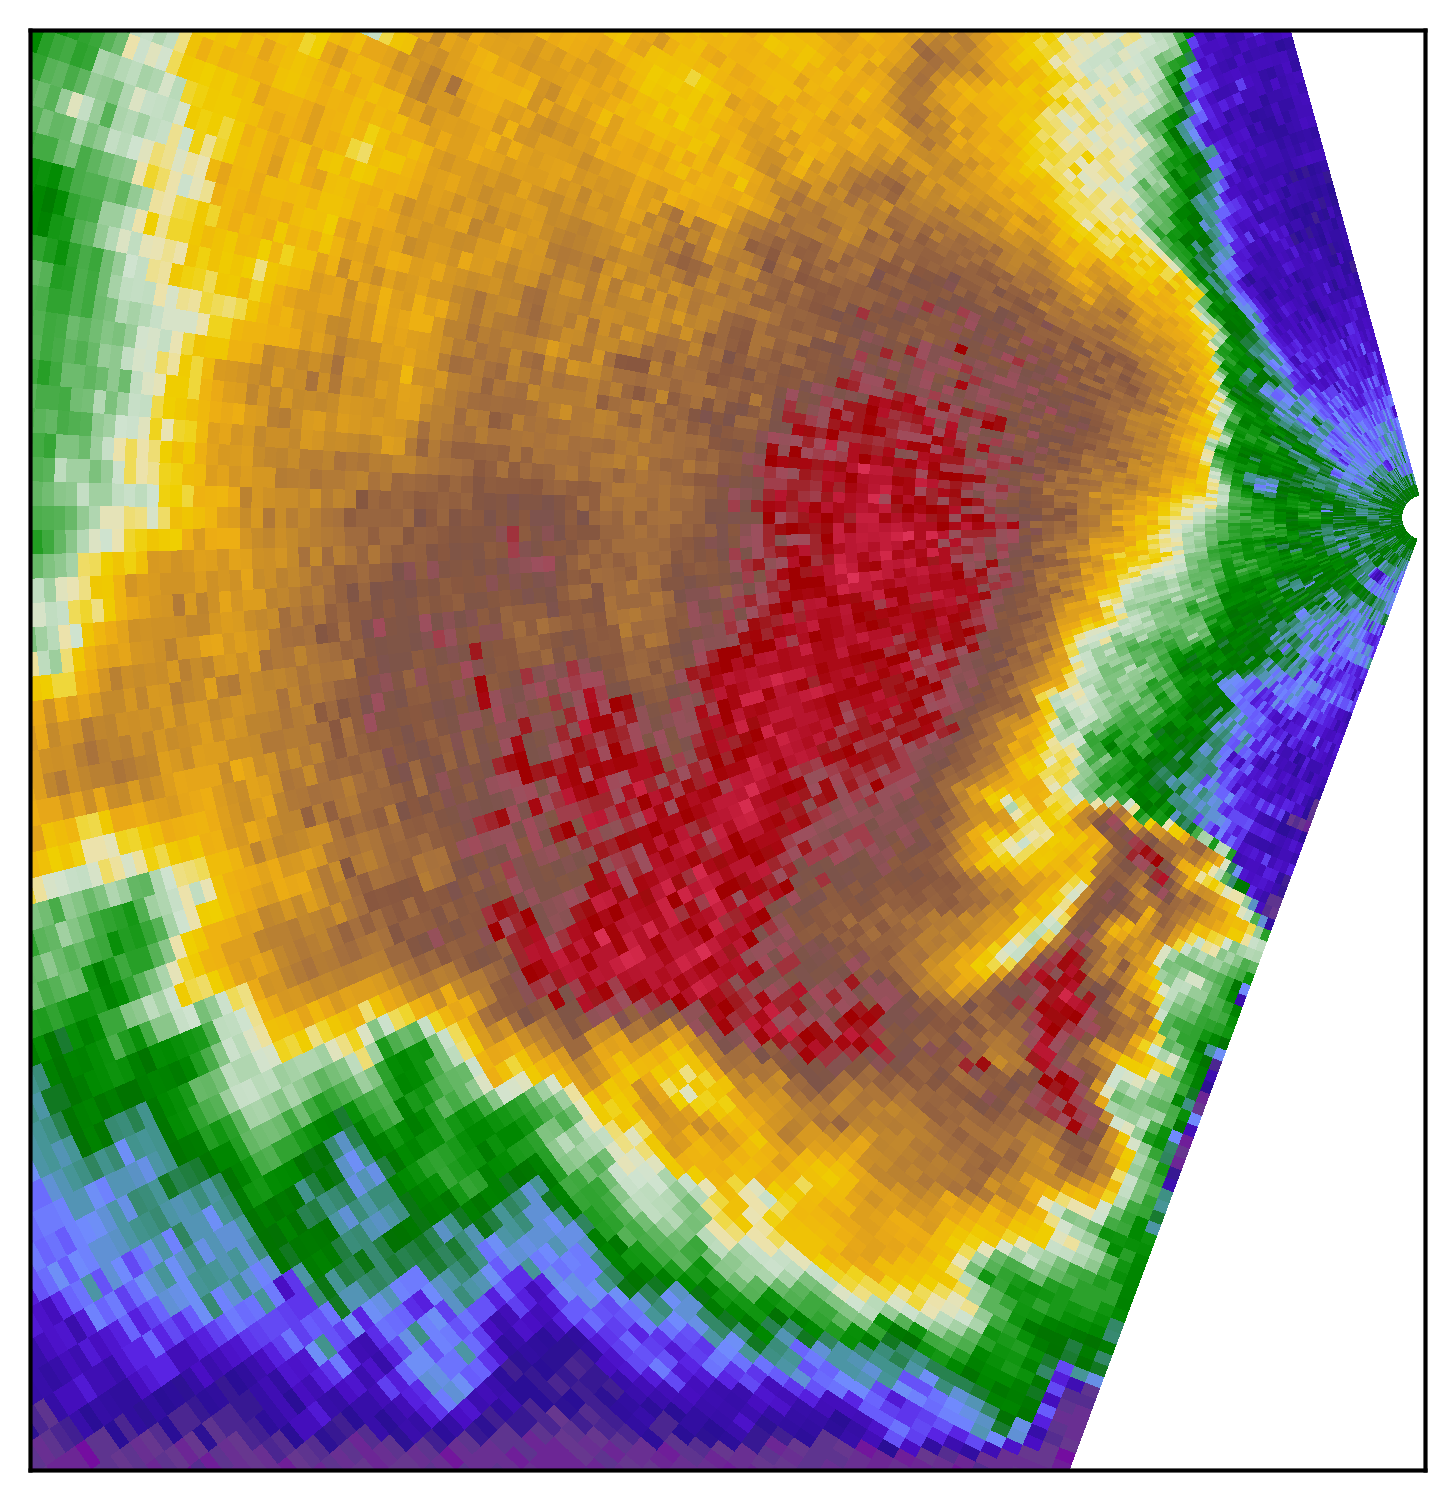
\includegraphics[scale=0.17]{figures/title_ppi.png}}

\begin{document}

\begin{frame}
	\titlepage
\end{frame}

\begin{frame}{Outline}
    \tableofcontents
\end{frame}

\section{Motivation}
\stepcounter{subsection}
\begin{frame}[<+->]
	\frametitle{Attenuating Systems}
	\begin{itemize}
		\item Proliferation of systems at attenuating wavelengths (C and X bands)
		\item Can be cheaper
		\item Better angular resolution
		\item Better sensitivity
	\end{itemize}
\end{frame}

\begin{frame}
	\frametitle{Applications}
	\begin{itemize}[<+->]
		\item Any quantitative use of the data necessitates correction for attenuation
		\item QPE
		\item Hydrometeor Classification
		\item 3dB error -> 64\% change in rain rate
	\end{itemize}
\end{frame}

\begin{frame}
	\frametitle{Attenuation Correction}
	\begin{itemize}[<+->]
		\item Many different algorithms in the literature
		\item Ones examined here:
		\begin{itemize}
			\item Linear $\Phi_{DP}$
			\item ZPHI
			\item Self-Consistent
		\end{itemize}
		\item Also testing modifications to self-consistent to improve robustness
		\item All of these rely upon empirically determined coefficients
		\item Which necessitates making certain assumptions (temperature,
		DSD, shape, etc.)
	\end{itemize}
\end{frame}

\begin{frame}[<+->]
	\frametitle{Testing Corrections}
	\begin{itemize}	
		\item Testing of these techniques usually rely upon comparison with
		unattenuated (S-band) data
		\item Another method involves examining reduction in QPE bias upon correction
		\item Instead here we use simulated data to provide data with and without
		attenuation
		\item Simulator allows changing assumptions to see impacts on correction
		\item Simulator also allows changing radar configuration
	\end{itemize}
\end{frame}

\section{Simulation}
\stepcounter{subsection}
\begin{frame}
  \frametitle{Simulator}
  \begin{itemize}[<+->]
  	\item Numerical cloud model output provides needed environmental information
  	\only<1>{\begin{itemize}
  		\item<1> Hydrometeor content
  		\item<1> Wind components
  		\item<1> Thermodynamic information
  		\end{itemize}}
  	\item Calculate scattering parameters from hydrometeor information and (optionally) temperature
  	\item Propagate discretized radar pulse through simulation grid
  	\item During propagation, accumulate phase shift and attenuation
  	\item Use scattering together with radar equation to synthesize radar signal
  	\item Includes antenna pattern (with optional sidelobes), range weighting, and noise
  \end{itemize}
\end{frame}

\begin{frame}[<+->]
	\frametitle{Signal Synthesis}
	\begin{itemize}
		\item Each pulse element gets assigned values from the source fields using 
		nearest neighbor sampling
		\item Complex signal values for each element are calculated as:
		\begin{align}
			A_{kh} &= \sqrt{P_{kh}} w_{1k} e^{-j\theta_k} \\
	A_{kv} &= \sqrt{P_{kv}} \left(\rho_{HVk} w_{1k} + \sqrt{1 - \rho_{HVk}^2} w_{2k} \right) e^{-j\theta_k} \\
    \theta_k &= \theta^n_k + \delta_k + \phi_k\\
    \theta^n_k &= \theta^{n-1}_k + \frac{4 \pi V_{rk} T_s}{\lambda}\\
    \theta^0_k &= 0
    \end{align}
		\item $w_{1k}$ and $w_{2k}$ are independent, random samples from a complex Gaussian distribution (Galati 1995)
		\item The $\theta_k$ tracks the phase at each element (the scattering center), which generates a phase shift with each pulse (Muschinski 1999)
	\end{itemize}
\end{frame}

\begin{frame}[<+->]
	\frametitle{Signal Synthesis (cont.)}
		\begin{itemize}
		\item Power at each element is calculated from radar equation:
		\begin{align}
		    P_k = \frac{P_t g^2 \lambda^2 f^4(\theta_k,\phi_k) |W(r_0, r)|^2 \eta_k}
		        {(4 \pi)^3 l_k^2(r) r^2}
		\end{align}
		\item Correlation between polarizations uses theoretical $\rho_{HV}$ from scattering calculation (Galati 1995)
		\item Each polarization is attenuated and phase-shifted separately on a per-element basis
		\item Radar IQ sample is generated by integrating the complex signal
		values across all elements and adding to a single white noise value
	\end{itemize}
\end{frame}

\begin{frame}
	\frametitle{Single-Polarization Moment Estimation}
	\begin{align}
	    \hat{R}(l) &= \sum_{n=0}^{N-l-1} V(n + l) V^*(n) \\
	    \hat{P} &= \hat{R}(0) \\
	    \hat{V_r} &= \frac{-\lambda}{4 \pi \,T_s} \arg{\hat{R}(1)} \\
	    \hat{\sigma}_v &= \frac{\lambda}{2 \pi \,T_s \sqrt{2}}
	        \left[\ln{\left|\frac{\hat{R}(0)}{\hat{R}(1)}\right|}\right]^{\frac{1}{2}}
	\end{align}
\end{frame}

\begin{frame}
	\frametitle {Dual-Polarization Moment Estimation}
	\begin{align}
	    \hat{R}_{v,h}(l) &= \sum_{n=0}^{N-l-1} V_{v}(n+l) V_{h}^*(n) \\
	    \hat{Z}_{DR} & = \frac{\hat{P}_h - \hat{N}_h}{\hat{P}_v - \hat{N}_v} \\
	    |\hat{\rho}_{co}| &= \frac{|\hat{R}_{v,h}(0)|}{\sqrt{\hat{P}_h\hat{P}_v}} \\
	    \hat{\phi}_{DP} &= \arg{\hat{R}_{v,h}(0)}
	\end{align}
\end{frame}

\begin{frame}
	\frametitle{Scattering}
	\begin{itemize}
		\item Configurable scattering models
		\begin{itemize}
			\item T-Matrix
			\item Rayleigh-Gans
			\item Mie
			\item Rayleigh
			\end{itemize}
		\item Configurable drop shape model
		\begin{itemize}
			\item Brandes et al. (2004) polynomial model
			\item Pruppacher and Beard (1970) linear model
			\end{itemize}
		\item Wavelength- and temperature-dependent complex dielectric constant (Ray 1972, Liebe 1991)
		\item Width of canting angle distribution can also be controlled
	\end{itemize}
\end{frame}

\begin{frame}[<+->]
	\frametitle{Microphysics}
	\begin{itemize}
		\item Native model microphysics scheme is two-moment (Ziegler 1985)
		\item Model distribution is a gamma distribution for volume of drops
		\item However this distribution is not well-suited to radar
		\begin{align}
			N(V) = \frac{N (\nu + 1)^{\nu + 1}}{V_0 \Gamma(\nu + 1)}
        \left(\frac{V}{V_0}\right)^{\nu}
        \exp\left[{-(\nu + 1) \frac{V}{V_0}}\right]
		\end{align}
	\end{itemize}
\end{frame}

\begin{frame}
	\frametitle{Microphysics (cont.)}
	\begin{center}
		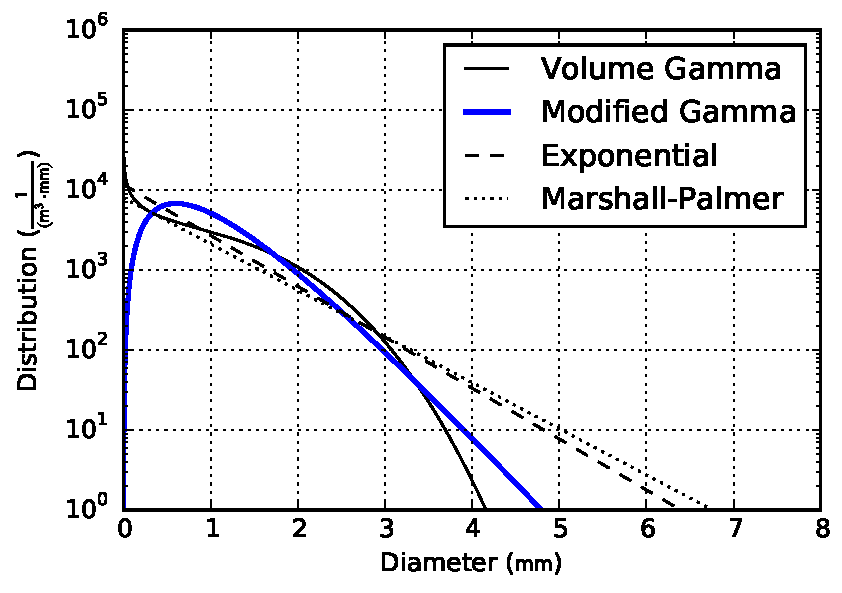
\includegraphics[scale=0.6]{figures/distribution-comparison.pdf}
	\end{center}
\end{frame}

\begin{frame}[<+->]
	\frametitle{Microphysics (cont.)}
	\begin{itemize}
		\item Much better to use modified gamma distribution (Ulbrich 1983)
		\item Three parameter distribution
		\begin{align}
			N(D) = N_0 D^\mu e^{(-\Lambda D)}
		\end{align}
		\item Only two moments $N_0 (<D^0>)$ and $q_r (<D^3>)$
	\end{itemize}
\end{frame}

\begin{frame}[<+->]
	\frametitle{Microphysics (cont.)}
	\begin{itemize}
		\item Attempted to use $\mu-\Lambda$ relation of Zhang et al. (2001)
		\begin{align}
			\mu = \num{-0.016} \Lambda^2 + \num{1.213} \Lambda - \num{1.957}
		\end{align}
		\item This yields a sixth order polynomial in $\Lambda$
		\item Though it generally has two real, positive roots
		\item Options for choosing root tested: min, max, closest to chosen $\Lambda$, closest to chosen $\mu$
	\end{itemize}
\end{frame}

\begin{frame}[<+->]
	\frametitle{Microphysics (cont.)}
	\begin{itemize}
		\item Instead, we add a constraint to conserve the (approximate) radar reflectivity factor of the model ($<D^6> = \left(\frac{6}{\pi}\right)^2<V^2>$)
		\item By combining the 0th, 3rd, and 6th moments of D we get:
		\begin{align}
			\frac{\overline{D^3}^2}{\overline{D^0}\,\overline{D^6}} =  \frac{\nu + 1}{\nu + 2}
		\end{align}
		\item This yields the following polynomial
		\begin{align}
			\frac{\num{5}}{\num{6}} \mu^3 + \frac{\num{7}}{\num{2}} \mu^2 - \frac{\num{4}}{\num{3}} \mu - \num{14} = 0
		\end{align}
		\item Which has a positive root of $\mu=\num{1.81}$
	\end{itemize}
\end{frame}

\begin{frame}
	\frametitle{Microphysics (cont.)}
	\begin{center}
		\includegraphics[scale=0.6]{figures/atten-distribution.pdf}
	\end{center}
\end{frame}

\begin{frame}
	\frametitle{Canting Distribution}
	\begin{itemize}
		\item Utilizes axial distribution for distribution of particle canting angles (Mardia 1972)
		\item Describes the distribution of a two-dimensional orientation angle in which one of the components is fixed at \SI{90}{\degree}
		\item Given by:
		\begin{align*}
			g_A(\theta) &= b(\kappa) \exp(-\kappa \cos^2{\theta}) \sin{\theta} \\
			b(\kappa) &= \frac{1}{2 \int_0^1 \exp(-\kappa t^2)\,dt}
		\end{align*}
	\end{itemize}
\end{frame}

\begin{frame}
	\frametitle{Canting Distribution (cont.)}
	\begin{center}
		\includegraphics[scale=0.5]{figures/angular-distribution.pdf}
	\end{center}	
\end{frame}

\section{Example Output}
\stepcounter{subsection}
\begin{frame}
	\frametitle{Model Field}
	\begin{center}
		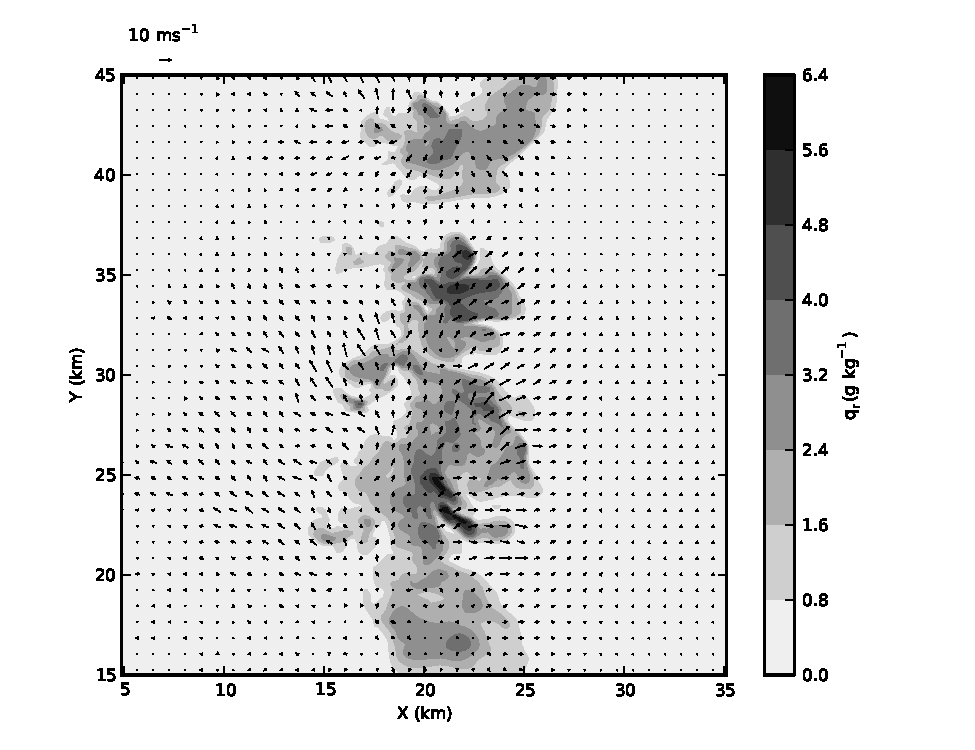
\includegraphics[scale=0.5]{figures/commas_wz_3600_qr_wind_vectors.pdf}	
	\end{center}
\end{frame}

\begin{frame}
	\frametitle{Example Configuration}
	\begin{center}
	    \begin{tabular}{ | l | l | }
	        \hline
	        Antenna gain & \SI{45.5}{dB} \\
	        Peak power & \SI{250}{\kilo\watt} \\
	        First range gate & \SI{500}{\meter} \\
	        Noise power & \SI{-113}{dBm} \\
	        Elevation & \SI{0.5}{\degree} \\
	        PRT & \SI{0.667}{\milli\second} \\
	        Rotation Rate & \SI{20}{\degree\per\second} \\
	        Pulses per radial & \num{75} \\
	        Gate length & \SI{125}{\meter} \\
	        Antenna Limits & Main-lobe only \\
			Wavelength &  \SI{5.5}{\centi\meter} \\
			Beamwidth & \SI{1.0}{\degree} \\
			Radial Spacing & \SI{1.0}{\degree} \\
			\hline
	    \end{tabular}
	\end{center}
\end{frame}

\begin{frame}
	\frametitle{Example Images}
	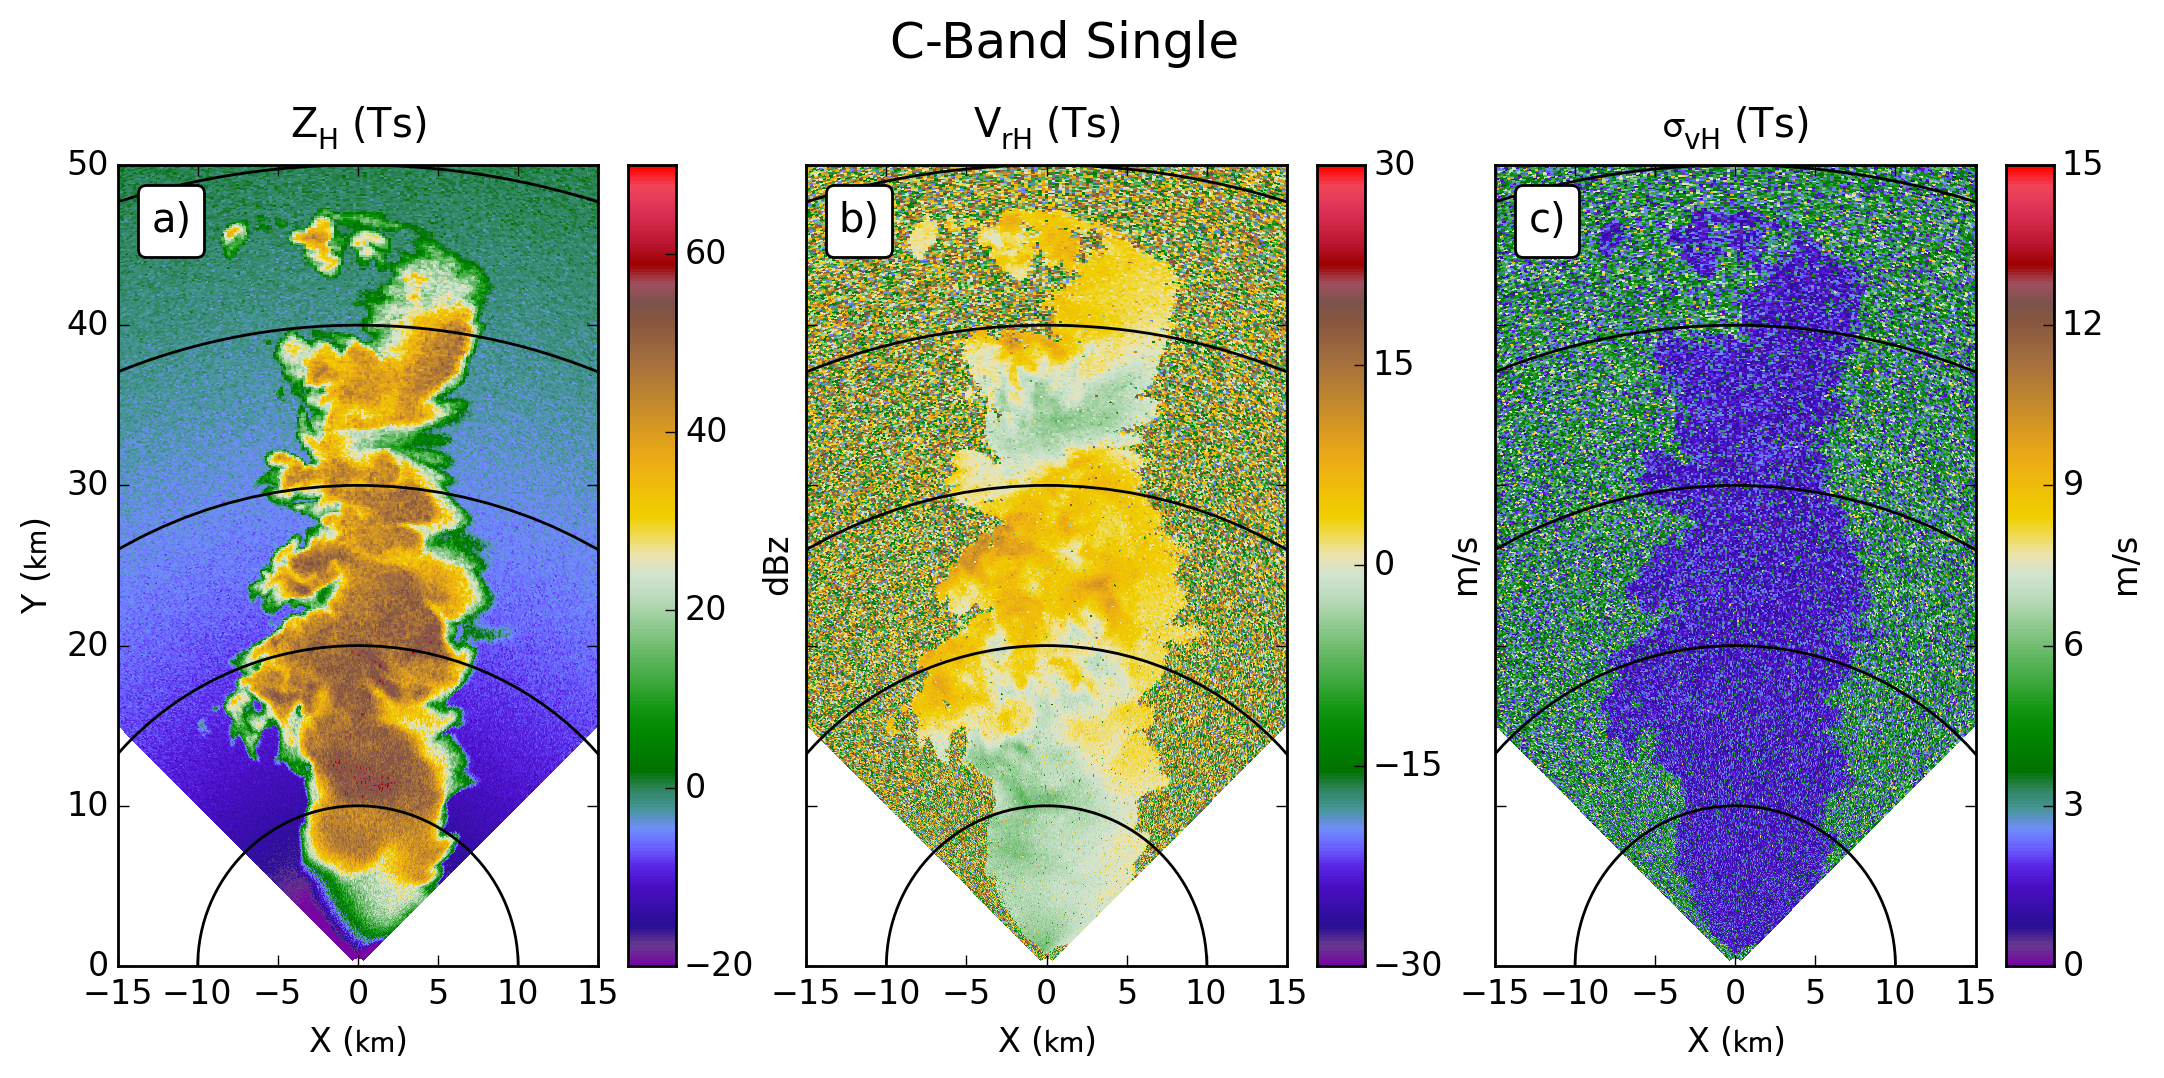
\includegraphics[scale=0.4]{figures/C_Single.png}
\end{frame}

\begin{frame}
	\frametitle{Example Images (cont.)}
	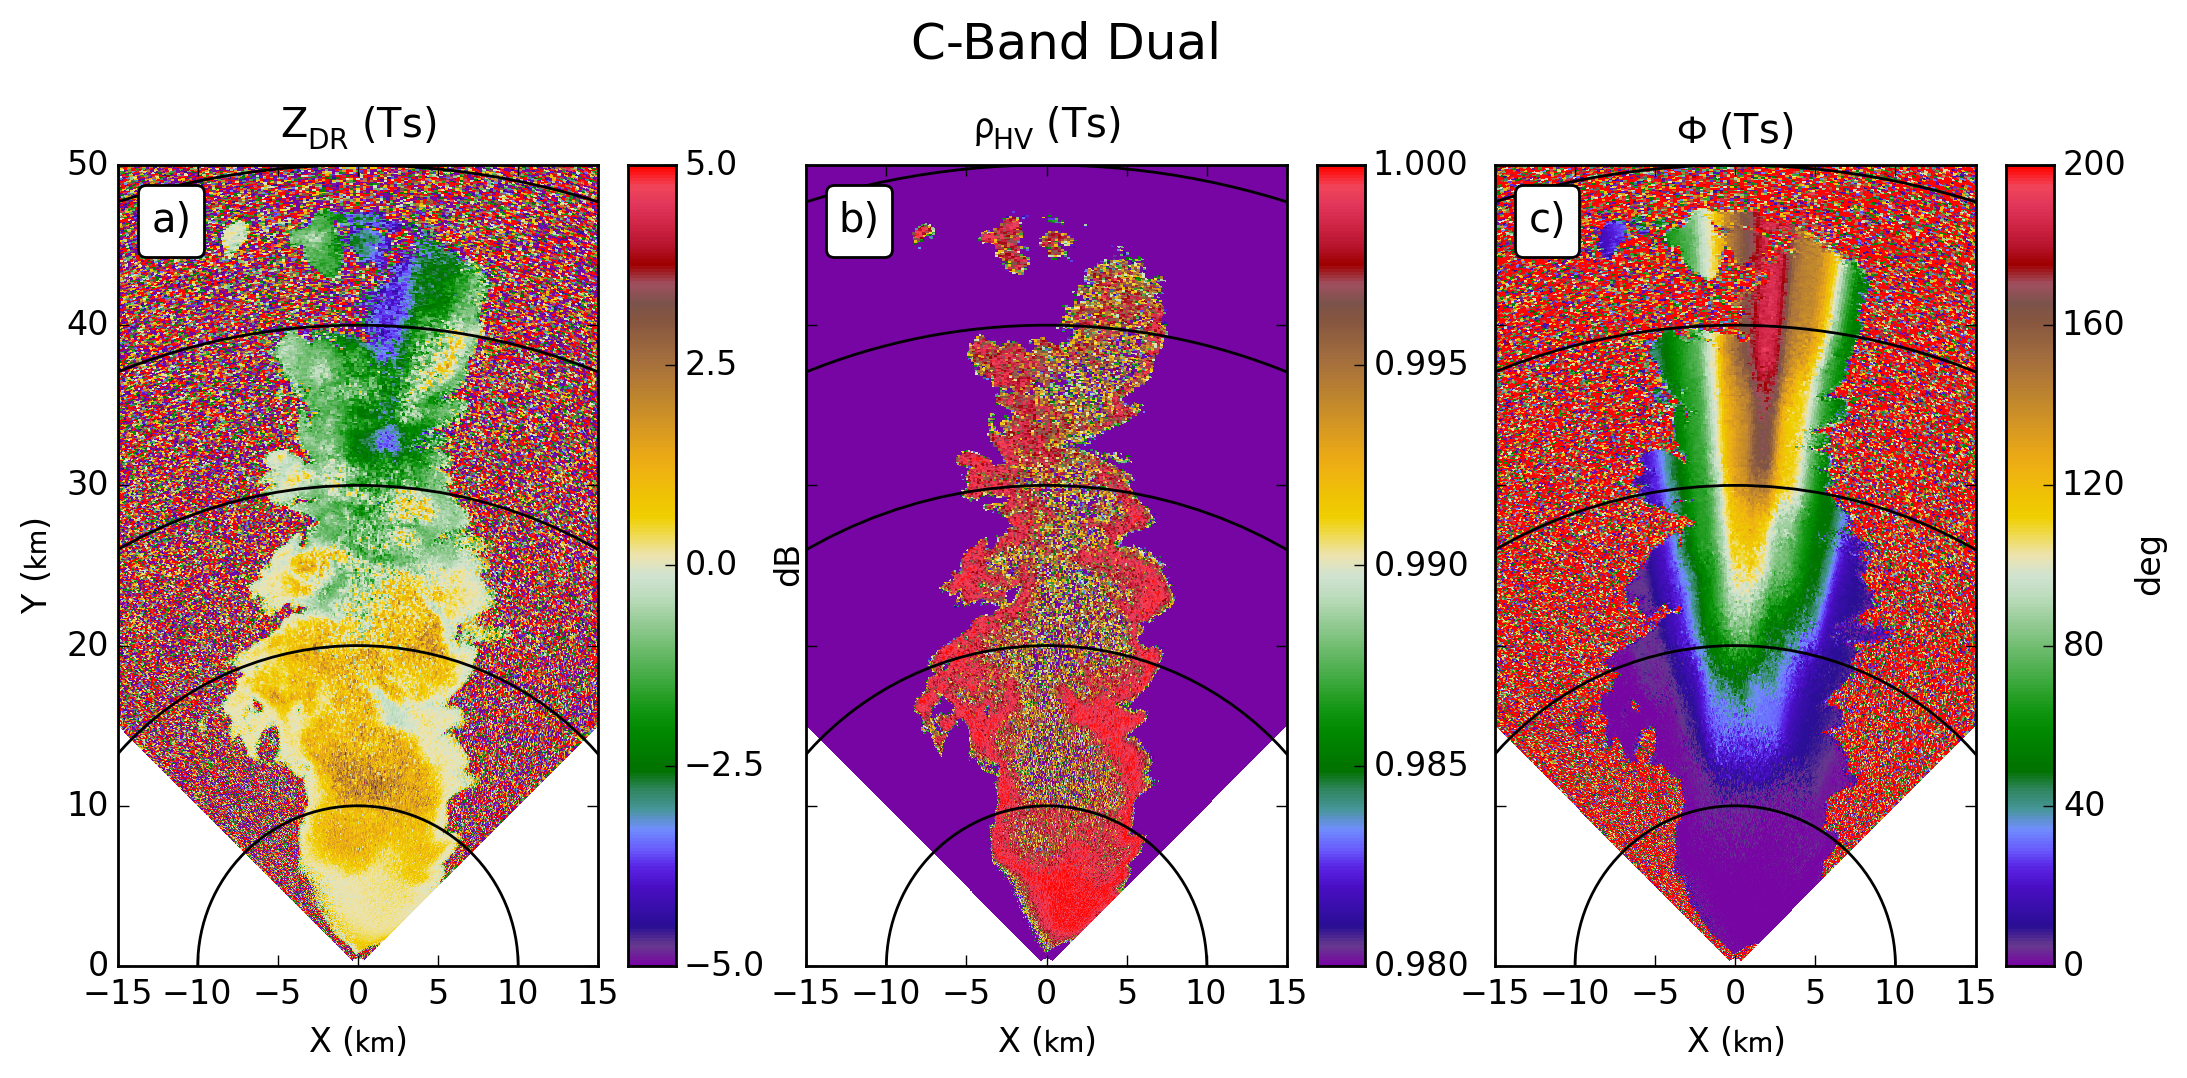
\includegraphics[scale=0.4]{figures/C_Dual.png}
\end{frame}

\begin{frame}
	\frametitle{Example Images (cont.)}
	\begin{center}
		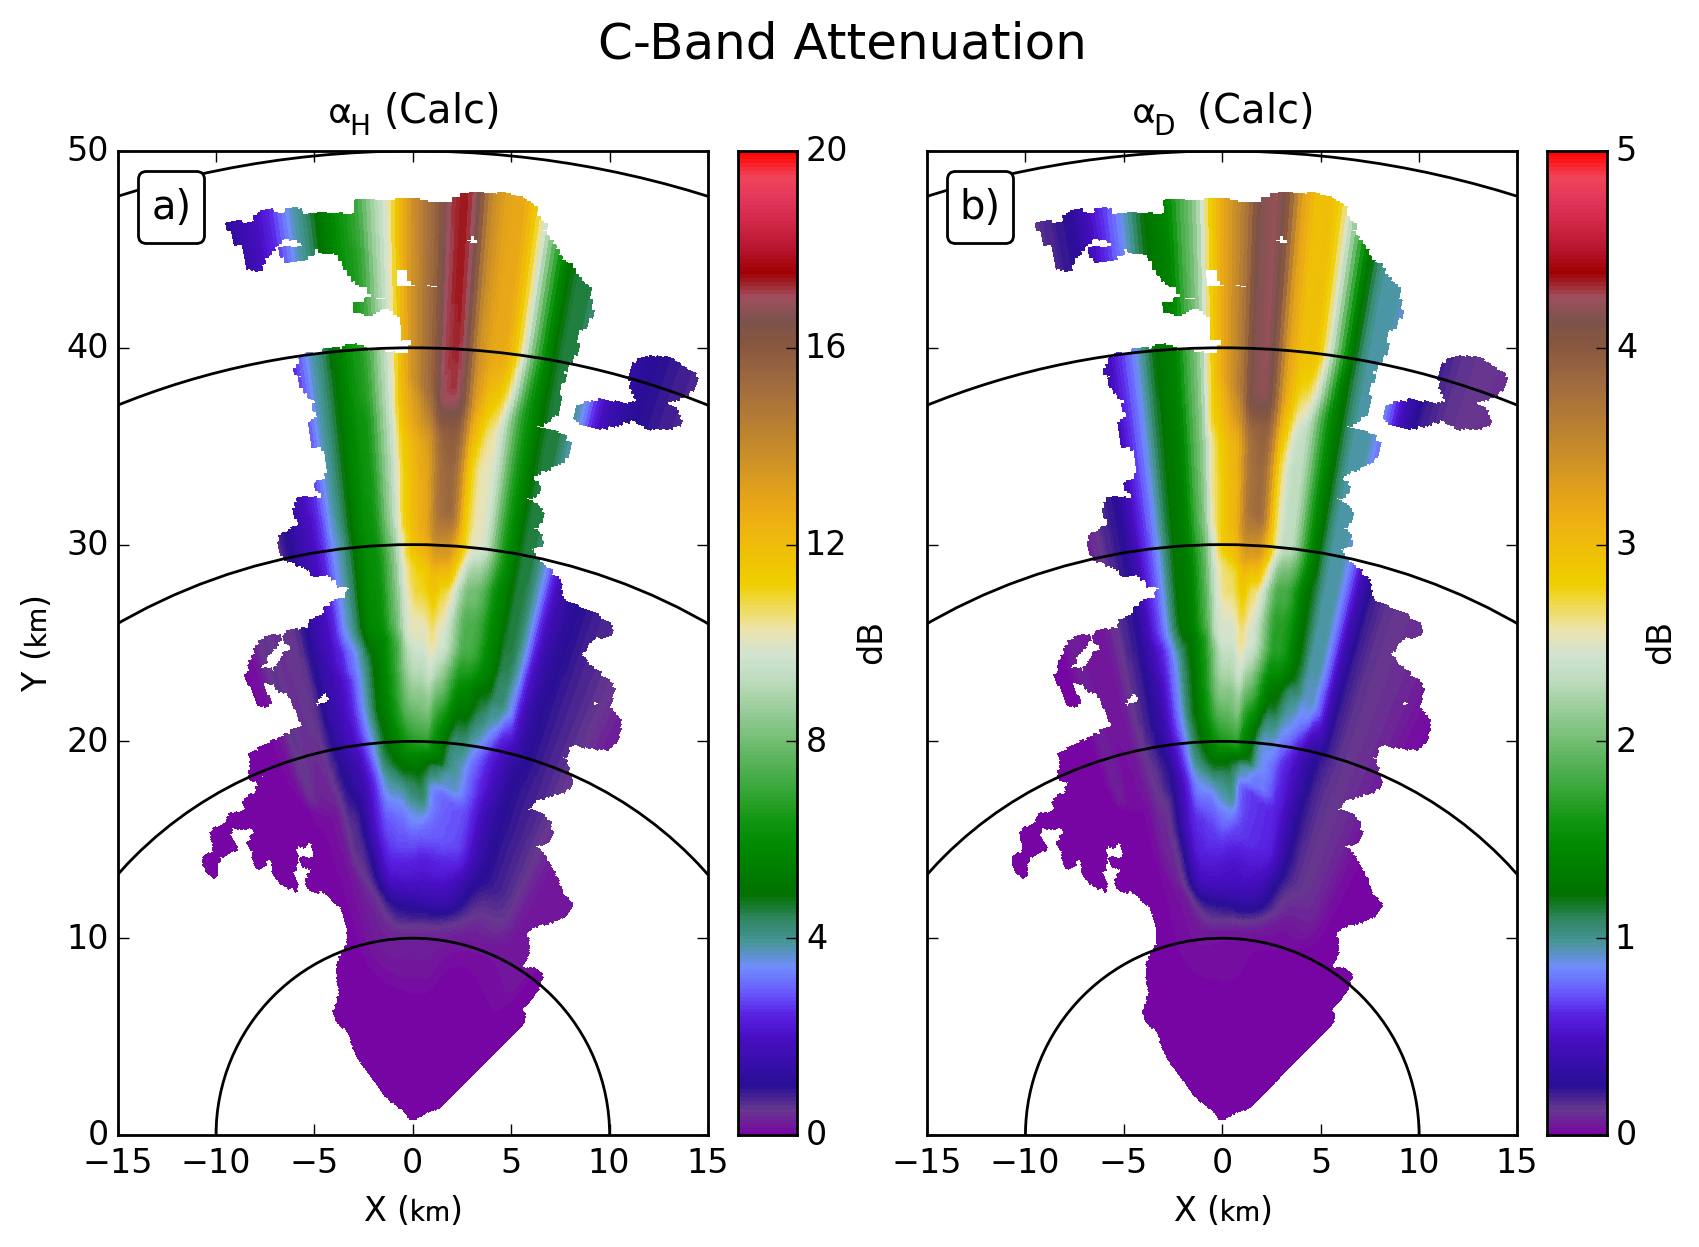
\includegraphics[scale=0.4]{figures/C_Attenuation.png}
	\end{center}
\end{frame}

\begin{frame}
	\frametitle{Example Images (cont.)}
	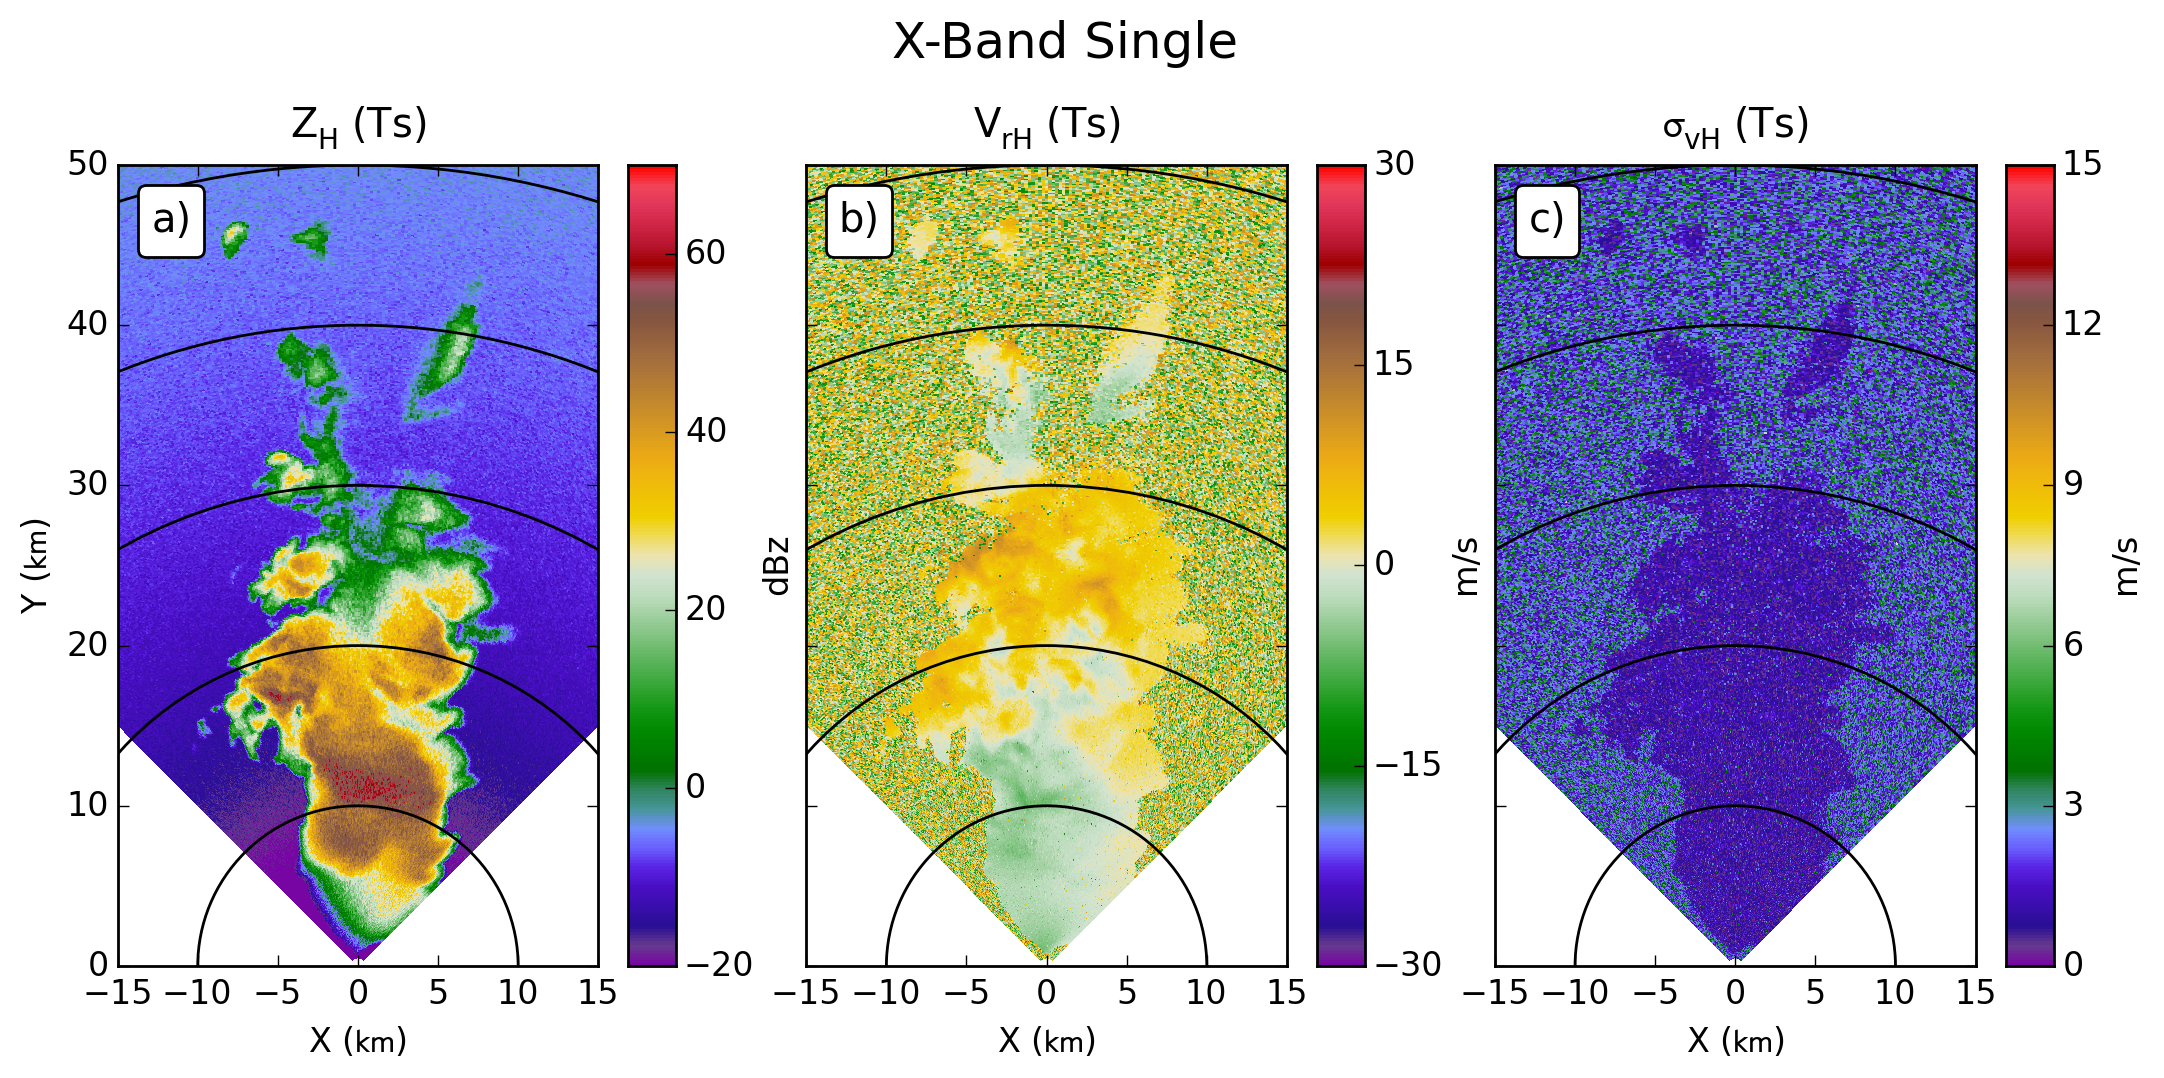
\includegraphics[scale=0.4]{figures/X_Single.png}
\end{frame}

\begin{frame}
	\frametitle{Example Images (cont.)}
	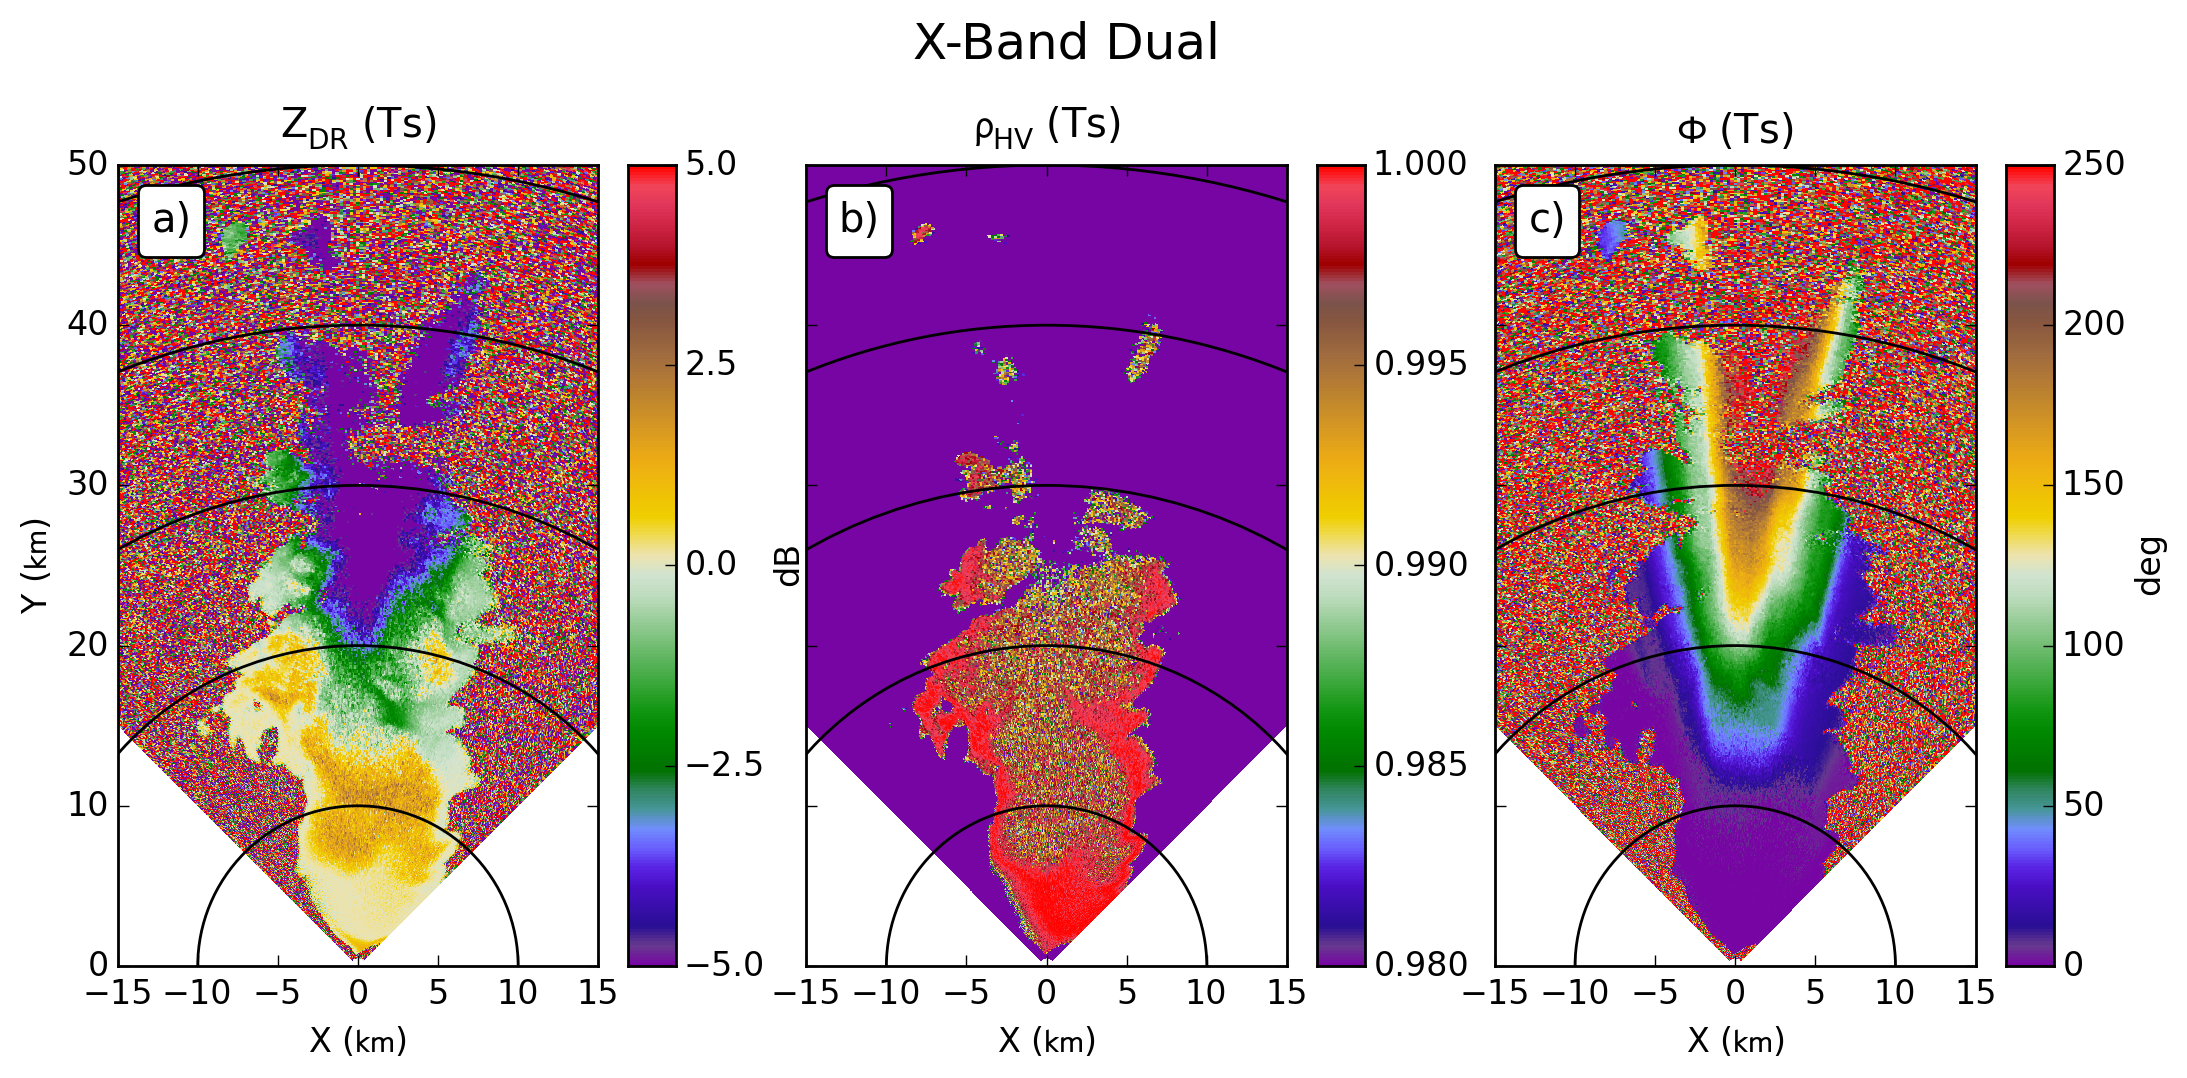
\includegraphics[scale=0.4]{figures/X_Dual.png}
\end{frame}

\begin{frame}
	\frametitle{Example Images (cont.)}
	\begin{center}
		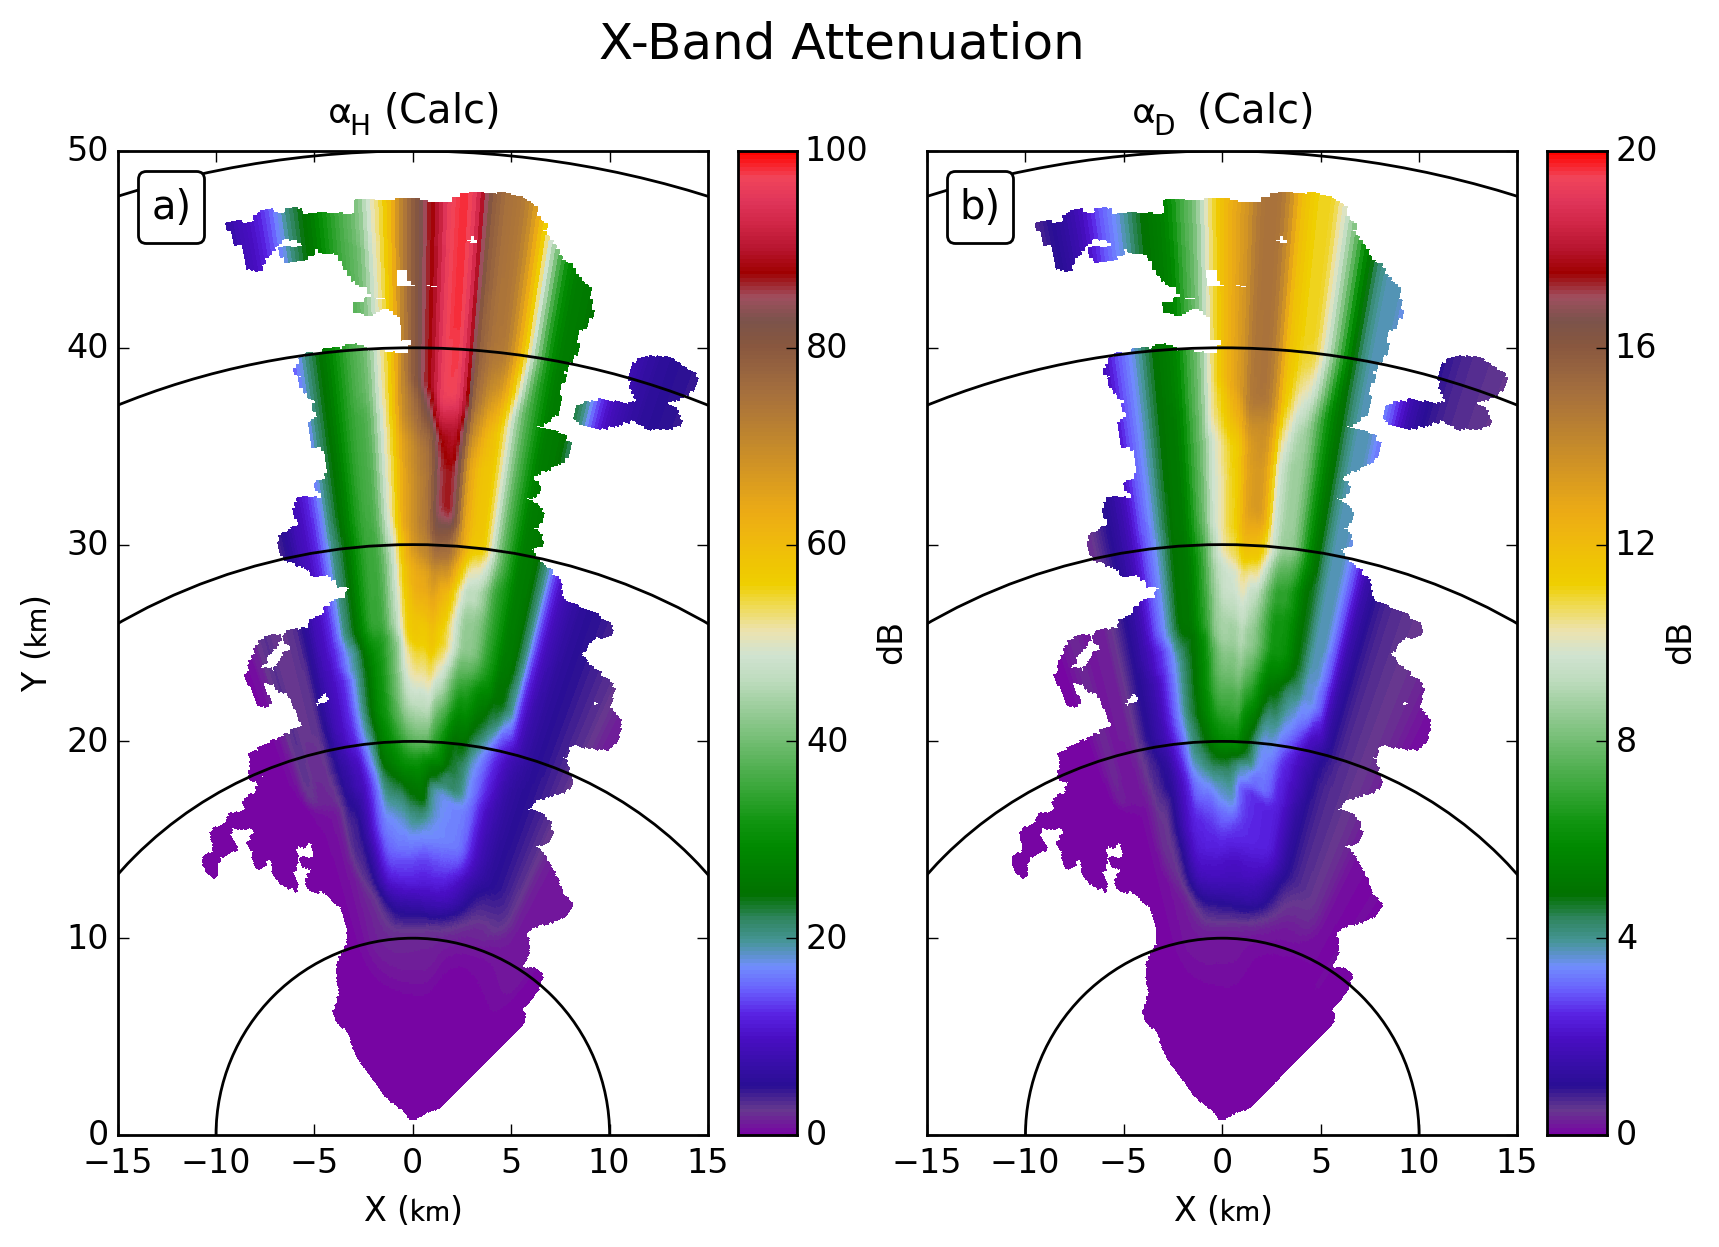
\includegraphics[scale=0.4]{figures/X_Attenuation.png}
	\end{center}
\end{frame}

\section{Algorithms}
\stepcounter{subsection}
\begin{frame}
	\frametitle{Linear $\Phi_{DP}$}
	\begin{itemize}
		\item Described by Bringi et al. (1990)
		\item Formulate linear relationship between $K_{DP}$ and $A_H$
		\begin{align*}
			A_H &= \beta_H K_{DP} \\
			A_D &= \beta_D K_{DP}
		\end{align*}
		\item Leads to direct conversion between $\Phi_{DP}$  and  both
				$\alpha_H$ and $\alpha_D$
	\end{itemize}
\end{frame}

\begin{frame}
	\frametitle{ZPHI}
	\begin{itemize}
		\item Described by Testud et al. (2000)
		\item Based around Hitschfeld (1954) reflectivity-based method
		\item Uses linear $\Phi_{DP}$ to provide constraint
			\begin{align*}
			I(r, r_0) &= \num{0.46}b\int_r^{r_0}Z_a^b(s)\,ds \\
			\alpha(r_0) &= \frac{Z_a^b(r_0)}{I(r_1,r_0)} \lbrace 10^{\num{0.1}b\gamma\Delta\Phi} - 1\rbrace \\
			\alpha(r) &= \frac{Z_a^b(r)}{I(r_1,r_0) + \lbrace 10^{\num{0.1}b\gamma\Delta\Phi} - 1\rbrace I(r, r_0)}
			  \times \lbrace 10^{\num{0.1}b\gamma\Delta\Phi} - 1\rbrace
			\end{align*}
	\end{itemize}
\end{frame}

\begin{frame}
	\frametitle{Self-Consistent}
	\begin{itemize}
		\item Described by Bringi et al. (2001)
		\item Adds a "self-consistent" restriction to ZPHI
		\item Attempts to automatically find the optimal value of $\gamma$
		on a ray by ray basis
			 \begin{align*}
			\phi_{DP}^c(r;\gamma) &= 2 \int_{r_0}^r \frac{A_h(s;\gamma)}{\gamma}\,ds \\
			\gamma_{min} &\leq \gamma \leq \gamma_{max} \\
			Error &= \sum_{j=1}^N \left| \Phi_{DP}^{filt}(r_j) - \Phi_{DP}^c(r_j;\gamma) \right|
			\end{align*}
	\end{itemize}
\end{frame}

\begin{frame}[<+->]
	\frametitle{Modified Self-Consistent}
	\begin{itemize}
		\item In the process of doing this study, noticed that the errors in ZPHI
		had an oscillatory behavior
		\item Also noticed some bad rays when there was less data coverage
		\item To address this, a modified version of Self-Consistent algorithm
		was also tested
		\item This version, after finding the optimal $\gamma$ for each ray
		takes the median value of all $\gamma$ values and uses it for all rays
		\item Attempts to smooth out variations in $\gamma$, trading a bit of
		optimization for robustness
	\end{itemize}
\end{frame}

\begin{frame}[<+->]
	\frametitle{Coefficient Regression}
	\begin{itemize}
		\item Need to determine own set of coefficients for algorithms
		\item All relations some kind of power law
		\item Original algorithms all use different assumptions
		\item Make best-case coefficients using actual data from model and
		the assumptions used in simulation
		\item Brandes et al. (2004) shape model at \SI{283}{\kelvin} with a canting distribution width of 10
	\end{itemize}
\end{frame}

\begin{frame}
	\frametitle{Coefficient Regression (cont.)}
	\begin{center}
		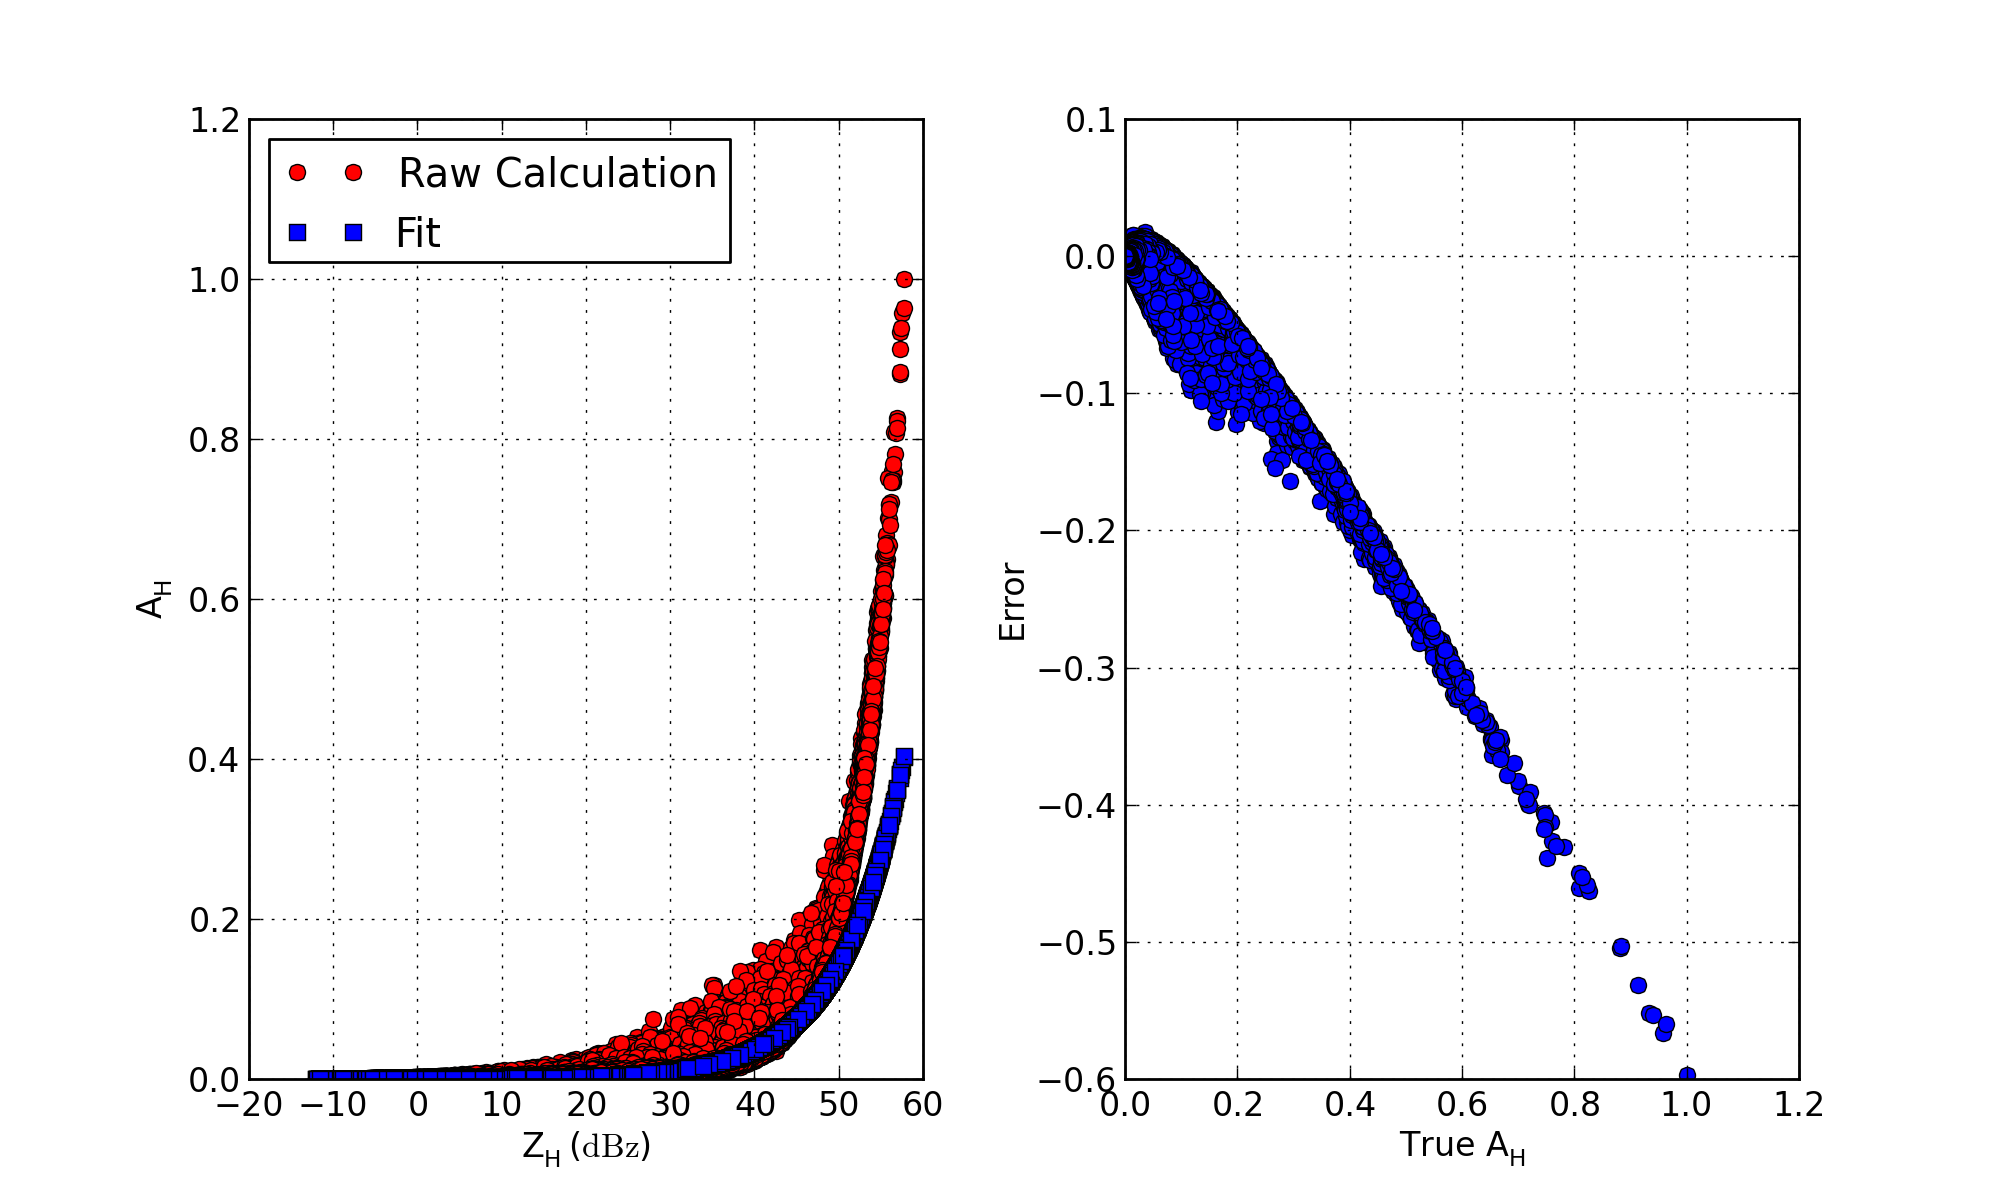
\includegraphics[scale=0.35]{figures/basic_power_law.png}
	\end{center}
	\begin{itemize}
		\item Clearly bias in the fit curve
	\end{itemize}
\end{frame}

\begin{frame}
	\frametitle{Coefficient Regression (cont.)}
	\begin{center}
		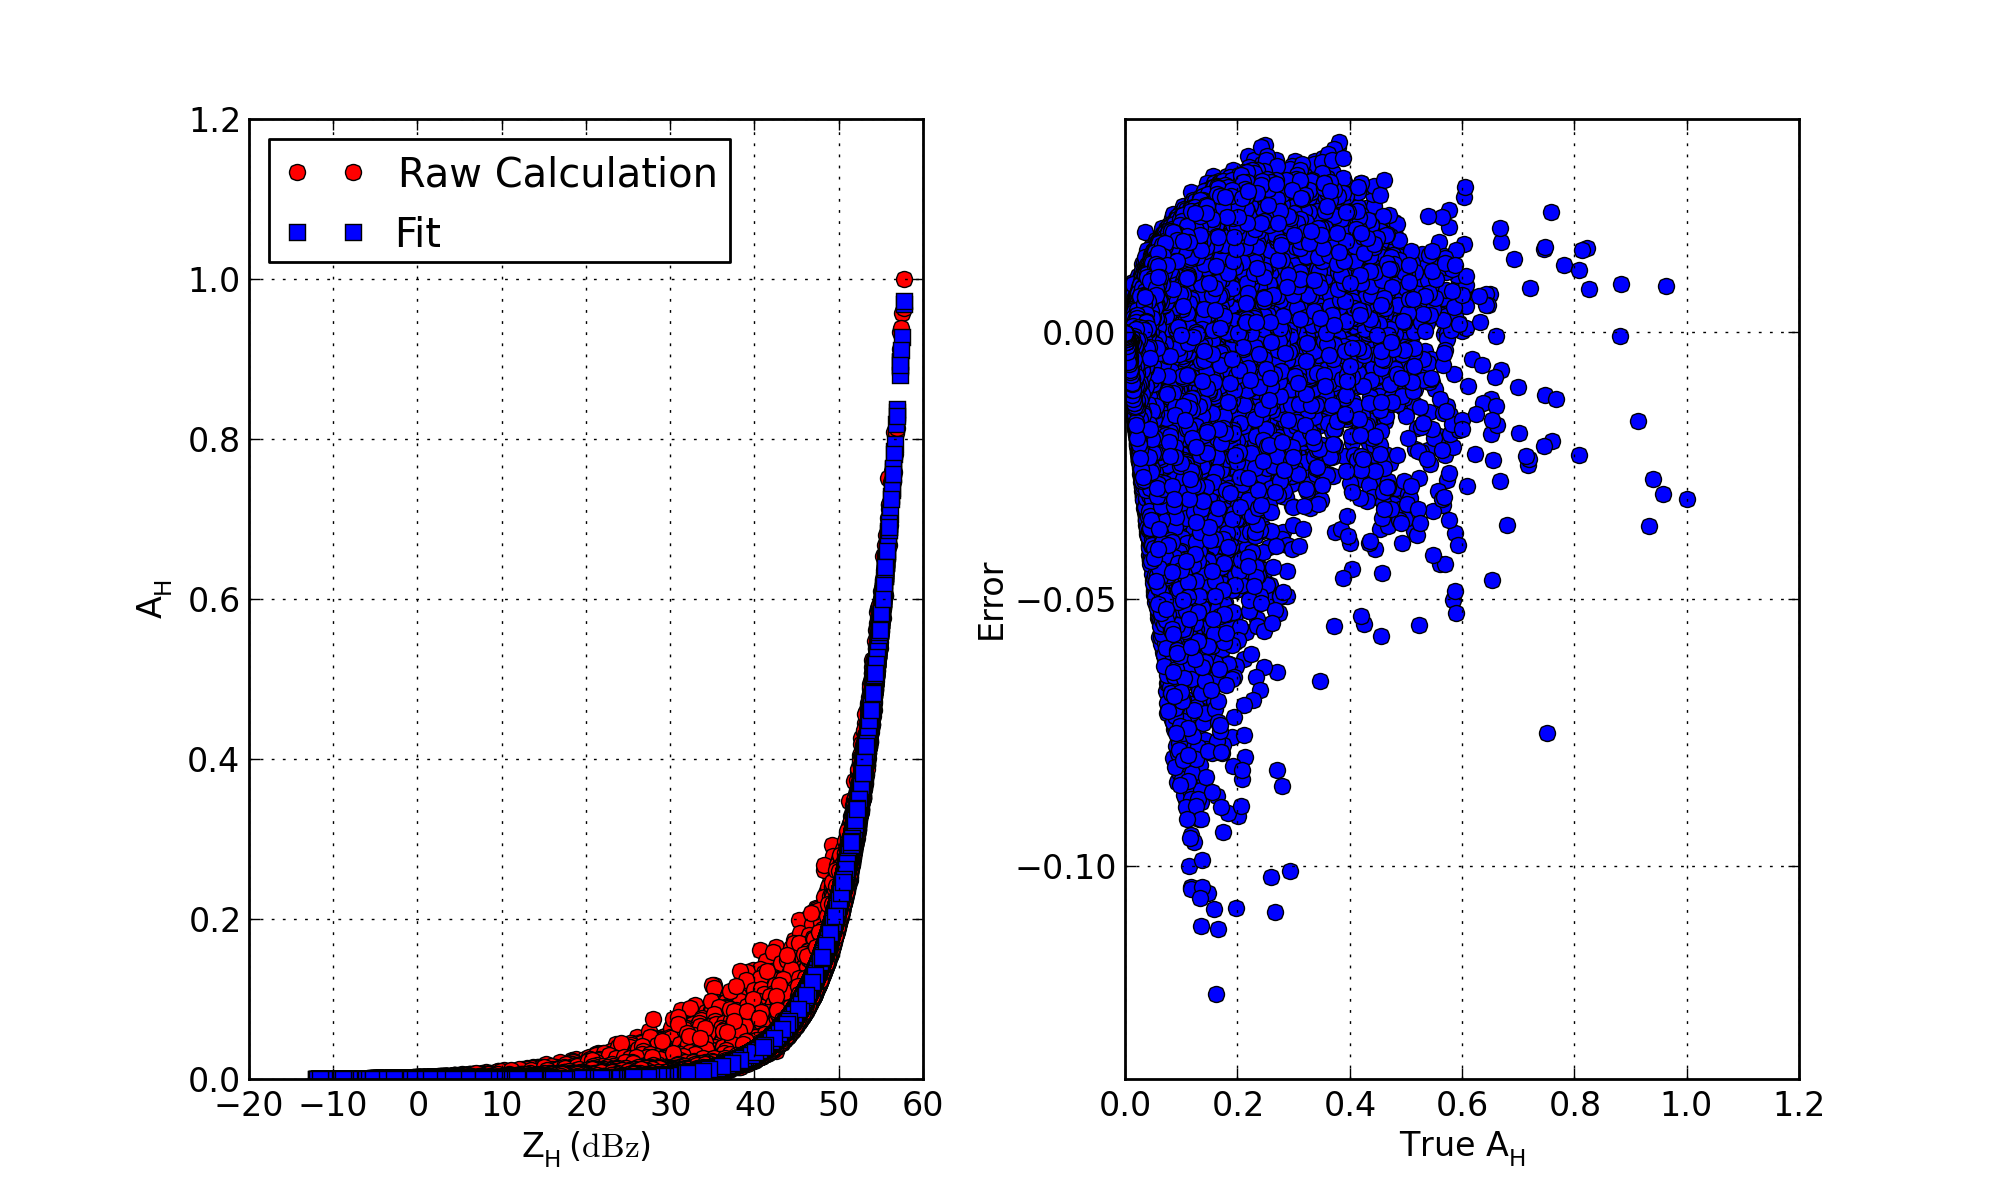
\includegraphics[scale=0.35]{figures/weighted_power_law.png}
	\end{center}
	\begin{itemize}
		\item Much better when using $A_H^2$ as the weights in regression
	\end{itemize}
\end{frame}

\begin{frame}
	\frametitle{Best-fit Coefficients}
    \begin{center}
	    \begin{tabular}{ | l | l | l |}
	        \hline
	        & \textbf{C-band} & \textbf{X-band}\\
	        \hline\hline
	        $\beta_H$ &  \num{0.7706} & \num{0.6214} \\
	        $\beta_V$ &  \num{0.8121} & \num{0.6813} \\
	        $\gamma_H$ & \num{0.1001} & \num{0.3316} \\
	        $\gamma_V$ & \num{0.0734} & \num{0.2789} \\
	        \hline
	    \end{tabular}
	\end{center}
\end{frame}

\section{Errors}
\stepcounter{subsection}
\subsection{Model Errors}
\begin{frame}
	\frametitle{Experimental Configuration}
	\begin{center}
	    \begin{tabular}{ | l | l | }
	        \hline
	        Antenna gain & \SI{45.5}{dB} \\
	        Peak power & \SI{250}{\kilo\watt} \\
	        First range gate & \SI{500}{\meter} \\
	        Noise power & \SI{-113}{dBm} \\
	        Elevation & \SI{0.5}{\degree} \\
	        PRT & \SI{0.667}{\milli\second} \\
	        Rotation Rate & \SI{20}{\degree\per\second} \\
	        Pulses per radial & \num{75} \\
	        Gate length & \SI{100}{\meter} \\
	        Antenna Limits & Main-lobe only \\
			Beamwidth & \SI{0.25}{\degree} \\
			Radial Spacing & \SI{0.25}{\degree} \\
			Scattering Model & T-Matrix \\
			\hline
	    \end{tabular}
	\end{center}
\end{frame}

\subsubsection{Control}
\begin{frame}
	\frametitle{Control: Matched Assumptions}
	\begin{center}
	    \begin{tabular}{ | l | l | }
	        \hline
	        Temperature & \SI{283}{\kelvin} \\
	        Drop Shape Model & Brandes \\
	        Wavelength & \SI{5.5}{\centi\meter}, \SI{3.21}{\centi\meter} \\
			\hline
	    \end{tabular}
	\end{center}	
\end{frame}

\begin{frame}
    \begin{center}
        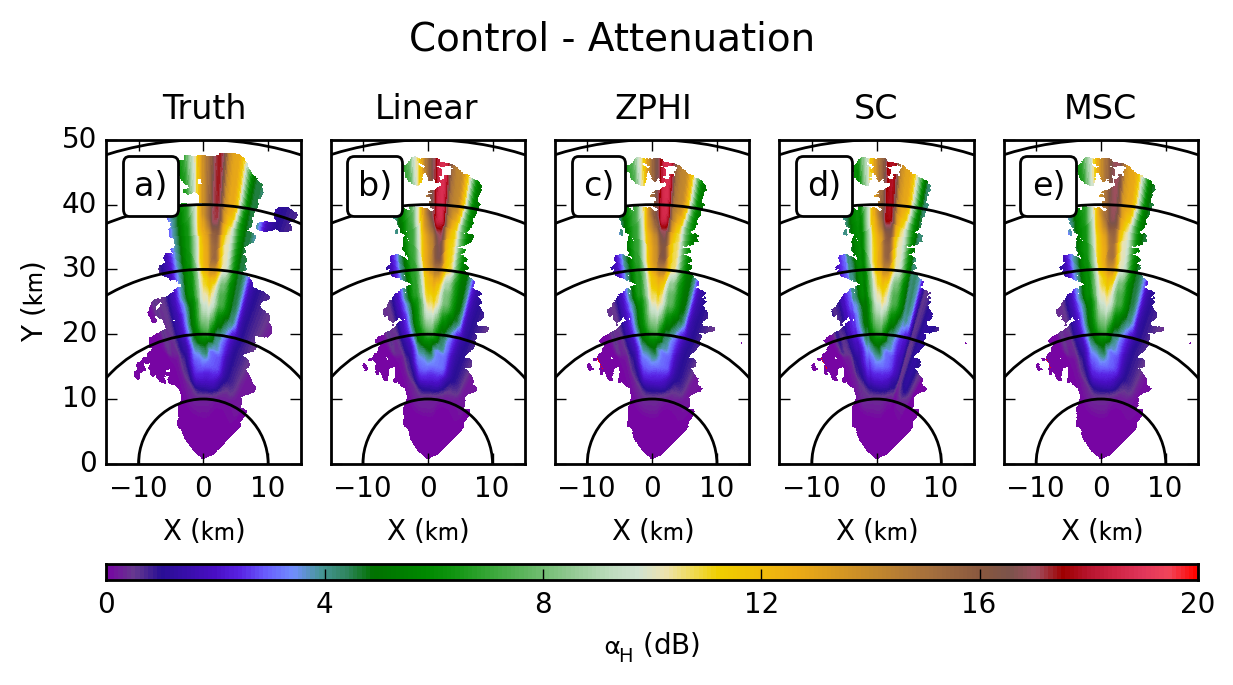
\includegraphics[scale=0.7]{figures/C_Control_Attenuation_H}
    \end{center}
\end{frame}

\begin{frame}
    \begin{center}
        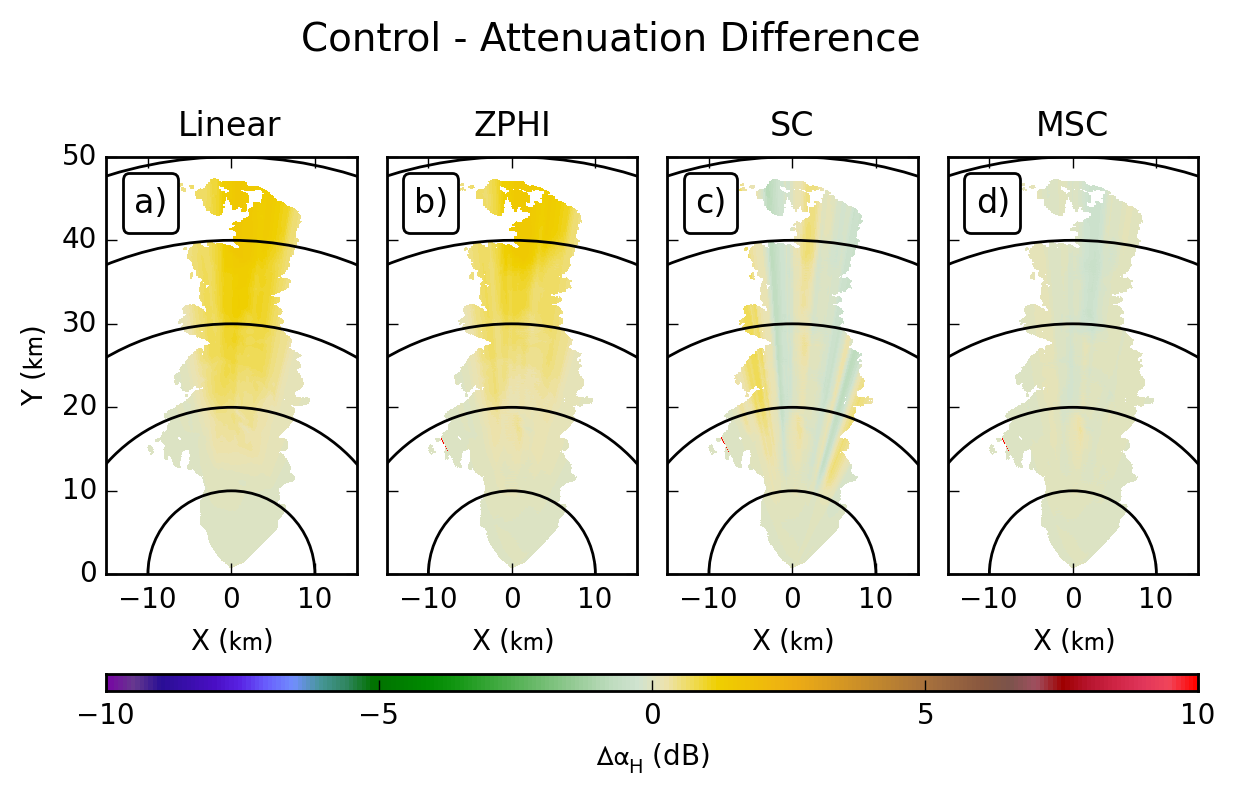
\includegraphics[scale=0.7]{figures/C_Control_Attenuation_Difference_H}
    \end{center}
\end{frame}

\begin{frame}
    \begin{center}
        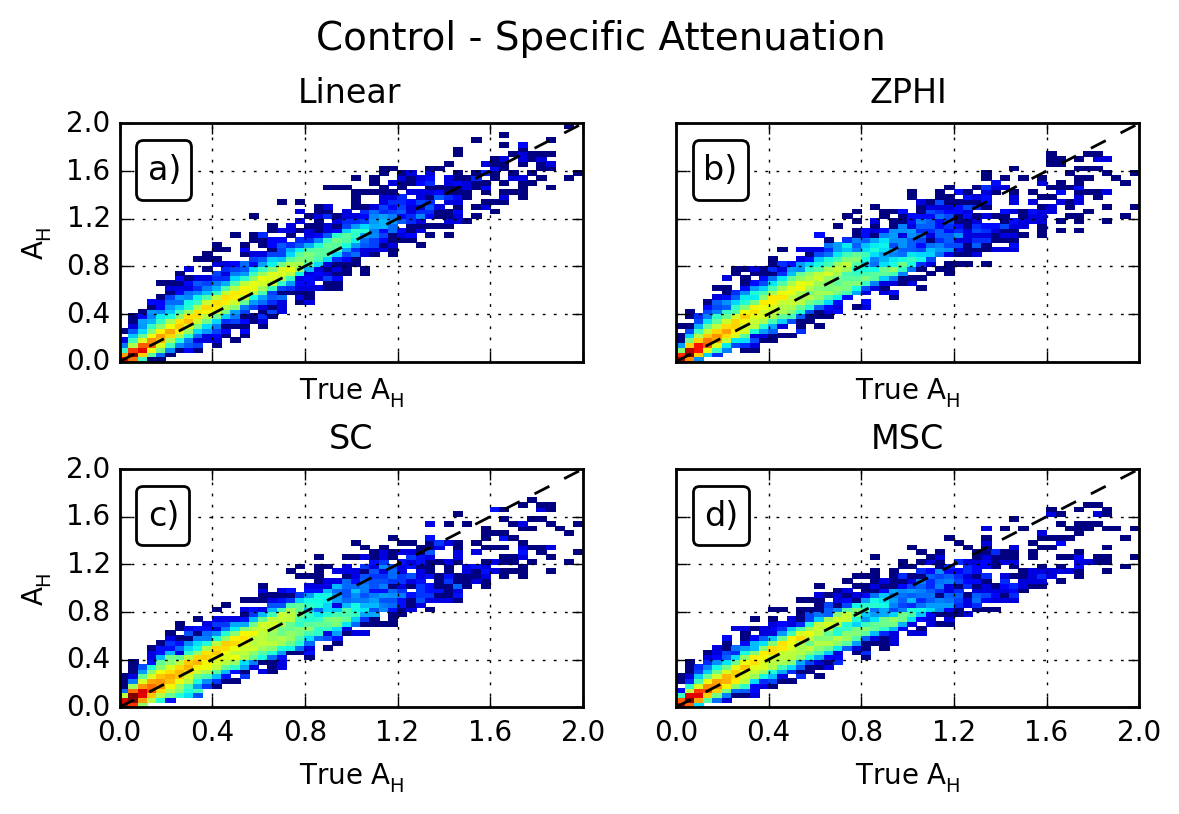
\includegraphics[scale=0.7]{figures/C_Control_Specific_Attenuation_H_scatter}
    \end{center}
\end{frame}

\begin{frame}
    \begin{center}
        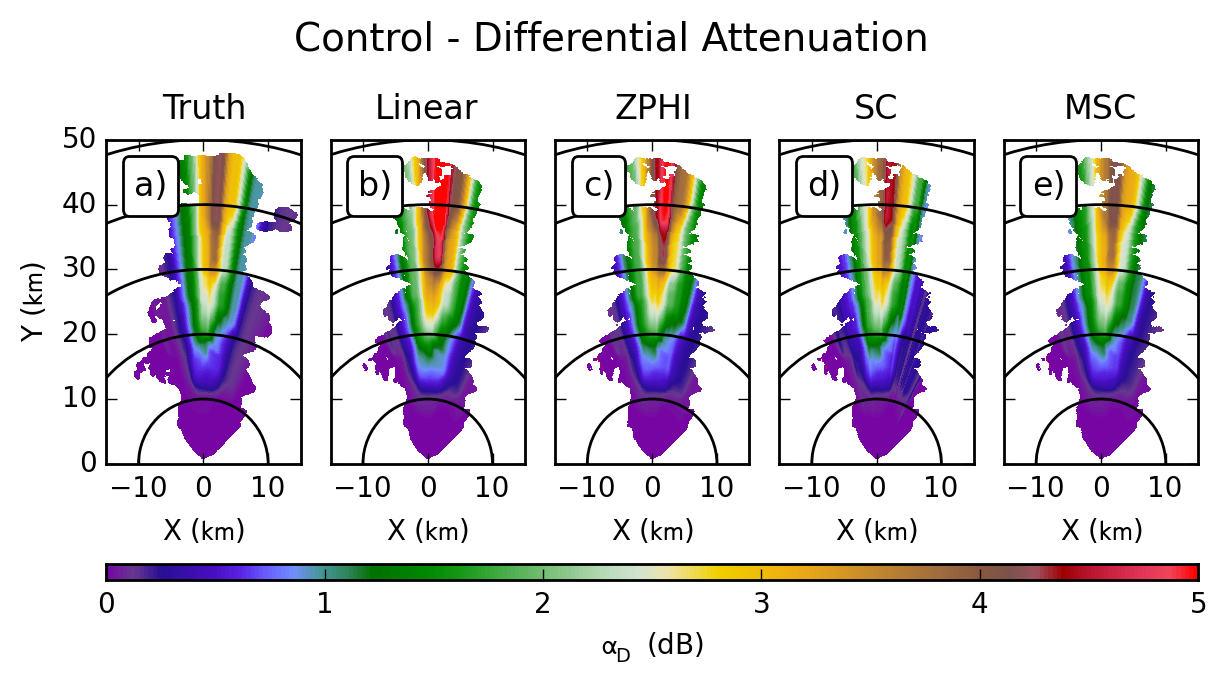
\includegraphics[scale=0.7]{figures/C_Control_Differential_Attenuation}
    \end{center}
\end{frame}

\begin{frame}
    \begin{center}
        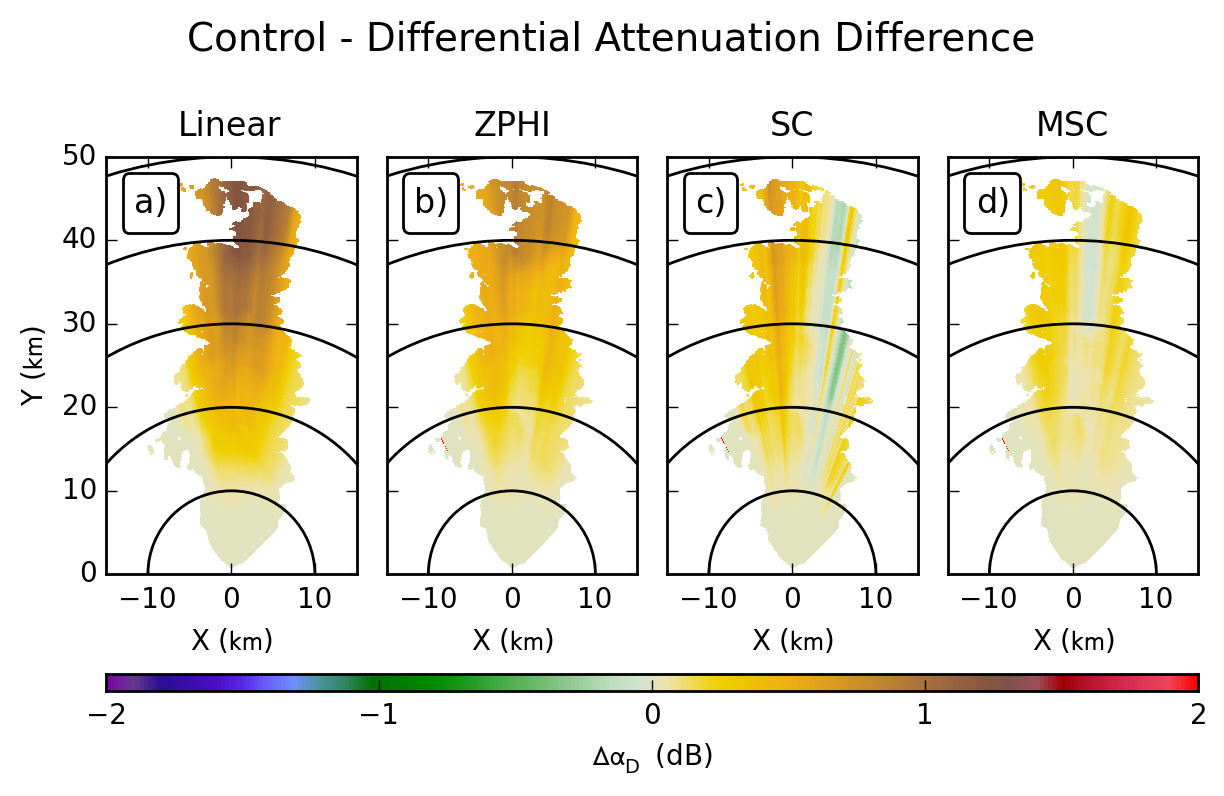
\includegraphics[scale=0.7]{figures/C_Control_Differential_Attenuation_Difference}
    \end{center}
\end{frame}

\begin{frame}
    \begin{center}
        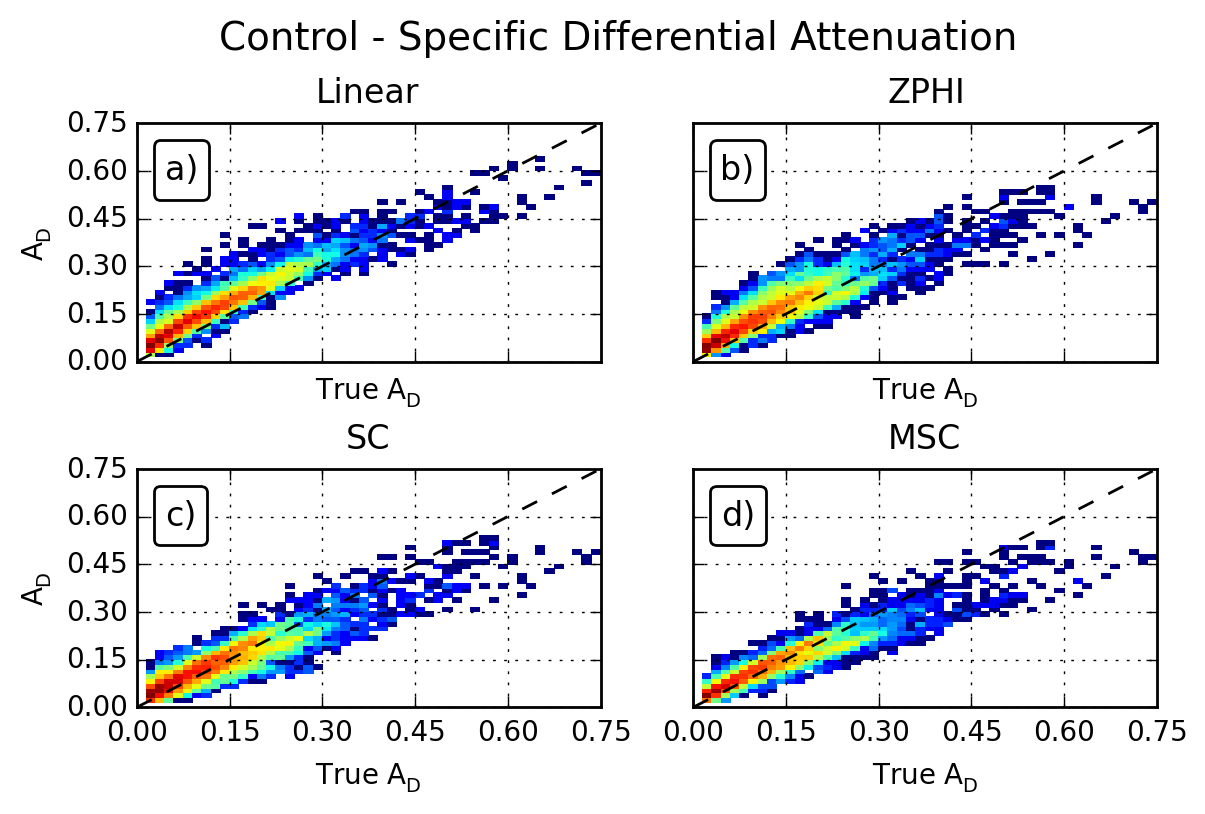
\includegraphics[scale=0.7]{figures/C_Control_Specific_Differential_Attenuation_scatter}
    \end{center}
\end{frame}

\subsubsection{Temperature}
\begin{frame}
	\frametitle{Temperature}
	\begin{center}
	    \begin{tabular}{ | l | l | }
	        \hline
	        Temperature & Model (\SI{295}{\kelvin}) \\
	        Drop Shape Model & Brandes \\
	        Wavelength & \SI{5.5}{\centi\meter}, \SI{3.21}{\centi\meter} \\
			\hline
	    \end{tabular}
	\end{center}	
\end{frame}

\begin{frame}
    \begin{center}
        \includegraphics<1>[scale=0.7]{figures/C_Temperature_Attenuation_Difference_H}
        \includegraphics<2>[scale=0.7]{figures/C_Control_Attenuation_Difference_H}
    \end{center}
\end{frame}

\begin{frame}
    \begin{center}
        \includegraphics<1>[scale=0.7]{figures/C_Temperature_Specific_Attenuation_H_scatter}
        \includegraphics<2>[scale=0.7]{figures/C_Control_Specific_Attenuation_H_scatter}
    \end{center}
\end{frame}

\begin{frame}
    \begin{center}
        \includegraphics<1>[scale=0.7]{figures/C_Temperature_Differential_Attenuation_Difference}
        \includegraphics<2>[scale=0.7]{figures/C_Control_Differential_Attenuation_Difference}
    \end{center}
\end{frame}

\begin{frame}
    \begin{center}
        \includegraphics<1>[scale=0.7]{figures/C_Temperature_Specific_Differential_Attenuation_scatter}
        \includegraphics<2>[scale=0.7]{figures/C_Control_Specific_Differential_Attenuation_scatter}
    \end{center}
\end{frame}

\subsubsection{Wavelength}
\begin{frame}
	\frametitle{Wavelength}
	\begin{center}
	    \begin{tabular}{ | l | l | }
	        \hline
	        Temperature & \SI{283}{\kelvin} \\
	        Drop Shape Model & Brandes \\
	        Wavelength & \SI{5.0}{\centi\meter}, \SI{3.0}{\centi\meter} \\
			\hline
	    \end{tabular}
	\end{center}	
\end{frame}

\begin{frame}
    \begin{center}
        \includegraphics<1>[scale=0.7]{figures/C_Wavelength_Attenuation_Difference_H}
        \includegraphics<2>[scale=0.7]{figures/C_Control_Attenuation_Difference_H}
    \end{center}
\end{frame}

\begin{frame}
    \begin{center}
        \includegraphics<1>[scale=0.7]{figures/C_Wavelength_Specific_Attenuation_H_scatter}
        \includegraphics<2>[scale=0.7]{figures/C_Control_Specific_Attenuation_H_scatter}
    \end{center}
\end{frame}

\begin{frame}
    \begin{center}
        \includegraphics<1>[scale=0.7]{figures/C_Wavelength_Differential_Attenuation_Difference}
        \includegraphics<2>[scale=0.7]{figures/C_Control_Differential_Attenuation_Difference}
    \end{center}
\end{frame}

\begin{frame}
    \begin{center}
        \includegraphics<1>[scale=0.7]{figures/C_Wavelength_Specific_Differential_Attenuation_scatter}
        \includegraphics<2>[scale=0.7]{figures/C_Control_Specific_Differential_Attenuation_scatter}
    \end{center}
\end{frame}

\begin{frame}
    \frametitle{Summary: Bias at C-band for Horizontal Polarization (\si{dB\per \kilo\meter})}
    \begin{center}
        \begin{tabular}{| c | c | c | c | c |}
            \hline
            Experiment & Linear & ZPHI & SC & MSC \\
            \hline
            \hline
            Control & 0.0310 & 0.0281 & 0.0074 & -0.0009 \\
            Canting & 0.0465 & 0.0432 & 0.0082 & -0.0009 \\
            Shape & 0.1191 & 0.1171 & 0.0170 & -0.0088 \\
            Temperature & 0.1009 & 0.0968 & 0.0087 & -0.0009 \\
            Wavelength & -0.0629 & -0.0641 & 0.0076 & 0.0013 \\
            Combined & 0.1335 & 0.1311 & 0.0221 & -0.0104 \\
            \hline
        \end{tabular}
    \end{center}
\end{frame}

\begin{frame}
    \frametitle{Summary: Bias at C-band for Differential Polarization (\si{dB\per \kilo\meter})}
    \begin{center}
        \begin{tabular}{| c | c | c | c | c |}
            \hline
            Experiment & Linear & ZPHI & SC & MSC \\
            \hline
            \hline
            Control & 0.0410 & 0.0287 & 0.0091 & 0.0064 \\
            Canting & 0.0430 & 0.0304 & 0.0098 & 0.0077 \\
            Shape & 0.0683 & 0.0535 & 0.0087 & -0.0082 \\
            Temperature & 0.0540 & 0.0392 & 0.0081 & 0.0118 \\
            Wavelength & 0.0124 & 0.0010 & 0.0099 & 0.0068 \\
            Combined & 0.0512 & 0.0375 & 0.0119 & -0.0088 \\
            \hline
        \end{tabular}
    \end{center}
\end{frame}

\begin{frame}
    \frametitle{Summary: Bias at X-band for Horizontal Polarization (\si{dB\per \kilo\meter})}
    \begin{center}
        \begin{tabular}{| c | c | c | c | c |}
            \hline
            Experiment & Linear & ZPHI & SC & MSC \\
            \hline
            \hline
            Control & 0.0237 & -0.0327 & 0.0151 & 0.0079 \\
            Canting & 0.0960 & 0.0330 & 0.0185 & 0.0096 \\
            Shape & 0.4642 & 0.3904 & 0.0334 & 0.0360 \\
            Temperature & -0.0239 & -0.0773 & 0.0174 & 0.0178 \\
            Wavelength & -0.1385 & -0.1923 & 0.0003 & -0.0077 \\
            Combined & 0.3420 & 0.2355 & -0.0041 & -0.0144 \\
            \hline
        \end{tabular}
    \end{center}
\end{frame}

\begin{frame}
    \frametitle{Summary: Bias at X-band for Differential Polarization (\si{dB\per \kilo\meter})}
    \begin{center}
        \begin{tabular}{| c | c | c | c | c |}
            \hline
            Experiment & Linear & ZPHI & SC & MSC \\
            \hline
            \hline
            Control & 0.0384 & 0.0063 & 0.0106 & 0.0216 \\
            Canting & 0.0404 & 0.0182 & 0.0107 & 0.0220 \\
            Shape & 0.0841 & 0.1683 & 0.0116 & 0.0259 \\
            Temperature & 0.0215 & -0.0067 & 0.0086 & 0.0184 \\
            Wavelength & 0.0220 & -0.0168 & 0.0009 & 0.0109 \\
            Combined & 0.0499 & 0.0419 & -0.0011 & 0.0081 \\
            \hline
        \end{tabular}
    \end{center}
\end{frame}

\subsection{Spatial Errors}
\begin{frame}
	\frametitle{Experimental Configuration}
	\begin{center}
	    \begin{tabular}{ | l | l | }
	        \hline
	        Antenna gain & \SI{45.5}{dB} \\
	        Peak power & \SI{250}{\kilo\watt} \\
	        First range gate & \SI{500}{\meter} \\
	        Noise power & \SI{-113}{dBm} \\
	        Elevation & \SI{0.5}{\degree} \\
	        PRT & \SI{0.667}{\milli\second} \\
	        Canting Width & \num{10} \\
	        Wavelength & \SI{5.5}{\centi\meter}, \SI{3.21}{\centi\meter} \\
	        Temperature & \SI{283}{\kelvin} \\
	        Shape Model & Brandes \\
	        Rotation Rate & \SI{20}{\degree\per\second} \\
	        \hline
	    \end{tabular}
	\end{center}
\end{frame}

\subsubsection{Radial Width}
\begin{frame}
	\frametitle{Radial Width}
	\begin{center}
	    \begin{tabular}{ | l | l | }
	        \hline
	        Radial Spacing & \SI{2.0}{\degree} \\
	        \SI{3}{dB} Beamwidth & \SI{2.0}{\degree} \\
	        Gate Width & \SI{125}{\meter} \\
			\hline
	    \end{tabular}
	\end{center}	
\end{frame}

\begin{frame}
    \begin{center}
        \includegraphics<1>[scale=0.7]{figures/spatial/C_RadialWidth_Attenuation_Difference_H}
        \includegraphics<2>[scale=0.7]{figures/spatial/C_Control_Attenuation_Difference_H}
    \end{center}
\end{frame}

\begin{frame}
    \begin{center}
        \includegraphics<1>[scale=0.7]{figures/spatial/C_RadialWidth_Specific_Attenuation_H_scatter}
        \includegraphics<2>[scale=0.7]{figures/spatial/C_Control_Specific_Attenuation_H_scatter}
    \end{center}
\end{frame}

\begin{frame}
    \begin{center}
        \includegraphics<1>[scale=0.7]{figures/spatial/C_RadialWidth_Differential_Attenuation_Difference}
        \includegraphics<2>[scale=0.7]{figures/spatial/C_Control_Differential_Attenuation_Difference}
    \end{center}
\end{frame}

\begin{frame}
    \begin{center}
        \includegraphics<1>[scale=0.7]{figures/spatial/C_RadialWidth_Specific_Differential_Attenuation_scatter}
        \includegraphics<2>[scale=0.7]{figures/spatial/C_Control_Specific_Differential_Attenuation_scatter}
    \end{center}
\end{frame}

\subsubsection{Range Resolution}
\begin{frame}
	\frametitle{Range Resolution}
	\begin{center}
	    \begin{tabular}{ | l | l | }
	        \hline
	        Radial Spacing & \SI{1.0}{\degree} \\
	        \SI{3}{dB} Beamwidth & \SI{1.0}{\degree} \\
	        Gate Width & \SI{250}{\meter} \\
			\hline
	    \end{tabular}
	\end{center}	
\end{frame}

\begin{frame}
    \begin{center}
        \includegraphics<1>[scale=0.7]{figures/spatial/C_RangeResolution_Attenuation_Difference_H}
        \includegraphics<2>[scale=0.7]{figures/spatial/C_Control_Attenuation_Difference_H}
    \end{center}
\end{frame}

\begin{frame}
    \begin{center}
        \includegraphics<1>[scale=0.7]{figures/spatial/C_RangeResolution_Specific_Attenuation_H_scatter}
        \includegraphics<2>[scale=0.7]{figures/spatial/C_Control_Specific_Attenuation_H_scatter}
    \end{center}
\end{frame}

\begin{frame}
    \begin{center}
        \includegraphics<1>[scale=0.7]{figures/spatial/C_RangeResolution_Differential_Attenuation_Difference}
        \includegraphics<2>[scale=0.7]{figures/spatial/C_Control_Differential_Attenuation_Difference}
    \end{center}
\end{frame}

\begin{frame}
    \begin{center}
        \includegraphics<1>[scale=0.7]{figures/spatial/C_RangeResolution_Specific_Differential_Attenuation_scatter}
        \includegraphics<2>[scale=0.7]{figures/spatial/C_Control_Specific_Differential_Attenuation_scatter}
    \end{center}
\end{frame}

\subsubsection{Combined}
\begin{frame}
	\frametitle{Combined: Worst Case}
	\begin{center}
	    \begin{tabular}{ | l | l | }
	        \hline
	        Radial Spacing & \SI{1.0}{\degree} \\
	        \SI{3}{dB} Beamwidth & \SI{1.0}{\degree} \\
	        Gate Width & \SI{125}{\meter} \\
	        Temperature & Model (\SI{295}{\kelvin}) \\
	        Drop Shape Model & Pruppacher \\
			\hline
	    \end{tabular}
	\end{center}	
\end{frame}

\begin{frame}
    \begin{center}
        \includegraphics<1>[scale=0.7]{figures/spatial/C_Combined_Attenuation_H}
        \includegraphics<2>[scale=0.7]{figures/spatial/C_Control_Attenuation_H}
    \end{center}
\end{frame}

\begin{frame}
    \begin{center}
        \includegraphics<1>[scale=0.7]{figures/spatial/C_Combined_Attenuation_Difference_H}
        \includegraphics<2>[scale=0.7]{figures/spatial/C_Control_Attenuation_Difference_H}
    \end{center}
\end{frame}

\begin{frame}
    \begin{center}
        \includegraphics<1>[scale=0.7]{figures/spatial/C_Combined_Specific_Attenuation_H_scatter}
        \includegraphics<2>[scale=0.7]{figures/spatial/C_Control_Specific_Attenuation_H_scatter}
    \end{center}
\end{frame}

\begin{frame}
    \begin{center}
        \includegraphics<1>[scale=0.7]{figures/spatial/C_Combined_Differential_Attenuation}
        \includegraphics<2>[scale=0.7]{figures/spatial/C_Control_Differential_Attenuation}
    \end{center}
\end{frame}

\begin{frame}
    \begin{center}
        \includegraphics<1>[scale=0.7]{figures/spatial/C_Combined_Differential_Attenuation_Difference}
        \includegraphics<2>[scale=0.7]{figures/spatial/C_Control_Differential_Attenuation_Difference}
    \end{center}
\end{frame}

\begin{frame}
    \begin{center}
        \includegraphics<1>[scale=0.7]{figures/spatial/C_Combined_Specific_Differential_Attenuation_scatter}
        \includegraphics<2>[scale=0.7]{figures/spatial/C_Control_Specific_Differential_Attenuation_scatter}
    \end{center}
\end{frame}

\begin{frame}
    \frametitle{Summary: Bias at C-band for Horizontal Polarization (\si{dB\per \kilo\meter})}
    \begin{center}
        \begin{tabular}{| c | c | c | c | c |}
            \hline
            Experiment & Linear & ZPHI & SC & MSC \\
            \hline
            \hline
            Control & 0.0314 & 0.0286 & 0.0059 & -0.0025 \\
            Beamwidth & 0.0322 & 0.0293 & 0.0049 & 0.0065 \\
            Radial Width & 0.0334 & 0.0306 & 0.0071 & 0.0035 \\
            Range Resolution & 0.0313 & 0.0284 & 0.0021 & -0.0054 \\
            Sidelobe & 0.0314 & 0.0286 & 0.0059 & 0.0015 \\
            Combined & 0.1911 & 0.1877 & 0.0172 & 0.0035 \\
            \hline
        \end{tabular}
    \end{center}
\end{frame}

\begin{frame}
    \frametitle{Summary: Bias at C-band for Differential Polarization (\si{dB\per \kilo\meter})}
    \begin{center}
        \begin{tabular}{| c | c | c | c | c |}
            \hline
            Experiment & Linear & ZPHI & SC & MSC \\
            \hline
            \hline
            Control & 0.0407 & 0.0285 & 0.0079 & -0.0014 \\
            Beamwidth & 0.0403 & 0.0278 & 0.0072 & 0.0148 \\
            Radial Width & 0.0398 & 0.0274 & 0.0069 & 0.0002 \\
            Range Resolution & 0.0392 & 0.0280 & 0.0073 & 0.0034 \\
            Sidelobe & 0.0407 & 0.0285 & 0.0080 & 0.0053 \\
            Combined & 0.0843 & 0.0653 & 0.0062 & 0.0022 \\
            \hline
        \end{tabular}
    \end{center}
\end{frame}

\begin{frame}
    \frametitle{Summary: Bias at X-band for Horizontal Polarization (\si{dB\per \kilo\meter})}
    \begin{center}
        \begin{tabular}{| c | c | c | c | c |}
            \hline
            Experiment & Linear & ZPHI & SC & MSC \\
            \hline
            \hline
            Control & 0.0530 & -0.0034 & 0.0365 & 0.0991 \\
            Beamwidth & 0.1009 & 0.0454 & 0.0687 & 0.2072 \\
            Radial Width & 0.1331 & 0.0743 & 0.0910 & 0.1697 \\
            Range Resolution & 0.0507 & -0.0048 & 0.0258 & 0.0264 \\
            Sidelobe & 0.0531 & -0.0029 & 0.0372 & 0.0545 \\
            Combined & 0.4650 & 0.3973 & 0.0551 & 0.0690 \\
            \hline
        \end{tabular}
    \end{center}
\end{frame}

\begin{frame}
    \frametitle{Summary: Bias at X-band for Differential Polarization (\si{dB\per \kilo\meter})}
    \begin{center}
        \begin{tabular}{| c | c | c | c | c |}
            \hline
            Experiment & Linear & ZPHI & SC & MSC \\
            \hline
            \hline
            Control & 0.0394 & 0.0098 & 0.0098 & 0.1006 \\
            Beamwidth & 0.0407 & 0.0129 & 0.0075 & 0.1524 \\
            Radial Width & 0.0416 & 0.0127 & 0.0046 & 0.0779 \\
            Range Resolution & 0.0378 & 0.0085 & 0.0051 & 0.0187 \\
            Sidelobe & 0.0394 & 0.0067 & 0.0060 & 0.0388 \\
            Combined & 0.0705 & 0.1441 & 0.0129 & 0.0252 \\
            \hline
        \end{tabular}
    \end{center}
\end{frame}

\section{Conclusions}
\stepcounter{subsection}
\begin{frame}[<+->]
	\frametitle{Conclusions}
	\begin{itemize}
		\item Combination of approaches of Mischenko (1999) and Galati (1995)
		produces useful and realistic synthetic time series radar data
		\item The performance of the linear $\Phi_{DP}$ and ZPHI algorithms depend heavily upon having coefficients
		that reflect the true scattering physics
		\item Correction for differential attenuation performs worse across all the algorithms, at least relative to the expected $Z_{DR}$ values
		\item For linear $\Phi_{DP}$ and ZPHI, simply using coefficients to the wave-band of interest can cause non-negligible error
	\end{itemize}
\end{frame}

\begin{frame}[<+->]
	\frametitle{Conclusions}
	\begin{itemize}
		\item Algorithm error characteristics are insensitive to (reasonable) spatial sampling configuration
		\item Errors caused by differences between assumed and actual physics are dominant
		\item The self-consistent versions of ZPHI perform well overall at removing biases due to changing physics; however this comes
		at a cost of some rays that have increased error
		\item The Modified Self-Consistent method, using the median coefficient,
		often succeeds at producing better results....
		\item ...at the cost of reduced performance in a few cases.
	\end{itemize}
\end{frame}

\begin{frame}
	\frametitle{Thanks}
	\begin{itemize}
		\item Dr. Ted Mansell for performing the model simulation
		\item The NumPy, SciPy, and Matplotlib Python projects that makes this possible
		\item All of my officemates over the years
		\item Dr. Mike Biggerstaff, my advisor, for putting up with me all these years
	\end{itemize}
	\begin{center}
		\large{Questions?}
	\end{center}
\end{frame}

\appendix
\newcounter{finalframe}
\setcounter{finalframe}{\value{framenumber}}
\section{Backup}
\begin{frame}
	\begin{center}
		Backup Slides
	\end{center}
\end{frame}

\subsection{Model Errors}
\subsubsection{Control}
\begin{frame}
    \begin{center}
        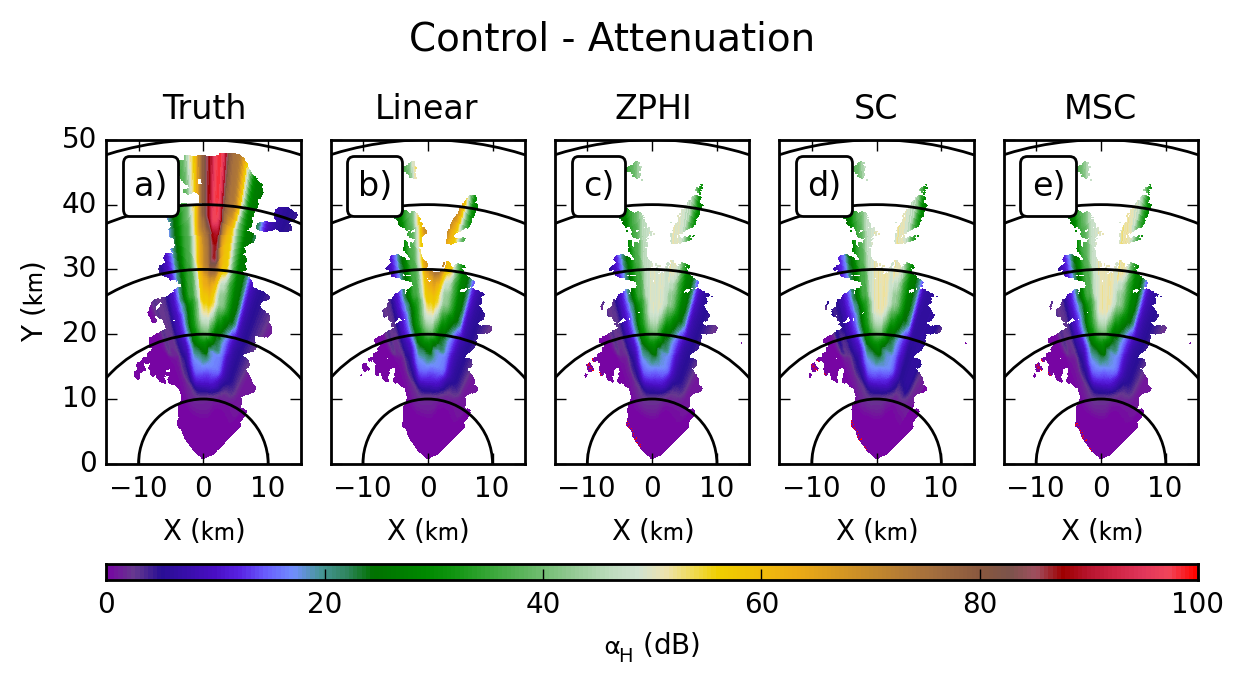
\includegraphics[scale=0.7]{figures/X_Control_Attenuation_H}
    \end{center}
\end{frame}

\begin{frame}
    \begin{center}
        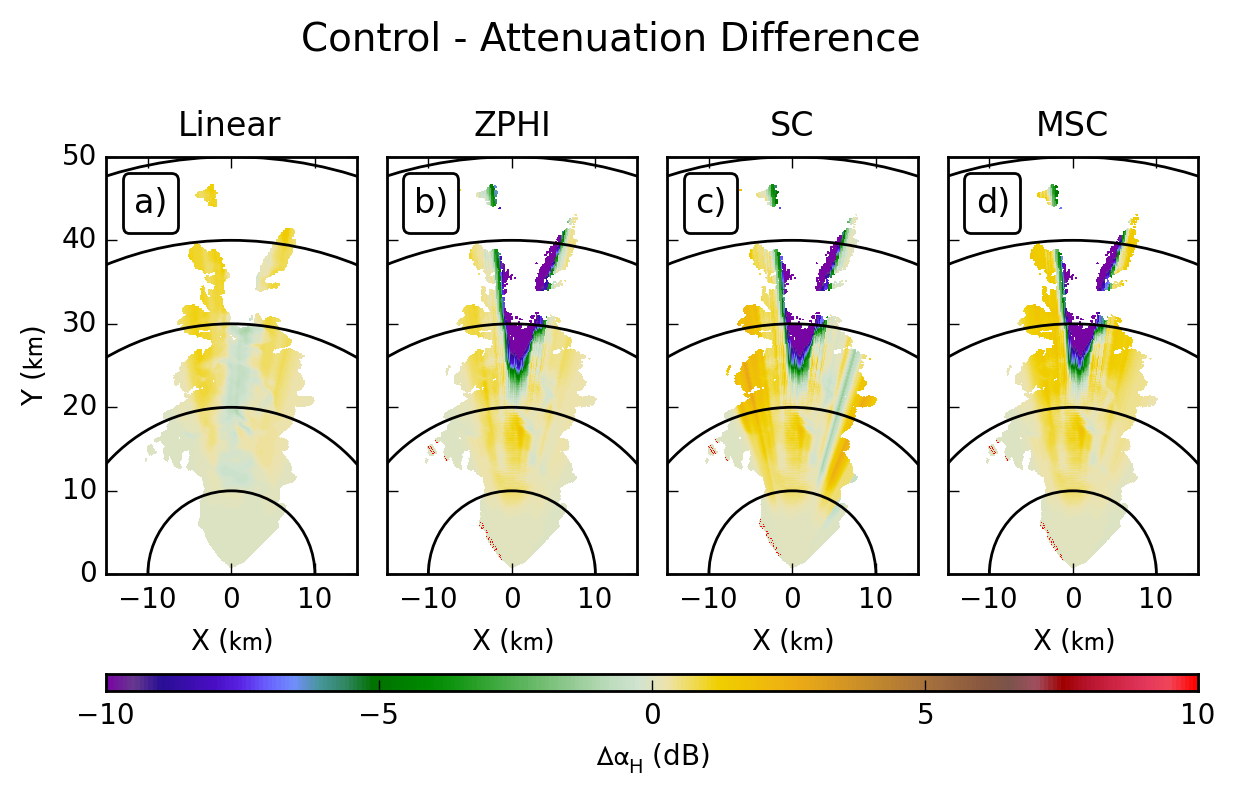
\includegraphics[scale=0.7]{figures/X_Control_Attenuation_Difference_H}
    \end{center}
\end{frame}

\begin{frame}
    \begin{center}
        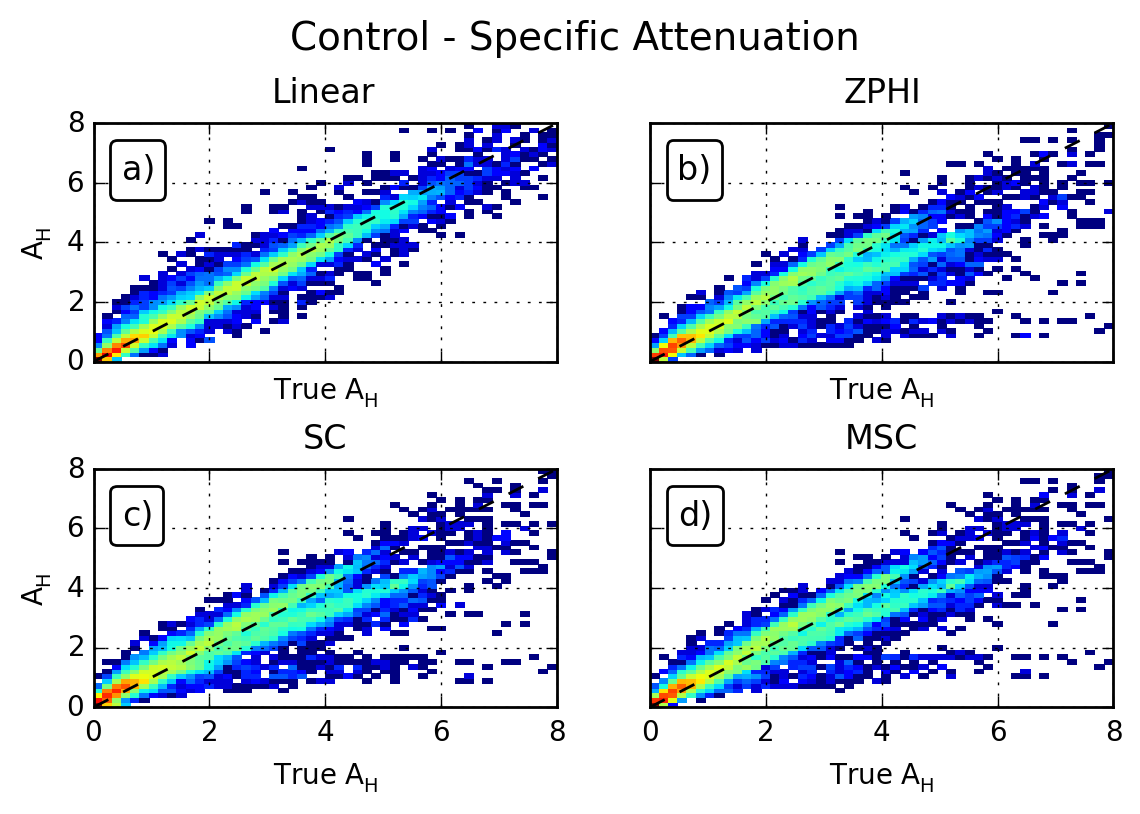
\includegraphics[scale=0.7]{figures/X_Control_Specific_Attenuation_H_scatter}
    \end{center}
\end{frame}

\begin{frame}
    \begin{center}
        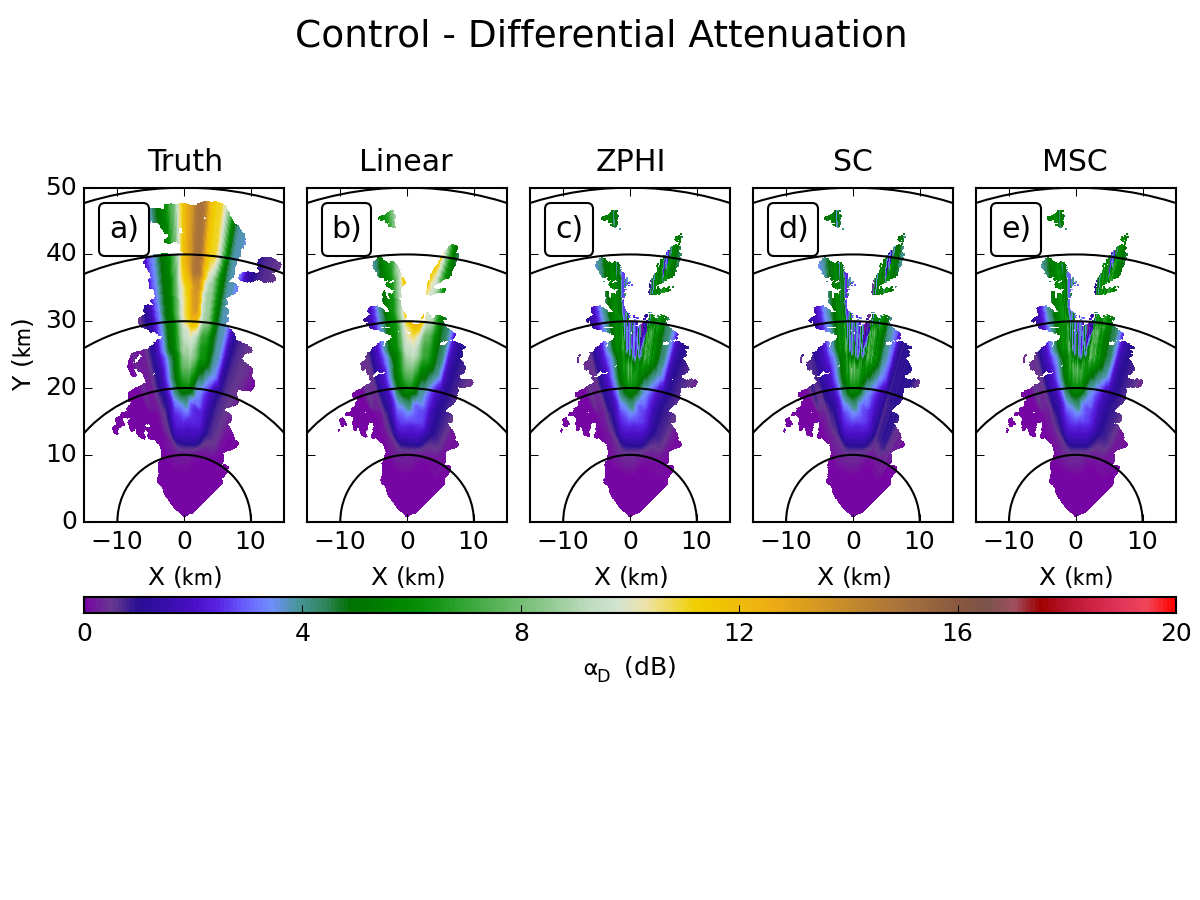
\includegraphics[scale=0.7]{figures/X_Control_Differential_Attenuation}
    \end{center}
\end{frame}

\begin{frame}
    \begin{center}
        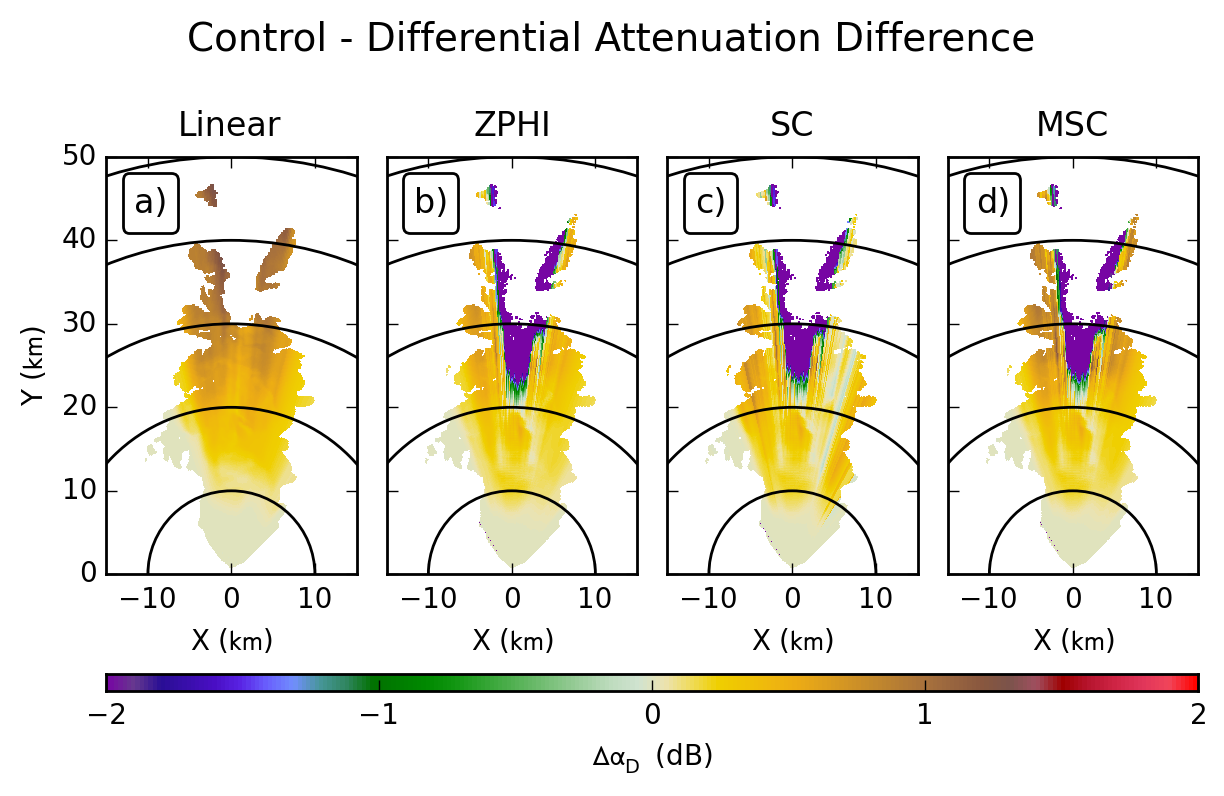
\includegraphics[scale=0.7]{figures/X_Control_Differential_Attenuation_Difference}
    \end{center}
\end{frame}

\begin{frame}
    \begin{center}
        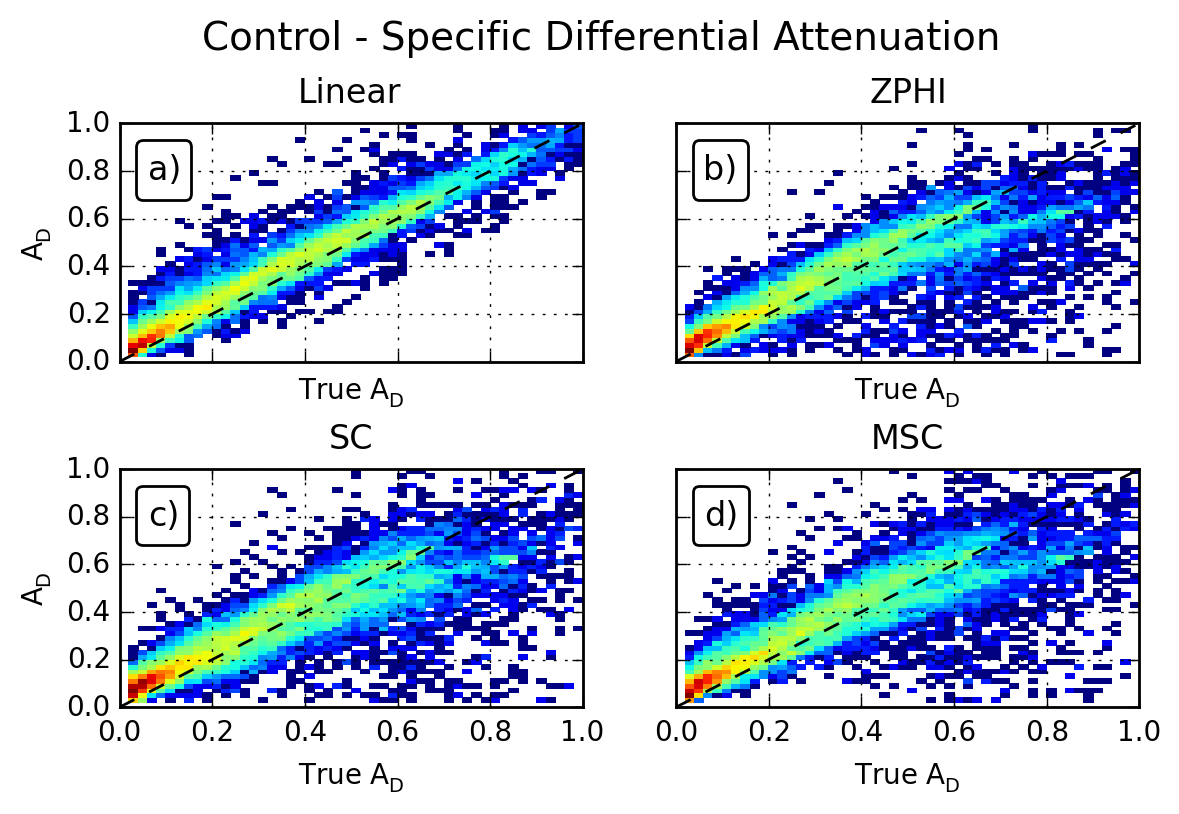
\includegraphics[scale=0.7]{figures/X_Control_Specific_Differential_Attenuation_scatter}
    \end{center}
\end{frame}

\subsubsection{Canting}
\begin{frame}
    \begin{center}
        \includegraphics<1>[scale=0.7]{figures/C_Canting_Attenuation_H}
        \includegraphics<2>[scale=0.7]{figures/C_Control_Attenuation_H}
    \end{center}
\end{frame}

\begin{frame}
    \begin{center}
        \includegraphics<1>[scale=0.7]{figures/C_Canting_Attenuation_Difference_H}
        \includegraphics<2>[scale=0.7]{figures/C_Control_Attenuation_Difference_H}
    \end{center}
\end{frame}

\begin{frame}
    \begin{center}
        \includegraphics<1>[scale=0.7]{figures/C_Canting_Specific_Attenuation_H_scatter}
        \includegraphics<2>[scale=0.7]{figures/C_Control_Specific_Attenuation_H_scatter}
    \end{center}
\end{frame}

\begin{frame}
    \begin{center}
        \includegraphics<1>[scale=0.7]{figures/C_Canting_Differential_Attenuation}
        \includegraphics<2>[scale=0.7]{figures/C_Control_Differential_Attenuation}
    \end{center}
\end{frame}

\begin{frame}
    \begin{center}
        \includegraphics<1>[scale=0.7]{figures/C_Canting_Differential_Attenuation_Difference}
        \includegraphics<2>[scale=0.7]{figures/C_Control_Differential_Attenuation_Difference}
    \end{center}
\end{frame}

\begin{frame}
    \begin{center}
        \includegraphics<1>[scale=0.7]{figures/C_Canting_Specific_Differential_Attenuation_scatter}
        \includegraphics<2>[scale=0.7]{figures/C_Control_Specific_Differential_Attenuation_scatter}
    \end{center}
\end{frame}

\begin{frame}
    \begin{center}
        \includegraphics<1>[scale=0.7]{figures/X_Canting_Attenuation_H}
        \includegraphics<2>[scale=0.7]{figures/X_Control_Attenuation_H}
    \end{center}
\end{frame}

\begin{frame}
    \begin{center}
        \includegraphics<1>[scale=0.7]{figures/X_Canting_Attenuation_Difference_H}
        \includegraphics<2>[scale=0.7]{figures/X_Control_Attenuation_Difference_H}
    \end{center}
\end{frame}

\begin{frame}
    \begin{center}
        \includegraphics<1>[scale=0.7]{figures/X_Canting_Specific_Attenuation_H_scatter}
        \includegraphics<2>[scale=0.7]{figures/X_Control_Specific_Attenuation_H_scatter}
    \end{center}
\end{frame}

\begin{frame}
    \begin{center}
        \includegraphics<1>[scale=0.7]{figures/X_Canting_Differential_Attenuation}
        \includegraphics<2>[scale=0.7]{figures/X_Control_Differential_Attenuation}
    \end{center}
\end{frame}

\begin{frame}
    \begin{center}
        \includegraphics<1>[scale=0.7]{figures/X_Canting_Differential_Attenuation_Difference}
        \includegraphics<2>[scale=0.7]{figures/X_Control_Differential_Attenuation_Difference}
    \end{center}
\end{frame}

\begin{frame}
    \begin{center}
        \includegraphics<1>[scale=0.7]{figures/X_Canting_Specific_Differential_Attenuation_scatter}
        \includegraphics<2>[scale=0.7]{figures/X_Control_Specific_Differential_Attenuation_scatter}
    \end{center}
\end{frame}

\subsubsection{Shape}
\begin{frame}
	\frametitle{Shape}
	\begin{center}
	    \begin{tabular}{ | l | l | }
	        \hline
	        Temperature & \SI{283}{\kelvin} \\
	        Drop Shape Model & Pruppacher \\
	        Wavelength & \SI{5.5}{\centi\meter}, \SI{3.21}{\centi\meter} \\
			\hline
	    \end{tabular}
	\end{center}	
\end{frame}

\begin{frame}
    \begin{center}
        \includegraphics<1>[scale=0.7]{figures/C_Shape_Attenuation_H}
        \includegraphics<2>[scale=0.7]{figures/C_Control_Attenuation_H}
    \end{center}
\end{frame}

\begin{frame}
    \begin{center}
        \includegraphics<1>[scale=0.7]{figures/C_Shape_Attenuation_Difference_H}
        \includegraphics<2>[scale=0.7]{figures/C_Control_Attenuation_Difference_H}
    \end{center}
\end{frame}

\begin{frame}
    \begin{center}
        \includegraphics<1>[scale=0.7]{figures/C_Shape_Specific_Attenuation_H_scatter}
        \includegraphics<2>[scale=0.7]{figures/C_Control_Specific_Attenuation_H_scatter}
    \end{center}
\end{frame}

\begin{frame}
    \begin{center}
        \includegraphics<1>[scale=0.7]{figures/C_Shape_Differential_Attenuation}
        \includegraphics<2>[scale=0.7]{figures/C_Control_Differential_Attenuation}
    \end{center}
\end{frame}

\begin{frame}
    \begin{center}
        \includegraphics<1>[scale=0.7]{figures/C_Shape_Differential_Attenuation_Difference}
        \includegraphics<2>[scale=0.7]{figures/C_Control_Differential_Attenuation_Difference}
    \end{center}
\end{frame}

\begin{frame}
    \begin{center}
        \includegraphics<1>[scale=0.7]{figures/C_Shape_Specific_Differential_Attenuation_scatter}
        \includegraphics<2>[scale=0.7]{figures/C_Control_Specific_Differential_Attenuation_scatter}
    \end{center}
\end{frame}

\begin{frame}
    \begin{center}
        \includegraphics<1>[scale=0.7]{figures/X_Shape_Attenuation_H}
        \includegraphics<2>[scale=0.7]{figures/X_Control_Attenuation_H}
    \end{center}
\end{frame}

\begin{frame}
    \begin{center}
        \includegraphics<1>[scale=0.7]{figures/X_Shape_Attenuation_Difference_H}
        \includegraphics<2>[scale=0.7]{figures/X_Control_Attenuation_Difference_H}
    \end{center}
\end{frame}

\begin{frame}
    \begin{center}
        \includegraphics<1>[scale=0.7]{figures/X_Shape_Specific_Attenuation_H_scatter}
        \includegraphics<2>[scale=0.7]{figures/X_Control_Specific_Attenuation_H_scatter}
    \end{center}
\end{frame}

\begin{frame}
    \begin{center}
        \includegraphics<1>[scale=0.7]{figures/X_Shape_Differential_Attenuation}
        \includegraphics<2>[scale=0.7]{figures/X_Control_Differential_Attenuation}
    \end{center}
\end{frame}

\begin{frame}
    \begin{center}
        \includegraphics<1>[scale=0.7]{figures/X_Shape_Differential_Attenuation_Difference}
        \includegraphics<2>[scale=0.7]{figures/X_Control_Differential_Attenuation_Difference}
    \end{center}
\end{frame}

\begin{frame}
    \begin{center}
        \includegraphics<1>[scale=0.7]{figures/X_Shape_Specific_Differential_Attenuation_scatter}
        \includegraphics<2>[scale=0.7]{figures/X_Control_Specific_Differential_Attenuation_scatter}
    \end{center}
\end{frame}

\subsubsection{Temperature}
\begin{frame}
    \begin{center}
        \includegraphics<1>[scale=0.7]{figures/C_Temperature_Attenuation_H}
        \includegraphics<2>[scale=0.7]{figures/C_Control_Attenuation_H}
    \end{center}
\end{frame}

\begin{frame}
    \begin{center}
        \includegraphics<1>[scale=0.7]{figures/C_Temperature_Differential_Attenuation}
        \includegraphics<2>[scale=0.7]{figures/C_Control_Differential_Attenuation}
    \end{center}
\end{frame}

\begin{frame}
    \begin{center}
        \includegraphics<1>[scale=0.7]{figures/X_Temperature_Attenuation_H}
        \includegraphics<2>[scale=0.7]{figures/X_Control_Attenuation_H}
    \end{center}
\end{frame}

\begin{frame}
    \begin{center}
        \includegraphics<1>[scale=0.7]{figures/X_Temperature_Attenuation_Difference_H}
        \includegraphics<2>[scale=0.7]{figures/X_Control_Attenuation_Difference_H}
    \end{center}
\end{frame}

\begin{frame}
    \begin{center}
        \includegraphics<1>[scale=0.7]{figures/X_Temperature_Specific_Attenuation_H_scatter}
        \includegraphics<2>[scale=0.7]{figures/X_Control_Specific_Attenuation_H_scatter}
    \end{center}
\end{frame}

\begin{frame}
    \begin{center}
        \includegraphics<1>[scale=0.7]{figures/X_Temperature_Differential_Attenuation}
        \includegraphics<2>[scale=0.7]{figures/X_Control_Differential_Attenuation}
    \end{center}
\end{frame}

\begin{frame}
    \begin{center}
        \includegraphics<1>[scale=0.7]{figures/X_Temperature_Differential_Attenuation_Difference}
        \includegraphics<2>[scale=0.7]{figures/X_Control_Differential_Attenuation_Difference}
    \end{center}
\end{frame}

\begin{frame}
    \begin{center}
        \includegraphics<1>[scale=0.7]{figures/X_Temperature_Specific_Differential_Attenuation_scatter}
        \includegraphics<2>[scale=0.7]{figures/X_Control_Specific_Differential_Attenuation_scatter}
    \end{center}
\end{frame}

\subsubsection{Wavelength}
\begin{frame}
    \begin{center}
        \includegraphics<1>[scale=0.7]{figures/C_Wavelength_Attenuation_H}
        \includegraphics<2>[scale=0.7]{figures/C_Control_Attenuation_H}
    \end{center}
\end{frame}

\begin{frame}
    \begin{center}
        \includegraphics<1>[scale=0.7]{figures/C_Wavelength_Differential_Attenuation}
        \includegraphics<2>[scale=0.7]{figures/C_Control_Differential_Attenuation}
    \end{center}
\end{frame}

\begin{frame}
    \begin{center}
        \includegraphics<1>[scale=0.7]{figures/X_Wavelength_Attenuation_H}
        \includegraphics<2>[scale=0.7]{figures/X_Control_Attenuation_H}
    \end{center}
\end{frame}

\begin{frame}
    \begin{center}
        \includegraphics<1>[scale=0.7]{figures/X_Wavelength_Attenuation_Difference_H}
        \includegraphics<2>[scale=0.7]{figures/X_Control_Attenuation_Difference_H}
    \end{center}
\end{frame}

\begin{frame}
    \begin{center}
        \includegraphics<1>[scale=0.7]{figures/X_Wavelength_Specific_Attenuation_H_scatter}
        \includegraphics<2>[scale=0.7]{figures/X_Control_Specific_Attenuation_H_scatter}
    \end{center}
\end{frame}

\begin{frame}
    \begin{center}
        \includegraphics<1>[scale=0.7]{figures/X_Wavelength_Differential_Attenuation}
        \includegraphics<2>[scale=0.7]{figures/X_Control_Differential_Attenuation}
    \end{center}
\end{frame}

\begin{frame}
    \begin{center}
        \includegraphics<1>[scale=0.7]{figures/X_Wavelength_Differential_Attenuation_Difference}
        \includegraphics<2>[scale=0.7]{figures/X_Control_Differential_Attenuation_Difference}
    \end{center}
\end{frame}

\begin{frame}
    \begin{center}
        \includegraphics<1>[scale=0.7]{figures/X_Wavelength_Specific_Differential_Attenuation_scatter}
        \includegraphics<2>[scale=0.7]{figures/X_Control_Specific_Differential_Attenuation_scatter}
    \end{center}
\end{frame}

\subsubsection{Combined}
\begin{frame}
	\frametitle{Worst Case}
	\begin{center}
	    \begin{tabular}{ | l | l | }
	        \hline
	        Temperature & Model Field (\textasciitilde\SI{293}{\kelvin}) \\
	        Drop Shape Model & Pruppacher \\
	        Wavelength & \SI{5.0}{\centi\meter} \\
			\hline
	    \end{tabular}
	\end{center}	
\end{frame}

\begin{frame}
    \begin{center}
        \includegraphics<1>[scale=0.7]{figures/C_Combined_Attenuation_H}
        \includegraphics<2>[scale=0.7]{figures/C_Control_Attenuation_H}
    \end{center}
\end{frame}

\begin{frame}
    \begin{center}
        \includegraphics<1>[scale=0.7]{figures/C_Combined_Attenuation_Difference_H}
        \includegraphics<2>[scale=0.7]{figures/C_Control_Attenuation_Difference_H}
    \end{center}
\end{frame}

\begin{frame}
    \begin{center}
        \includegraphics<1>[scale=0.7]{figures/C_Combined_Specific_Attenuation_H_scatter}
        \includegraphics<2>[scale=0.7]{figures/C_Control_Specific_Attenuation_H_scatter}
    \end{center}
\end{frame}

\begin{frame}
    \begin{center}
        \includegraphics<1>[scale=0.7]{figures/C_Combined_Differential_Attenuation}
        \includegraphics<2>[scale=0.7]{figures/C_Control_Differential_Attenuation}
    \end{center}
\end{frame}

\begin{frame}
    \begin{center}
        \includegraphics<1>[scale=0.7]{figures/C_Combined_Differential_Attenuation_Difference}
        \includegraphics<2>[scale=0.7]{figures/C_Control_Differential_Attenuation_Difference}
    \end{center}
\end{frame}

\begin{frame}
    \begin{center}
        \includegraphics<1>[scale=0.7]{figures/C_Combined_Specific_Differential_Attenuation_scatter}
        \includegraphics<2>[scale=0.7]{figures/C_Control_Specific_Differential_Attenuation_scatter}
    \end{center}
\end{frame}

\begin{frame}
    \begin{center}
        \includegraphics<1>[scale=0.7]{figures/X_Combined_Attenuation_H}
        \includegraphics<2>[scale=0.7]{figures/X_Control_Attenuation_H}
    \end{center}
\end{frame}

\begin{frame}
    \begin{center}
        \includegraphics<1>[scale=0.7]{figures/X_Combined_Attenuation_Difference_H}
        \includegraphics<2>[scale=0.7]{figures/X_Control_Attenuation_Difference_H}
    \end{center}
\end{frame}

\begin{frame}
    \begin{center}
        \includegraphics<1>[scale=0.7]{figures/X_Combined_Specific_Attenuation_H_scatter}
        \includegraphics<2>[scale=0.7]{figures/X_Control_Specific_Attenuation_H_scatter}
    \end{center}
\end{frame}

\begin{frame}
    \begin{center}
        \includegraphics<1>[scale=0.7]{figures/X_Combined_Differential_Attenuation}
        \includegraphics<2>[scale=0.7]{figures/X_Control_Differential_Attenuation}
    \end{center}
\end{frame}

\begin{frame}
    \begin{center}
        \includegraphics<1>[scale=0.7]{figures/X_Combined_Differential_Attenuation_Difference}
        \includegraphics<2>[scale=0.7]{figures/X_Control_Differential_Attenuation_Difference}
    \end{center}
\end{frame}

\begin{frame}
    \begin{center}
        \includegraphics<1>[scale=0.7]{figures/X_Combined_Specific_Differential_Attenuation_scatter}
        \includegraphics<2>[scale=0.7]{figures/X_Control_Specific_Differential_Attenuation_scatter}
    \end{center}
\end{frame}

\subsubsection{Vertical Channel}
\begin{frame}
    \begin{center}
        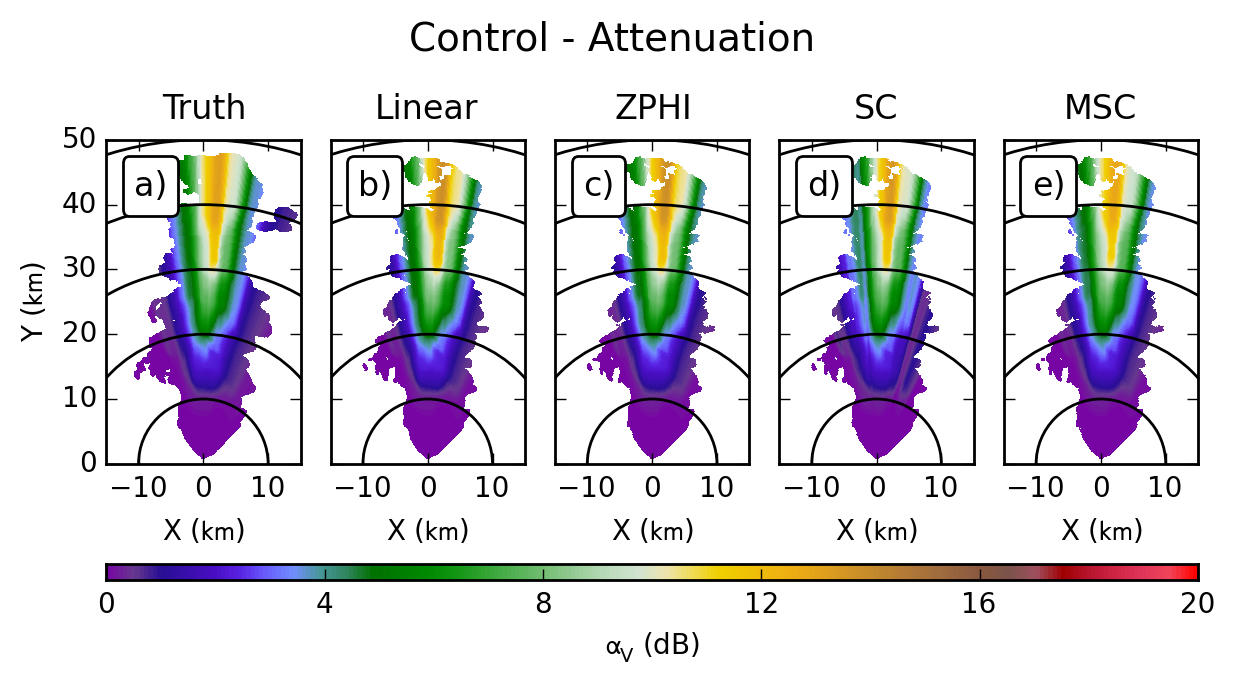
\includegraphics[scale=0.7]{figures/C_Control_Attenuation_V}
    \end{center}
\end{frame}

\begin{frame}
    \begin{center}
        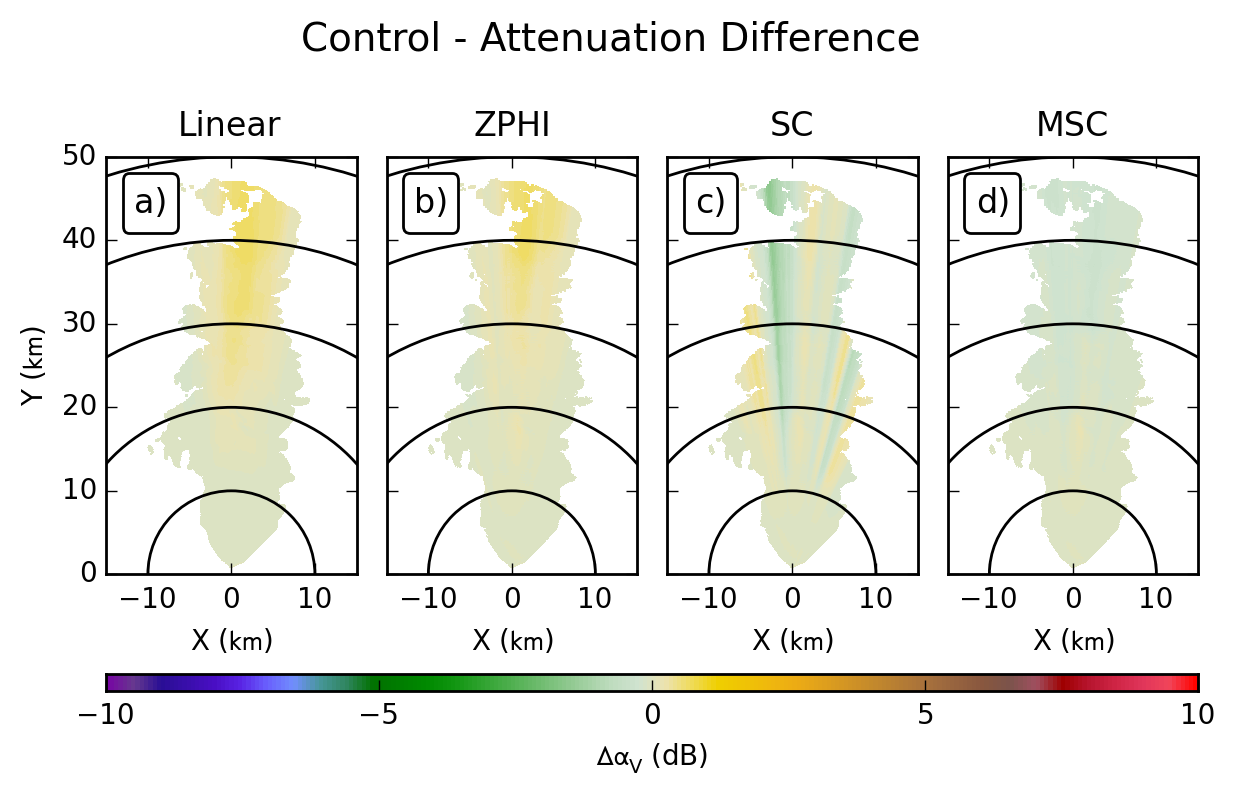
\includegraphics[scale=0.7]{figures/C_Control_Attenuation_Difference_V}
    \end{center}
\end{frame}

\begin{frame}
    \begin{center}
        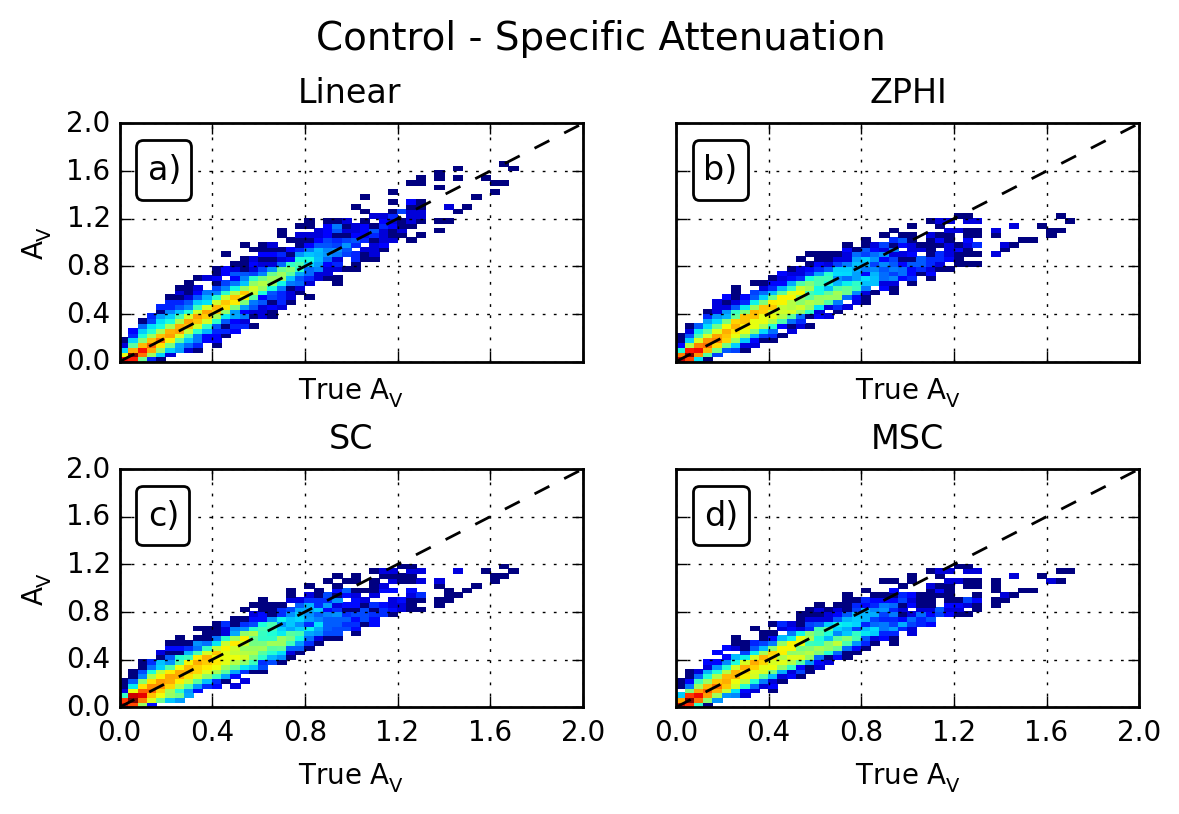
\includegraphics[scale=0.7]{figures/C_Control_Specific_Attenuation_V_scatter}
    \end{center}
\end{frame}

\begin{frame}
    \begin{center}
        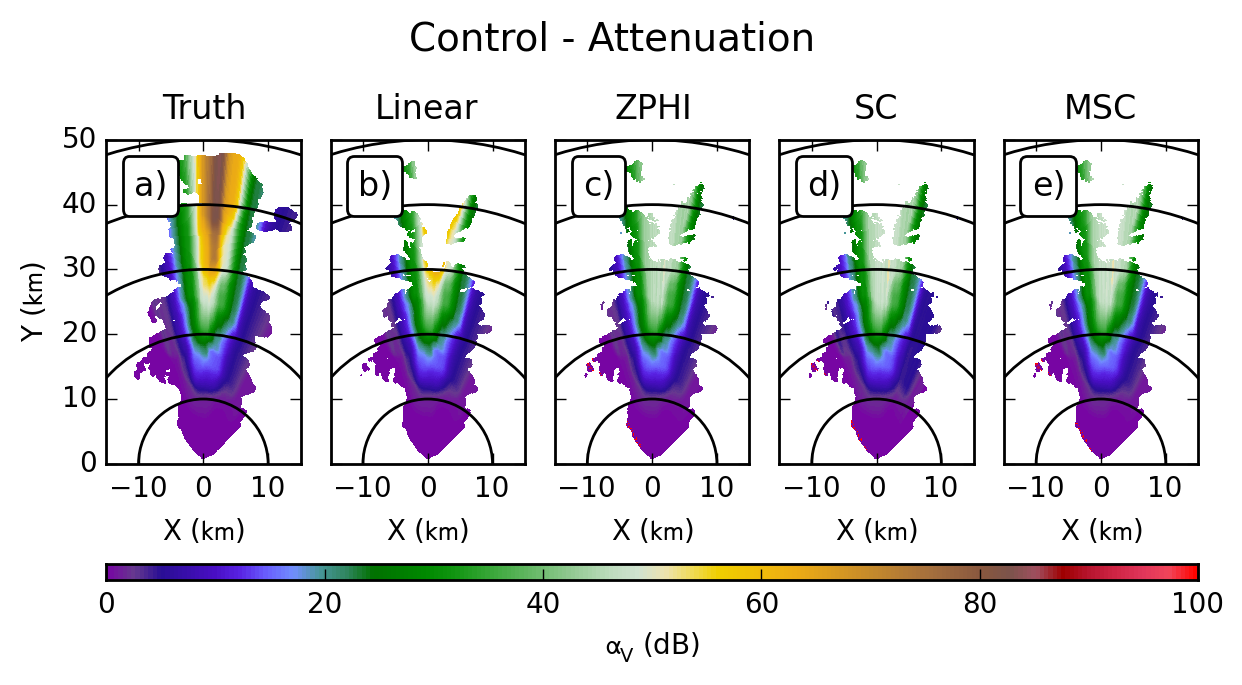
\includegraphics[scale=0.7]{figures/X_Control_Attenuation_V}
    \end{center}
\end{frame}

\begin{frame}
    \begin{center}
        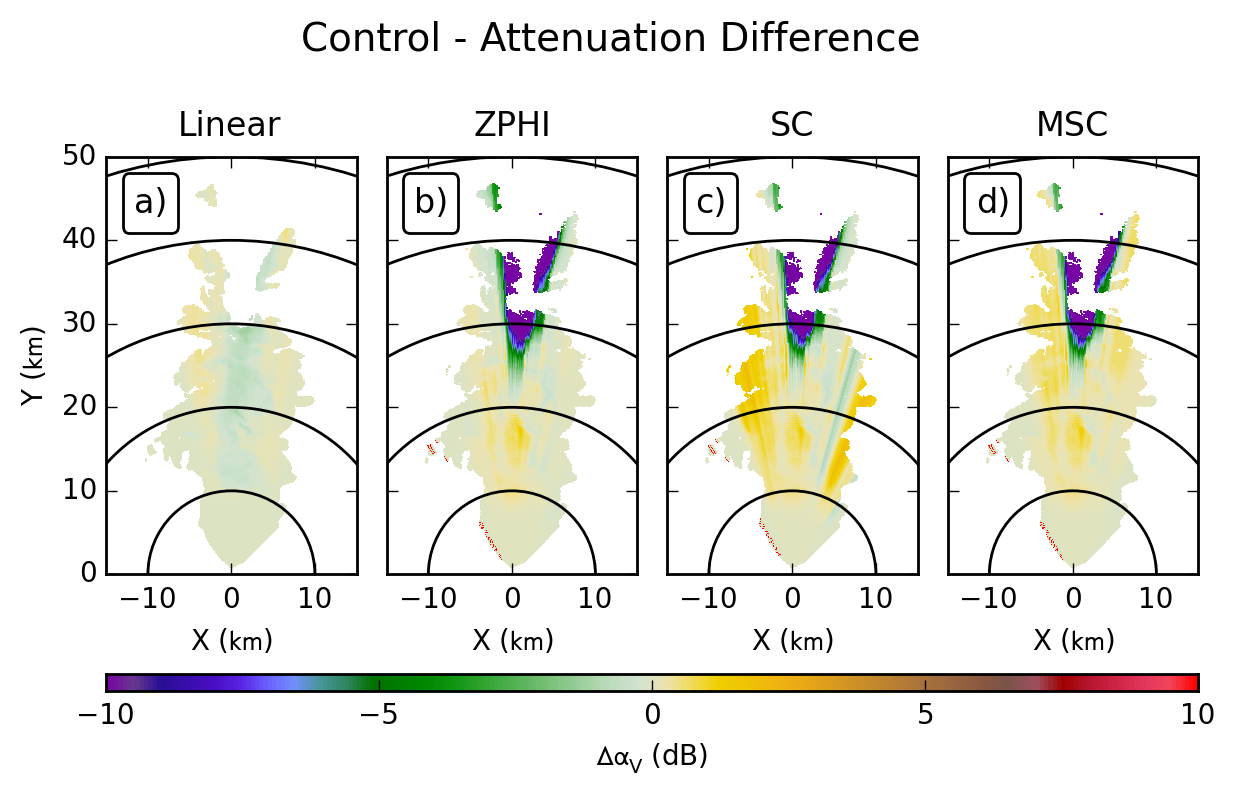
\includegraphics[scale=0.7]{figures/X_Control_Attenuation_Difference_V}
    \end{center}
\end{frame}

\begin{frame}
    \begin{center}
        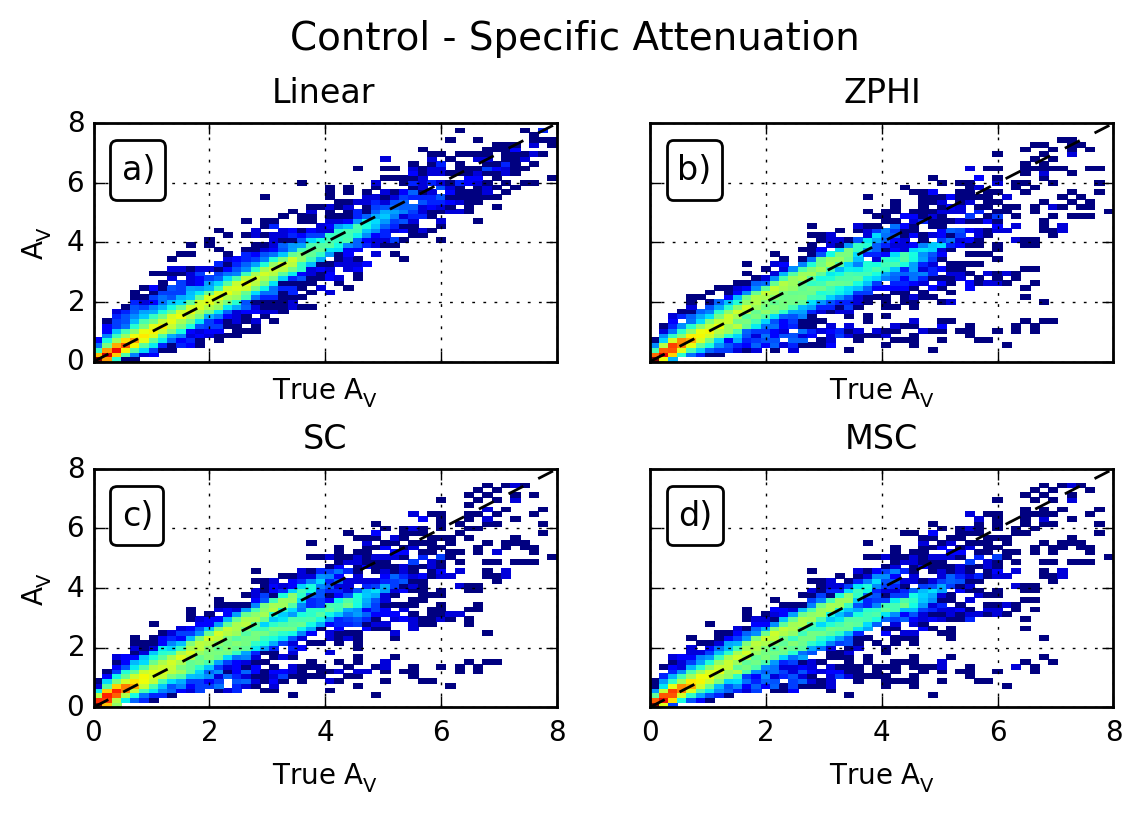
\includegraphics[scale=0.7]{figures/X_Control_Specific_Attenuation_V_scatter}
    \end{center}
\end{frame}

\begin{frame}
    \begin{center}
        \includegraphics<1>[scale=0.7]{figures/C_Canting_Attenuation_V}
        \includegraphics<2>[scale=0.7]{figures/C_Control_Attenuation_V}
    \end{center}
\end{frame}

\begin{frame}
    \begin{center}
        \includegraphics<1>[scale=0.7]{figures/C_Canting_Attenuation_Difference_V}
        \includegraphics<2>[scale=0.7]{figures/C_Control_Attenuation_Difference_V}
    \end{center}
\end{frame}

\begin{frame}
    \begin{center}
        \includegraphics<1>[scale=0.7]{figures/C_Canting_Specific_Attenuation_V_scatter}
        \includegraphics<2>[scale=0.7]{figures/C_Control_Specific_Attenuation_V_scatter}
    \end{center}
\end{frame}

\begin{frame}
    \begin{center}
        \includegraphics<1>[scale=0.7]{figures/X_Canting_Attenuation_V}
        \includegraphics<2>[scale=0.7]{figures/X_Control_Attenuation_V}
    \end{center}
\end{frame}

\begin{frame}
    \begin{center}
        \includegraphics<1>[scale=0.7]{figures/X_Canting_Attenuation_Difference_V}
        \includegraphics<2>[scale=0.7]{figures/X_Control_Attenuation_Difference_V}
    \end{center}
\end{frame}

\begin{frame}
    \begin{center}
        \includegraphics<1>[scale=0.7]{figures/X_Canting_Specific_Attenuation_V_scatter}
        \includegraphics<2>[scale=0.7]{figures/X_Control_Specific_Attenuation_V_scatter}
    \end{center}
\end{frame}

\begin{frame}
    \begin{center}
        \includegraphics<1>[scale=0.7]{figures/C_Shape_Attenuation_V}
        \includegraphics<2>[scale=0.7]{figures/C_Control_Attenuation_V}
    \end{center}
\end{frame}

\begin{frame}
    \begin{center}
        \includegraphics<1>[scale=0.7]{figures/C_Shape_Attenuation_Difference_V}
        \includegraphics<2>[scale=0.7]{figures/C_Control_Attenuation_Difference_V}
    \end{center}
\end{frame}

\begin{frame}
    \begin{center}
        \includegraphics<1>[scale=0.7]{figures/C_Shape_Specific_Attenuation_V_scatter}
        \includegraphics<2>[scale=0.7]{figures/C_Control_Specific_Attenuation_V_scatter}
    \end{center}
\end{frame}

\begin{frame}
    \begin{center}
        \includegraphics<1>[scale=0.7]{figures/X_Shape_Attenuation_V}
        \includegraphics<2>[scale=0.7]{figures/X_Control_Attenuation_V}
    \end{center}
\end{frame}

\begin{frame}
    \begin{center}
        \includegraphics<1>[scale=0.7]{figures/X_Shape_Attenuation_Difference_V}
        \includegraphics<2>[scale=0.7]{figures/X_Control_Attenuation_Difference_V}
    \end{center}
\end{frame}

\begin{frame}
    \begin{center}
        \includegraphics<1>[scale=0.7]{figures/X_Shape_Specific_Attenuation_V_scatter}
        \includegraphics<2>[scale=0.7]{figures/X_Control_Specific_Attenuation_V_scatter}
    \end{center}
\end{frame}

\begin{frame}
    \begin{center}
        \includegraphics<1>[scale=0.7]{figures/C_Temperature_Attenuation_V}
        \includegraphics<2>[scale=0.7]{figures/C_Control_Attenuation_V}
    \end{center}
\end{frame}

\begin{frame}
    \begin{center}
        \includegraphics<1>[scale=0.7]{figures/C_Temperature_Attenuation_Difference_V}
        \includegraphics<2>[scale=0.7]{figures/C_Control_Attenuation_Difference_V}
    \end{center}
\end{frame}

\begin{frame}
    \begin{center}
        \includegraphics<1>[scale=0.7]{figures/C_Temperature_Specific_Attenuation_V_scatter}
        \includegraphics<2>[scale=0.7]{figures/C_Control_Specific_Attenuation_V_scatter}
    \end{center}
\end{frame}

\begin{frame}
    \begin{center}
        \includegraphics<1>[scale=0.7]{figures/X_Temperature_Attenuation_V}
        \includegraphics<2>[scale=0.7]{figures/X_Control_Attenuation_V}
    \end{center}
\end{frame}

\begin{frame}
    \begin{center}
        \includegraphics<1>[scale=0.7]{figures/X_Temperature_Attenuation_Difference_V}
        \includegraphics<2>[scale=0.7]{figures/X_Control_Attenuation_Difference_V}
    \end{center}
\end{frame}

\begin{frame}
    \begin{center}
        \includegraphics<1>[scale=0.7]{figures/X_Temperature_Specific_Attenuation_V_scatter}
        \includegraphics<2>[scale=0.7]{figures/X_Control_Specific_Attenuation_V_scatter}
    \end{center}
\end{frame}

\begin{frame}
    \begin{center}
        \includegraphics<1>[scale=0.7]{figures/C_Wavelength_Attenuation_V}
        \includegraphics<2>[scale=0.7]{figures/C_Control_Attenuation_V}
    \end{center}
\end{frame}

\begin{frame}
    \begin{center}
        \includegraphics<1>[scale=0.7]{figures/C_Wavelength_Attenuation_Difference_V}
        \includegraphics<2>[scale=0.7]{figures/C_Control_Attenuation_Difference_V}
    \end{center}
\end{frame}

\begin{frame}
    \begin{center}
        \includegraphics<1>[scale=0.7]{figures/C_Wavelength_Specific_Attenuation_V_scatter}
        \includegraphics<2>[scale=0.7]{figures/C_Control_Specific_Attenuation_V_scatter}
    \end{center}
\end{frame}

\begin{frame}
    \begin{center}
        \includegraphics<1>[scale=0.7]{figures/X_Wavelength_Attenuation_V}
        \includegraphics<2>[scale=0.7]{figures/X_Control_Attenuation_V}
    \end{center}
\end{frame}

\begin{frame}
    \begin{center}
        \includegraphics<1>[scale=0.7]{figures/X_Wavelength_Attenuation_Difference_V}
        \includegraphics<2>[scale=0.7]{figures/X_Control_Attenuation_Difference_V}
    \end{center}
\end{frame}

\begin{frame}
    \begin{center}
        \includegraphics<1>[scale=0.7]{figures/X_Wavelength_Specific_Attenuation_V_scatter}
        \includegraphics<2>[scale=0.7]{figures/X_Control_Specific_Attenuation_V_scatter}
    \end{center}
\end{frame}

\begin{frame}
    \begin{center}
        \includegraphics<1>[scale=0.7]{figures/C_Combined_Attenuation_V}
        \includegraphics<2>[scale=0.7]{figures/C_Control_Attenuation_V}
    \end{center}
\end{frame}

\begin{frame}
    \begin{center}
        \includegraphics<1>[scale=0.7]{figures/C_Combined_Attenuation_Difference_V}
        \includegraphics<2>[scale=0.7]{figures/C_Control_Attenuation_Difference_V}
    \end{center}
\end{frame}

\begin{frame}
    \begin{center}
        \includegraphics<1>[scale=0.7]{figures/C_Combined_Specific_Attenuation_V_scatter}
        \includegraphics<2>[scale=0.7]{figures/C_Control_Specific_Attenuation_V_scatter}
    \end{center}
\end{frame}

\begin{frame}
    \begin{center}
        \includegraphics<1>[scale=0.7]{figures/X_Combined_Attenuation_V}
        \includegraphics<2>[scale=0.7]{figures/X_Control_Attenuation_V}
    \end{center}
\end{frame}

\begin{frame}
    \begin{center}
        \includegraphics<1>[scale=0.7]{figures/X_Combined_Attenuation_Difference_V}
        \includegraphics<2>[scale=0.7]{figures/X_Control_Attenuation_Difference_V}
    \end{center}
\end{frame}

\begin{frame}
    \begin{center}
        \includegraphics<1>[scale=0.7]{figures/X_Combined_Specific_Attenuation_V_scatter}
        \includegraphics<2>[scale=0.7]{figures/X_Control_Specific_Attenuation_V_scatter}
    \end{center}
\end{frame}

\begin{frame}
    \frametitle{Summary: MSE at C-band for Horizontal Polarization (\si{dB\squared\per \kilo\meter\squared})}
    \begin{center}
        \begin{tabular}{| c | c | c | c | c |}
            \hline
            Experiment & Linear & ZPHI & SC & MSC \\
            \hline
            \hline
            Control & 0.0047 & 0.0070 & 0.0070 & 0.0059 \\
            Canting & 0.0068 & 0.0094 & 0.0071 & 0.0060 \\
            Shape & 0.0251 & 0.0379 & 0.0079 & 0.0070 \\
            Temperature & 0.0191 & 0.0230 & 0.0062 & 0.0050 \\
            Wavelength & 0.0171 & 0.0259 & 0.0123 & 0.0117 \\
            Combined & 0.0302 & 0.0478 & 0.0132 & 0.0143 \\
            \hline
        \end{tabular}
    \end{center}
\end{frame}

\begin{frame}
    \frametitle{Summary: $r^2$ at C-band for Horizontal Polarization}
    \begin{center}
        \begin{tabular}{| c | c | c | c | c |}
            \hline
            Experiment & Linear & ZPHI & SC & MSC \\
            \hline
            \hline
            Control & 0.9612 & 0.9233 & 0.9173 & 0.9305 \\
            Canting & 0.9612 & 0.9136 & 0.9165 & 0.9306 \\
            Shape & 0.9560 & 0.8265 & 0.9083 & 0.9279 \\
            Temperature & 0.9554 & 0.8453 & 0.8974 & 0.9235 \\
            Wavelength & 0.9596 & 0.9002 & 0.9304 & 0.9351 \\
            Combined & 0.9418 & 0.8375 & 0.9128 & 0.9202 \\
            \hline
        \end{tabular}
    \end{center}
\end{frame}

\begin{frame}
    \frametitle{Summary: Bias at C-band for Vertical Polarization (\si{dB\per \kilo\meter})}
    \begin{center}
        \begin{tabular}{| c | c | c | c | c |}
            \hline
            Experiment & Linear & ZPHI & SC & MSC \\
            \hline
            \hline
            Control & 0.0095 & 0.0071 & -0.0027 & -0.0087 \\
            Canting & 0.0243 & 0.0214 & -0.0024 & -0.0096 \\
            Shape & 0.0819 & 0.0803 & 0.0070 & -0.0074 \\
            Temperature & 0.0727 & 0.0689 & -0.0022 & -0.0135 \\
            Wavelength & -0.0704 & -0.0701 & -0.0020 & -0.0063 \\
            Combined & 0.1050 & 0.1027 & 0.0107 & -0.0093 \\
            \hline
        \end{tabular}
    \end{center}
\end{frame}

\begin{frame}
    \frametitle{Summary: MSE at C-band for Vertical Polarization (\si{dB\squared\per \kilo\meter\squared})}
    \begin{center}
        \begin{tabular}{| c | c | c | c | c |}
            \hline
            Experiment & Linear & ZPHI & SC & MSC \\
            \hline
            \hline
            Control & 0.0020 & 0.0033 & 0.0042 & 0.0034 \\
            Canting & 0.0032 & 0.0041 & 0.0042 & 0.0034 \\
            Shape & 0.0128 & 0.0167 & 0.0040 & 0.0034 \\
            Temperature & 0.0111 & 0.0112 & 0.0036 & 0.0028 \\
            Wavelength & 0.0125 & 0.0191 & 0.0074 & 0.0069 \\
            Combined & 0.0187 & 0.0259 & 0.0063 & 0.0065 \\
            \hline
        \end{tabular}
    \end{center}
\end{frame}

\begin{frame}
    \frametitle{Summary: $r^2$ at C-band for Vertical Polarization}
    \begin{center}
        \begin{tabular}{| c | c | c | c | c |}
            \hline
            Experiment & Linear & ZPHI & SC & MSC \\
            \hline
            \hline
            Control & 0.9639 & 0.9240 & 0.9061 & 0.9257 \\
            Canting & 0.9642 & 0.9173 & 0.9037 & 0.9254 \\
            Shape & 0.9621 & 0.8616 & 0.9055 & 0.9273 \\
            Temperature & 0.9617 & 0.8652 & 0.8695 & 0.9175 \\
            Wavelength & 0.9627 & 0.8922 & 0.9244 & 0.9318 \\
            Combined & 0.9512 & 0.8402 & 0.9085 & 0.9221 \\
            \hline
        \end{tabular}
    \end{center}
\end{frame}

\begin{frame}
    \frametitle{Summary: MSE at C-band for Differential Polarization (\si{dB\squared\per \kilo\meter\squared})}
    \begin{center}
        \begin{tabular}{| c | c | c | c | c |}
            \hline
            Experiment & Linear & ZPHI & SC & MSC \\
            \hline
            \hline
            Control & 0.0023 & 0.0019 & 0.0012 & 0.0009 \\
            Canting & 0.0026 & 0.0024 & 0.0013 & 0.0010 \\
            Shape & 0.0056 & 0.0082 & 0.0012 & 0.0014 \\
            Temperature & 0.0037 & 0.0043 & 0.0013 & 0.0010 \\
            Wavelength & 0.0015 & 0.0019 & 0.0018 & 0.0014 \\
            Combined & 0.0044 & 0.0063 & 0.0025 & 0.0029 \\
            \hline
        \end{tabular}
    \end{center}
\end{frame}

\begin{frame}
    \frametitle{Summary: $r^2$ at C-band for Differential Polarization}
    \begin{center}
        \begin{tabular}{| c | c | c | c | c |}
            \hline
            Experiment & Linear & ZPHI & SC & MSC \\
            \hline
            \hline
            Control & 0.9021 & 0.8291 & 0.8315 & 0.8896 \\
            Canting & 0.9035 & 0.8030 & 0.8336 & 0.8916 \\
            Shape & 0.8986 & 0.5224 & 0.8437 & 0.8586 \\
            Temperature & 0.8869 & 0.6153 & 0.8099 & 0.8850 \\
            Wavelength & 0.9129 & 0.8474 & 0.8652 & 0.8895 \\
            Combined & 0.8924 & 0.7293 & 0.8605 & 0.8465 \\
            \hline
        \end{tabular}
    \end{center}
\end{frame}

\begin{frame}
    \frametitle{Summary: MSE at X-band for Horizontal Polarization (\si{dB\squared\per \kilo\meter\squared})}
    \begin{center}
        \begin{tabular}{| c | c | c | c | c |}
            \hline
            Experiment & Linear & ZPHI & SC & MSC \\
            \hline
            \hline
            Control & 0.0722 & 0.2279 & 0.2200 & 0.1985 \\
            Canting & 0.0862 & 0.1882 & 0.2225 & 0.1977 \\
            Shape & 0.4232 & 0.9875 & 0.2623 & 0.2282 \\
            Temperature & 0.1073 & 0.3614 & 0.2654 & 0.2546 \\
            Wavelength & 0.1323 & 0.5343 & 0.2619 & 0.2398 \\
            Combined & 0.2691 & 0.4268 & 0.4510 & 0.4748 \\
            \hline
        \end{tabular}
    \end{center}
\end{frame}

\begin{frame}
    \frametitle{Summary: $r^2$ at X-band for Horizontal Polarization}
    \begin{center}
        \begin{tabular}{| c | c | c | c | c |}
            \hline
            Experiment & Linear & ZPHI & SC & MSC \\
            \hline
            \hline
            Control & 0.9708 & 0.9058 & 0.9082 & 0.9157 \\
            Canting & 0.9709 & 0.9200 & 0.9080 & 0.9167 \\
            Shape & 0.9667 & 0.7668 & 0.8933 & 0.9066 \\
            Temperature & 0.9682 & 0.8760 & 0.9053 & 0.9081 \\
            Wavelength & 0.9726 & 0.8485 & 0.9178 & 0.9233 \\
            Combined & 0.9653 & 0.8988 & 0.8867 & 0.8811 \\
            \hline
        \end{tabular}
    \end{center}
\end{frame}

\begin{frame}
    \frametitle{Summary: Bias at X-band for Vertical Polarization (\si{dB\per \kilo\meter})}
    \begin{center}
        \begin{tabular}{| c | c | c | c | c |}
            \hline
            Experiment & Linear & ZPHI & SC & MSC \\
            \hline
            \hline
            Control & -0.0004 & -0.0414 & 0.0036 & -0.0115 \\
            Canting & 0.0716 & 0.0250 & 0.0066 & -0.0102 \\
            Shape & 0.4093 & 0.3619 & 0.0232 & 0.0090 \\
            Temperature & -0.0363 & -0.0767 & 0.0064 & -0.0043 \\
            Wavelength & -0.1521 & -0.1931 & -0.0081 & -0.0267 \\
            Combined & 0.3115 & 0.2453 & 0.0033 & -0.0330 \\
            \hline
        \end{tabular}
    \end{center}
\end{frame}

\begin{frame}
    \frametitle{Summary: MSE at X-band for Vertical Polarization (\si{dB\squared\per \kilo\meter\squared})}
    \begin{center}
        \begin{tabular}{| c | c | c | c | c |}
            \hline
            Experiment & Linear & ZPHI & SC & MSC \\
            \hline
            \hline
            Control & 0.0500 & 0.1607 & 0.1533 & 0.1418 \\
            Canting & 0.0597 & 0.1284 & 0.1530 & 0.1392 \\
            Shape & 0.3313 & 0.9809 & 0.1687 & 0.1530 \\
            Temperature & 0.0770 & 0.2473 & 0.1798 & 0.1772 \\
            Wavelength & 0.1064 & 0.4143 & 0.1994 & 0.1900 \\
            Combined & 0.2088 & 0.3956 & 0.2802 & 0.3185 \\
            \hline
        \end{tabular}
    \end{center}
\end{frame}

\begin{frame}
    \frametitle{Summary: $r^2$ at X-band for Vertical Polarization}
    \begin{center}
        \begin{tabular}{| c | c | c | c | c |}
            \hline
            Experiment & Linear & ZPHI & SC & MSC \\
            \hline
            \hline
            Control & 0.9712 & 0.9071 & 0.9098 & 0.9160 \\
            Canting & 0.9713 & 0.9219 & 0.9091 & 0.9166 \\
            Shape & 0.9678 & 0.7046 & 0.8981 & 0.9078 \\
            Temperature & 0.9687 & 0.8821 & 0.9101 & 0.9114 \\
            Wavelength & 0.9727 & 0.8389 & 0.9123 & 0.9161 \\
            Combined & 0.9659 & 0.8777 & 0.8933 & 0.8815 \\
            \hline
        \end{tabular}
    \end{center}
\end{frame}

\begin{frame}
    \frametitle{Summary: MSE at X-band for Differential Polarization (\si{dB\squared\per \kilo\meter\squared})}
    \begin{center}
        \begin{tabular}{| c | c | c | c | c |}
            \hline
            Experiment & Linear & ZPHI & SC & MSC \\
            \hline
            \hline
            Control & 0.0044 & 0.0120 & 0.0118 & 0.0117 \\
            Canting & 0.0049 & 0.0120 & 0.0129 & 0.0129 \\
            Shape & 0.0116 & 0.3639 & 0.0172 & 0.0169 \\
            Temperature & 0.0039 & 0.0166 & 0.0148 & 0.0151 \\
            Wavelength & 0.0040 & 0.0211 & 0.0167 & 0.0163 \\
            Combined & 0.0082 & 0.0287 & 0.0298 & 0.0296 \\
            \hline
        \end{tabular}
    \end{center}
\end{frame}

\begin{frame}
    \frametitle{Summary: $r^2$ at X-band for Differential Polarization}
    \begin{center}
        \begin{tabular}{| c | c | c | c | c |}
            \hline
            Experiment & Linear & ZPHI & SC & MSC \\
            \hline
            \hline
            Control & 0.9561 & 0.8136 & 0.8197 & 0.8201 \\
            Canting & 0.9564 & 0.8322 & 0.8219 & 0.8216 \\
            Shape & 0.9537 & 0.3179 & 0.7968 & 0.8008 \\
            Temperature & 0.9565 & 0.7636 & 0.7909 & 0.7834 \\
            Wavelength & 0.9585 & 0.7163 & 0.7992 & 0.7970 \\
            Combined & 0.9565 & 0.7810 & 0.7549 & 0.7458 \\
            \hline
        \end{tabular}
    \end{center}
\end{frame}

\subsection{Spatial Errors}
\subsubsection{Control}
\begin{frame}
	\frametitle{Control: Standard Sampling}
	\begin{center}
	    \begin{tabular}{ | l | l | }
	        \hline
	        Radial Spacing & \SI{1.0}{\degree} \\
	        \SI{3}{dB} Beamwidth & \SI{1.0}{\degree} \\
	        Gate Width & \SI{125}{\meter} \\
			\hline
	    \end{tabular}
	\end{center}	
\end{frame}

\begin{frame}
    \begin{center}
        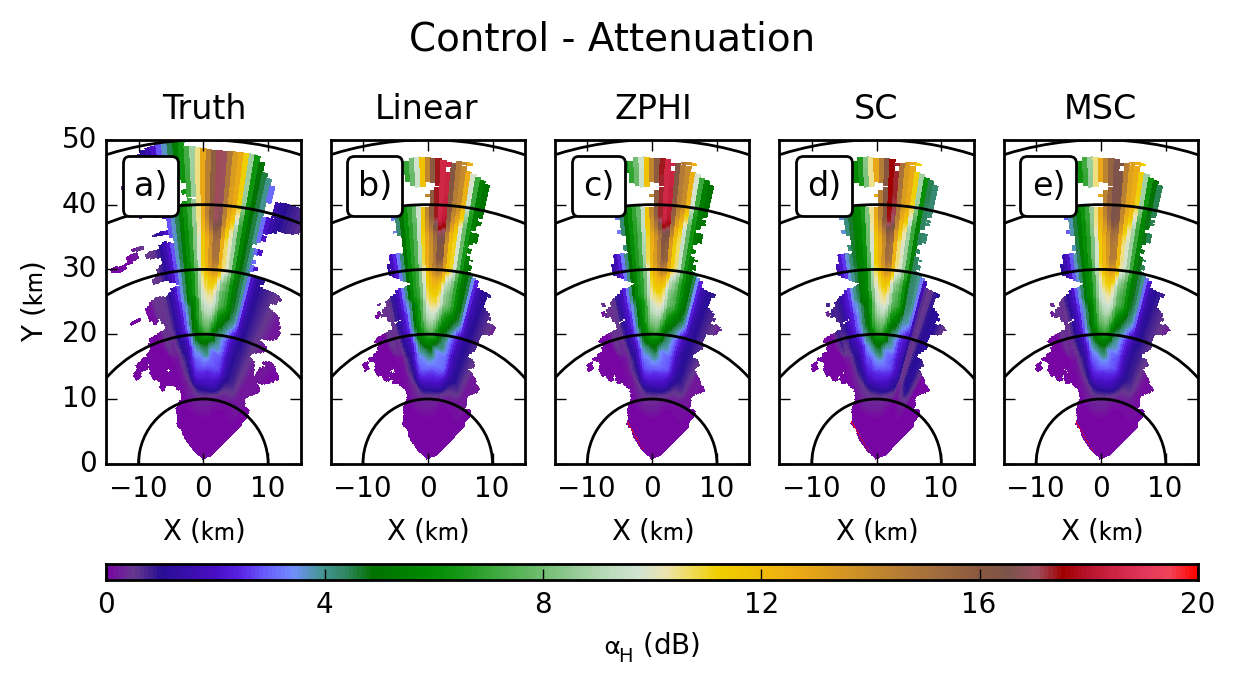
\includegraphics[scale=0.7]{figures/spatial/C_Control_Attenuation_H}
    \end{center}
\end{frame}

\begin{frame}
    \begin{center}
        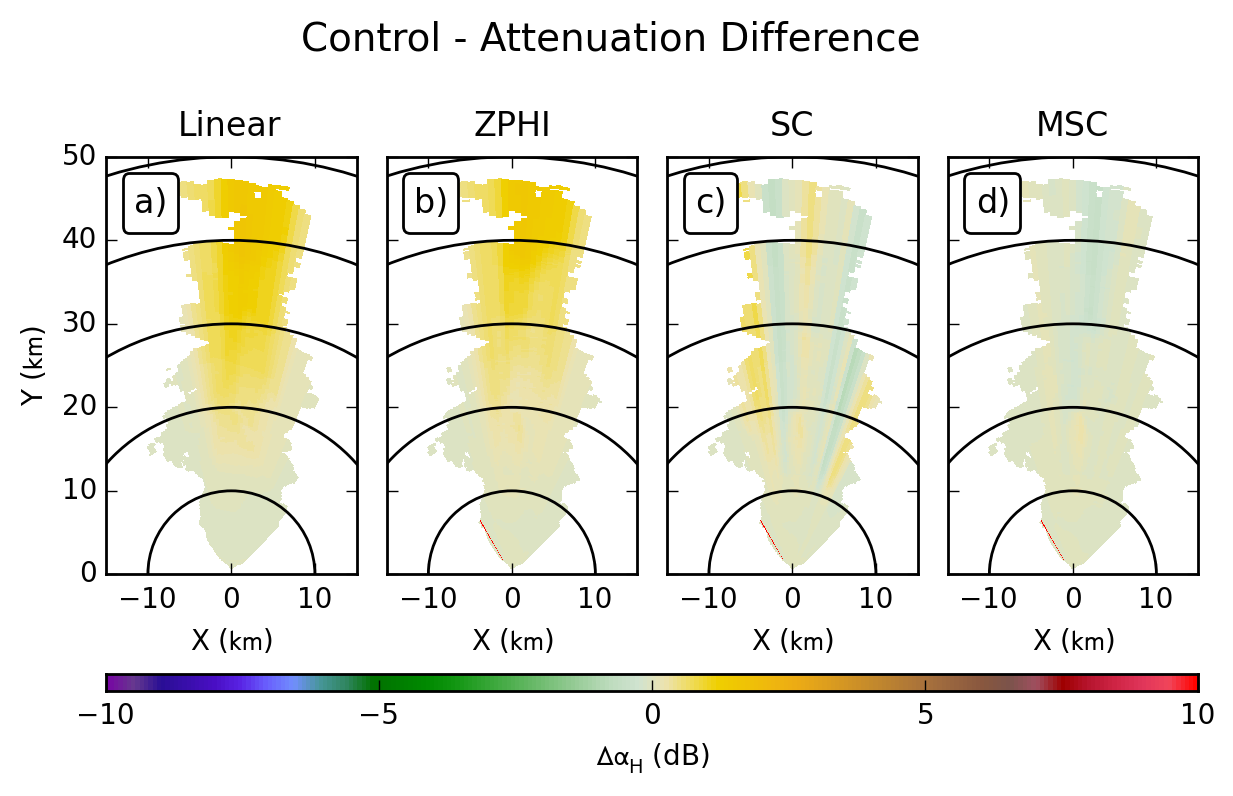
\includegraphics[scale=0.7]{figures/spatial/C_Control_Attenuation_Difference_H}
    \end{center}
\end{frame}

\begin{frame}
    \begin{center}
        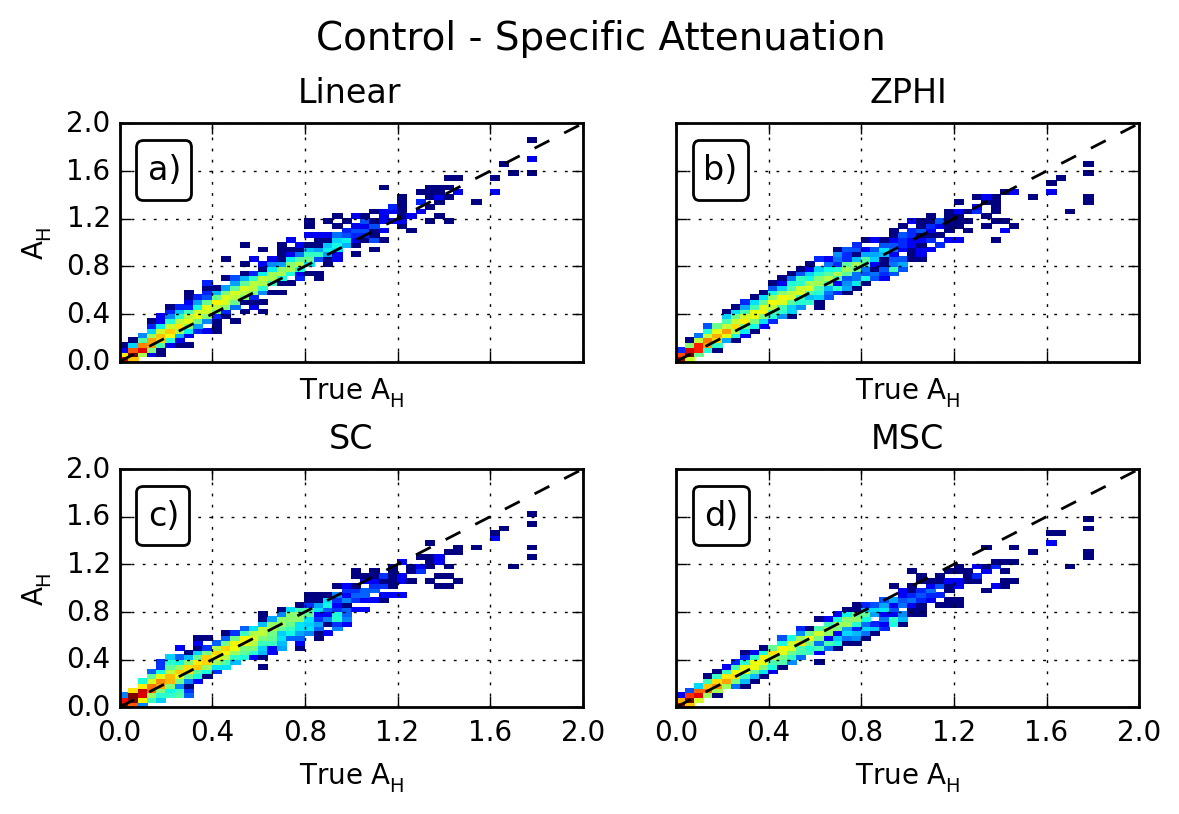
\includegraphics[scale=0.7]{figures/spatial/C_Control_Specific_Attenuation_H_scatter}
    \end{center}
\end{frame}

\begin{frame}
    \begin{center}
        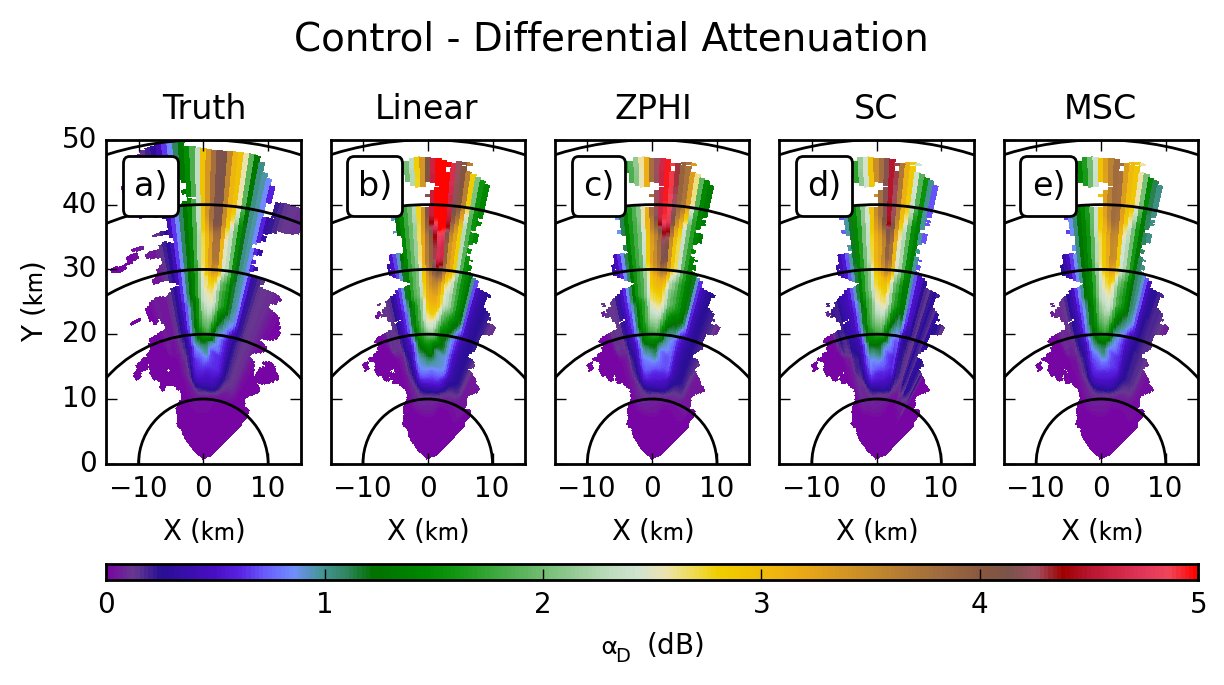
\includegraphics[scale=0.7]{figures/spatial/C_Control_Differential_Attenuation}
    \end{center}
\end{frame}

\begin{frame}
    \begin{center}
        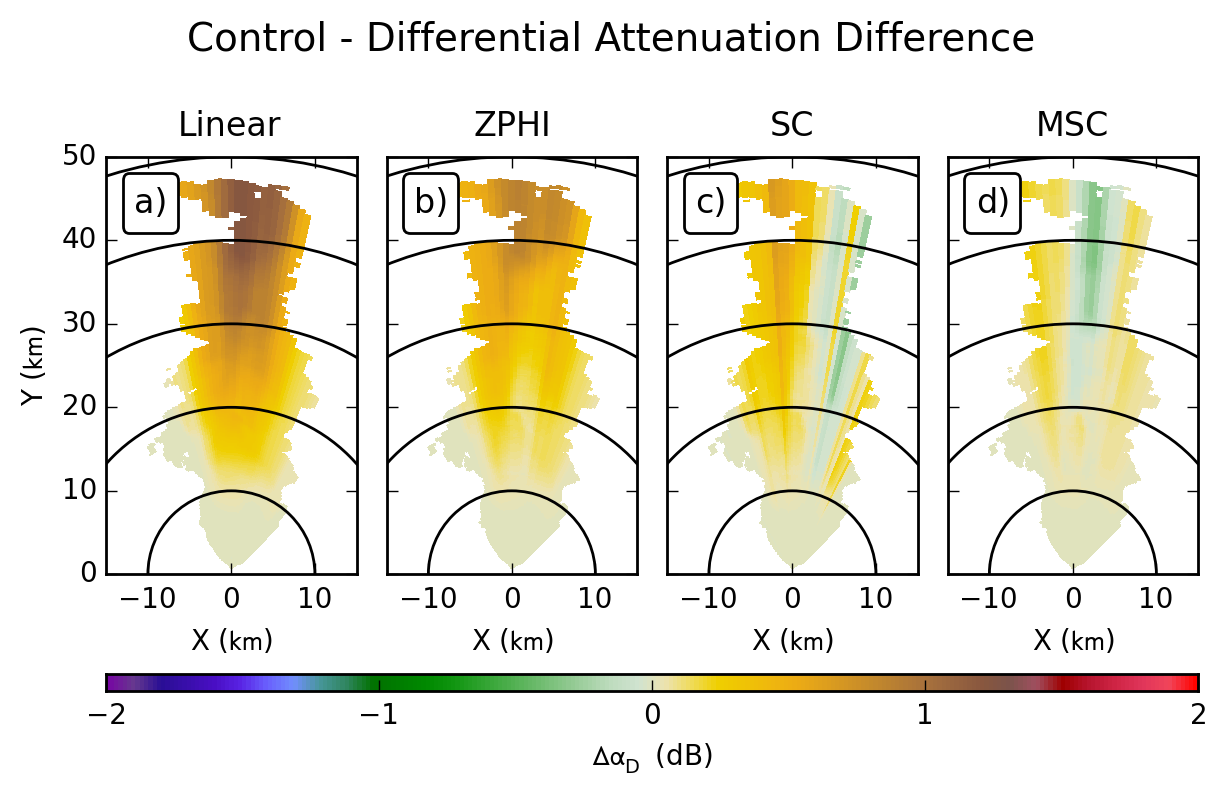
\includegraphics[scale=0.7]{figures/spatial/C_Control_Differential_Attenuation_Difference}
    \end{center}
\end{frame}

\begin{frame}
    \begin{center}
        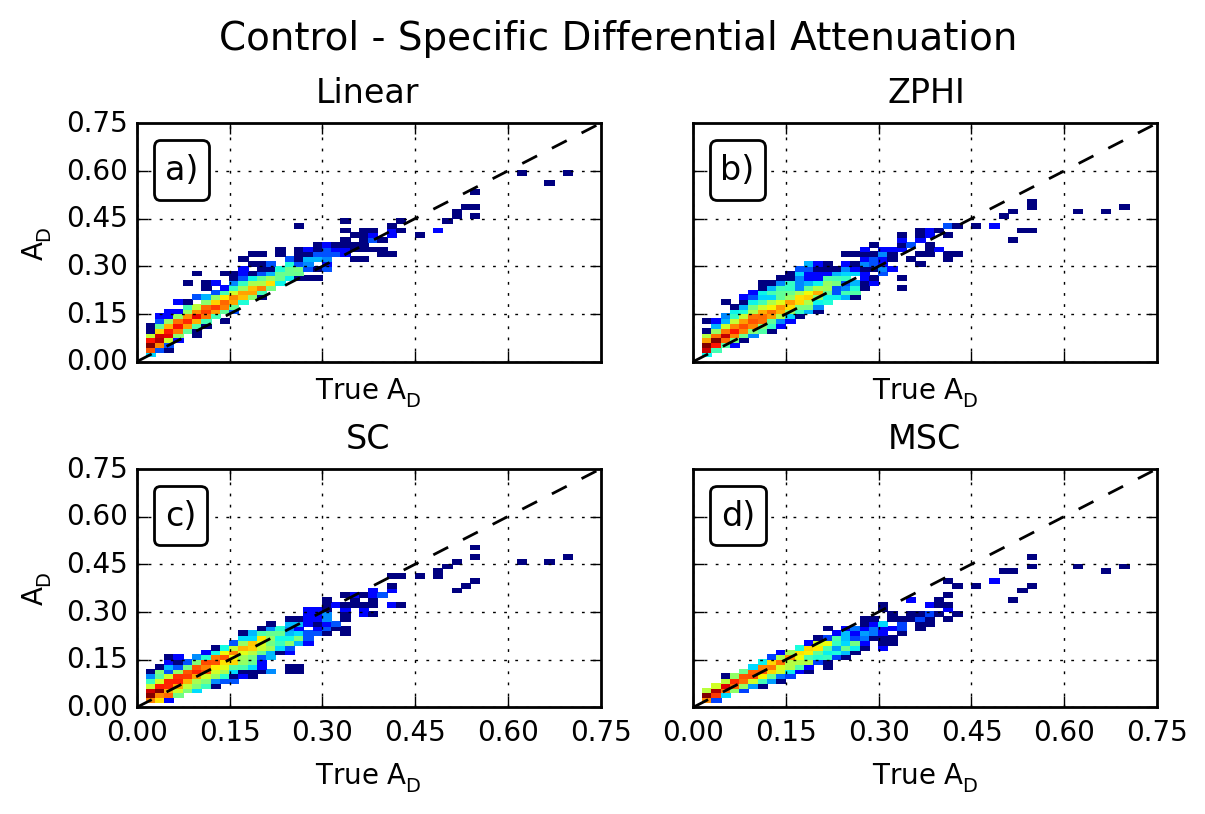
\includegraphics[scale=0.7]{figures/spatial/C_Control_Specific_Differential_Attenuation_scatter}
    \end{center}
\end{frame}

\begin{frame}
    \begin{center}
        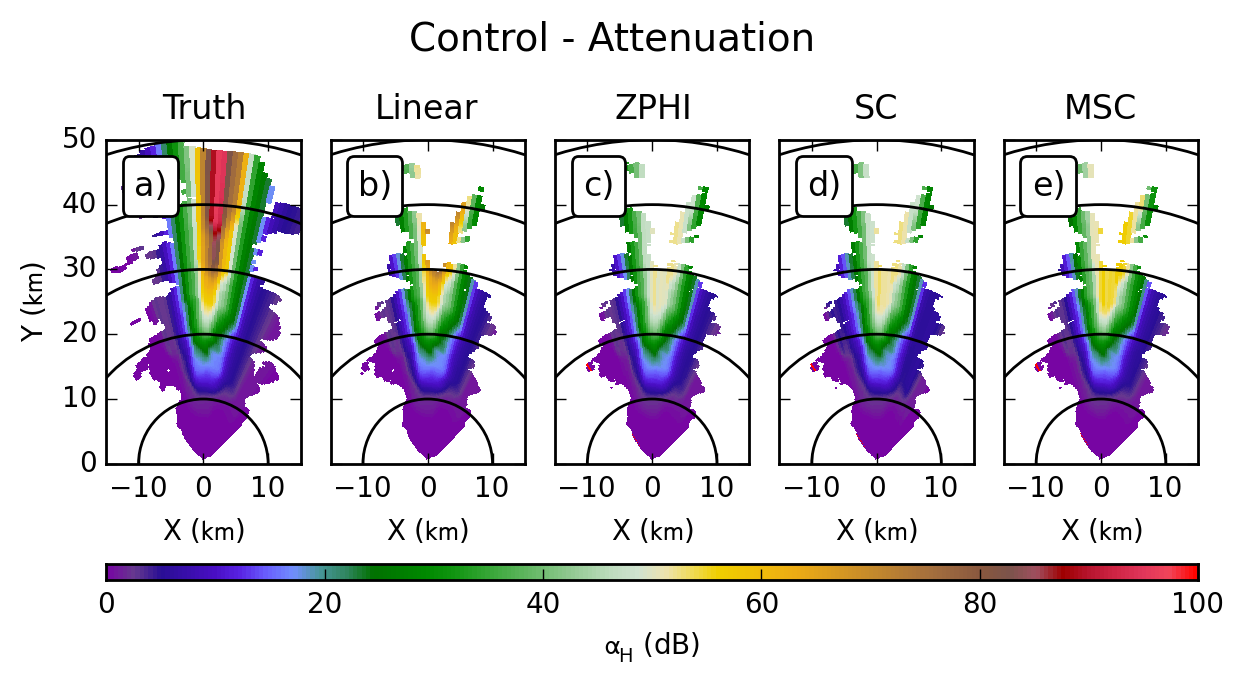
\includegraphics[scale=0.7]{figures/spatial/X_Control_Attenuation_H}
    \end{center}
\end{frame}

\begin{frame}
    \begin{center}
        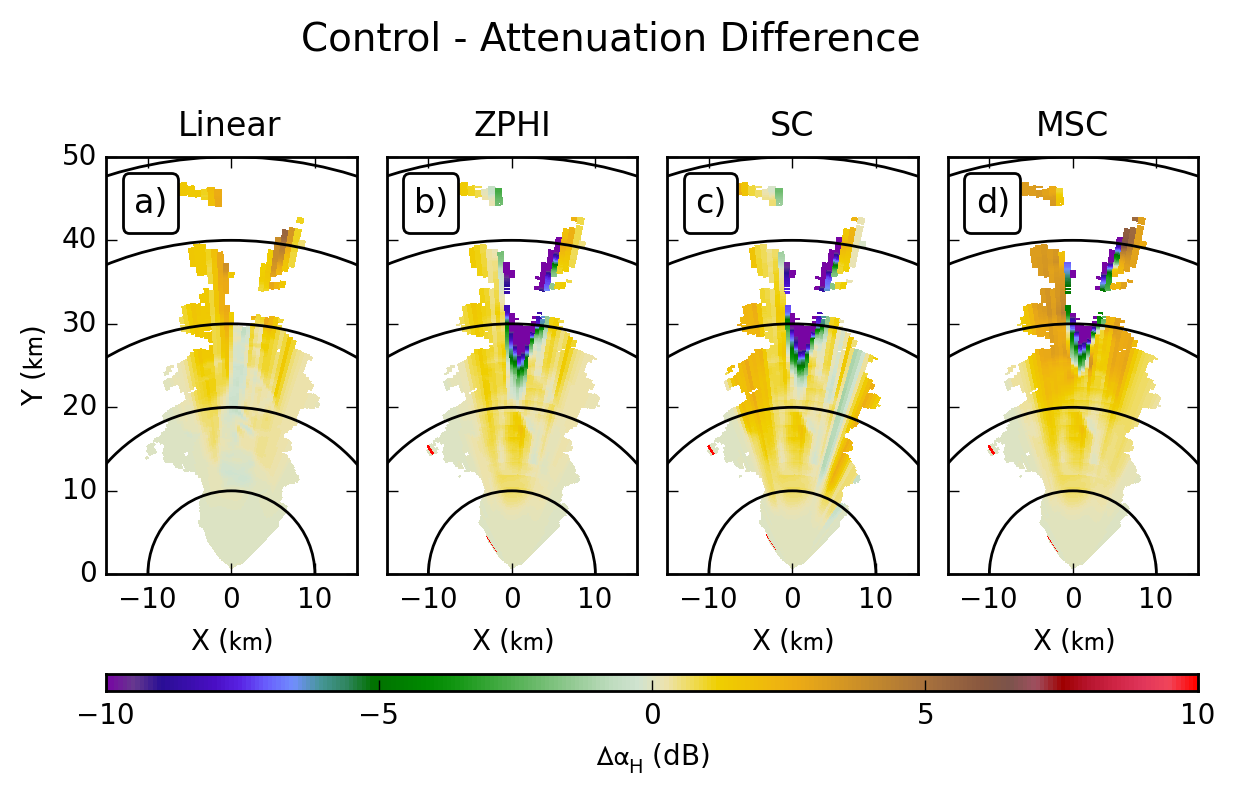
\includegraphics[scale=0.7]{figures/spatial/X_Control_Attenuation_Difference_H}
    \end{center}
\end{frame}

\begin{frame}
    \begin{center}
        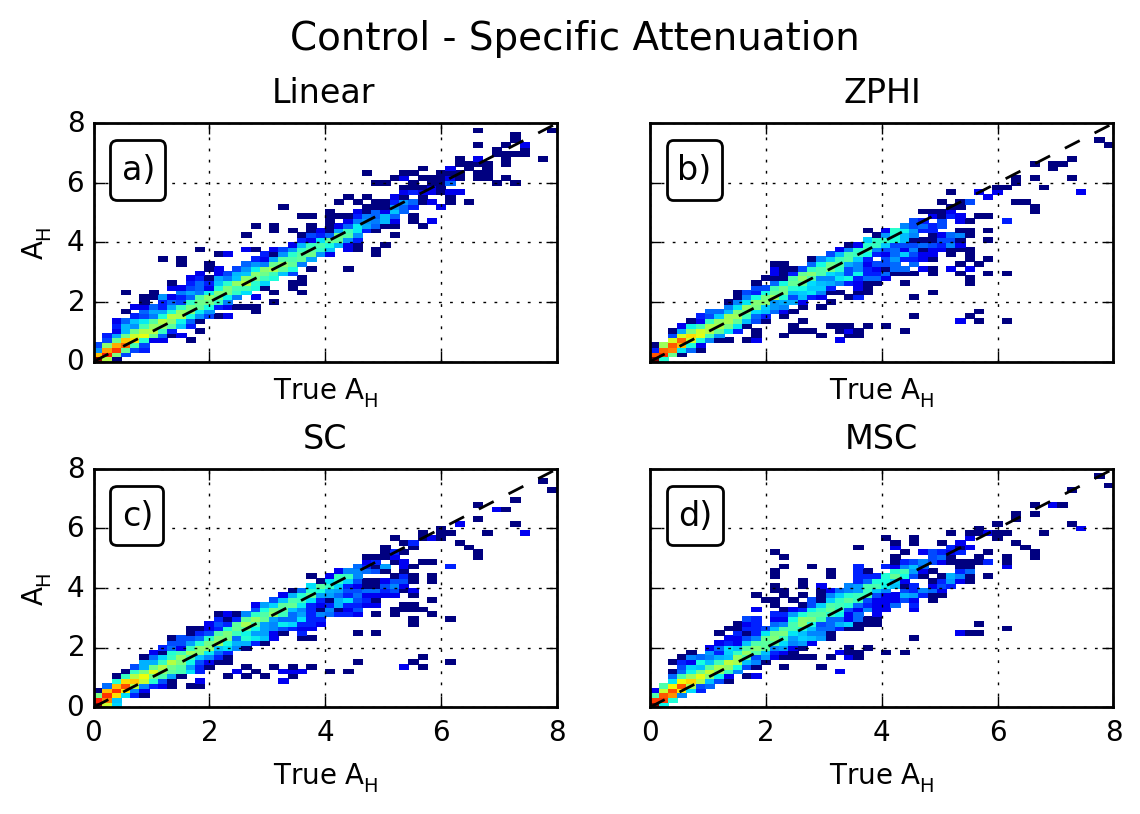
\includegraphics[scale=0.7]{figures/spatial/X_Control_Specific_Attenuation_H_scatter}
    \end{center}
\end{frame}

\begin{frame}
    \begin{center}
        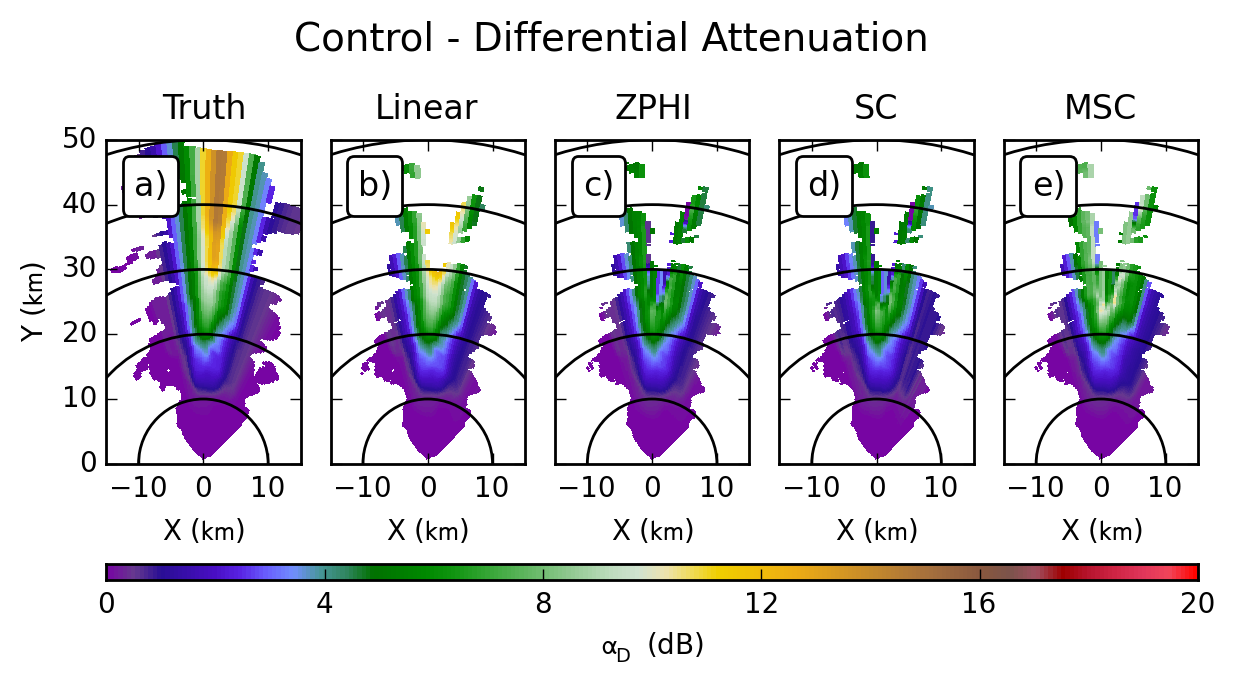
\includegraphics[scale=0.7]{figures/spatial/X_Control_Differential_Attenuation}
    \end{center}
\end{frame}

\begin{frame}
    \begin{center}
        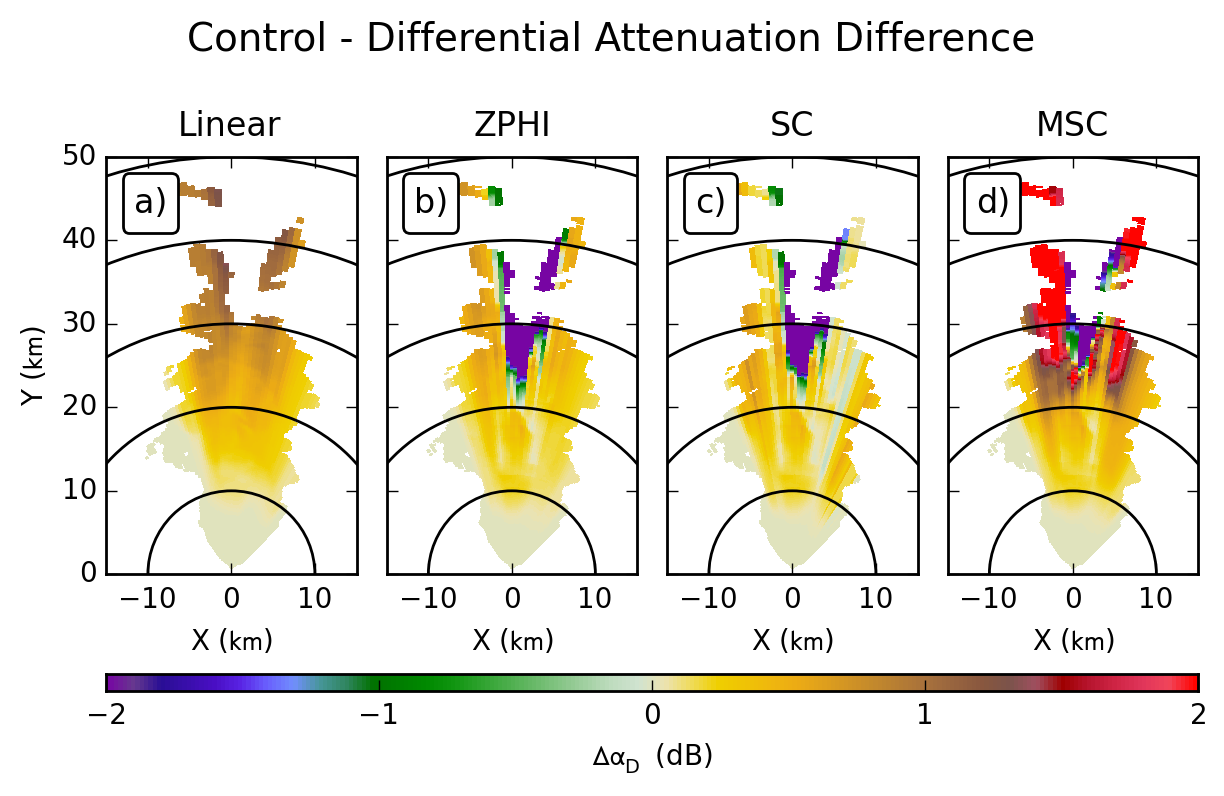
\includegraphics[scale=0.7]{figures/spatial/X_Control_Differential_Attenuation_Difference}
    \end{center}
\end{frame}

\begin{frame}
    \begin{center}
        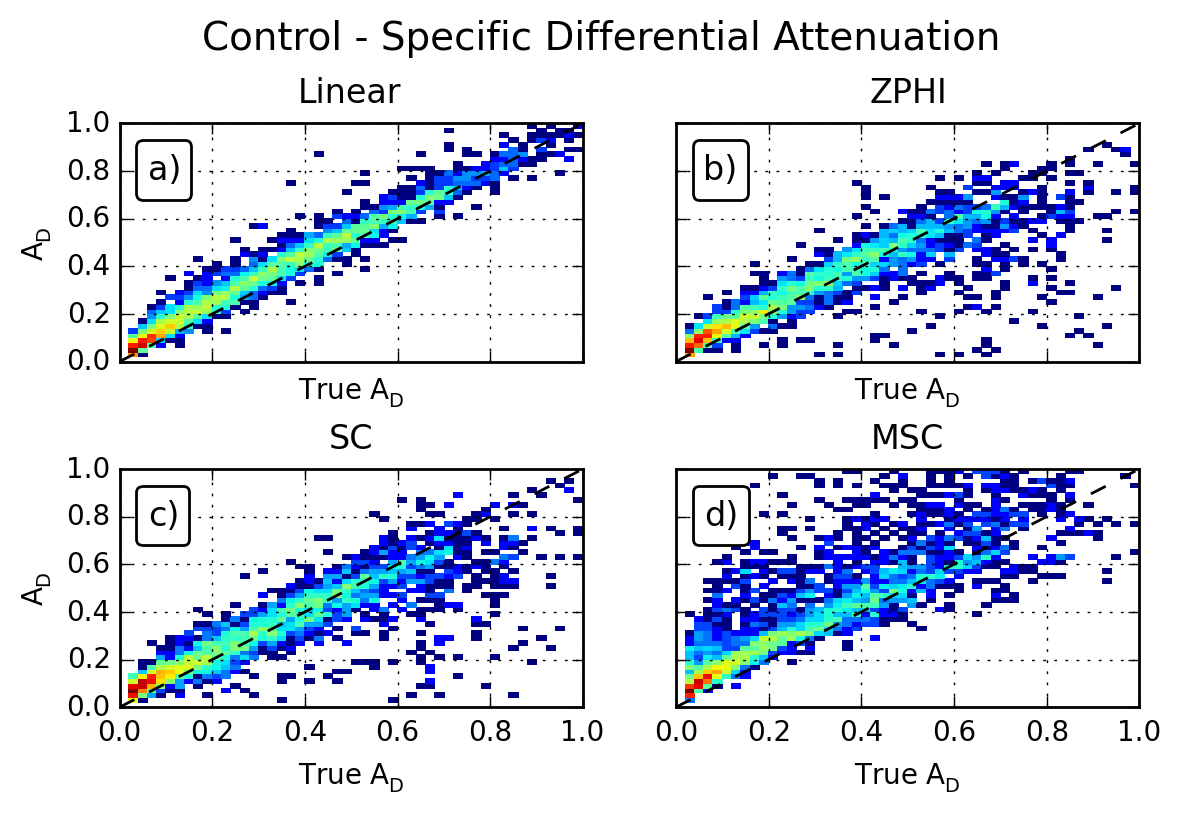
\includegraphics[scale=0.7]{figures/spatial/X_Control_Specific_Differential_Attenuation_scatter}
    \end{center}
\end{frame}

\subsubsection{Sidelobe}
\begin{frame}
    \begin{center}
        \includegraphics<1>[scale=0.7]{figures/spatial/C_Sidelobe_Attenuation_H}
        \includegraphics<2>[scale=0.7]{figures/spatial/C_Control_Attenuation_H}
    \end{center}
\end{frame}

\begin{frame}
    \begin{center}
        \includegraphics<1>[scale=0.7]{figures/spatial/C_Sidelobe_Attenuation_Difference_H}
        \includegraphics<2>[scale=0.7]{figures/spatial/C_Control_Attenuation_Difference_H}
    \end{center}
\end{frame}

\begin{frame}
    \begin{center}
        \includegraphics<1>[scale=0.7]{figures/spatial/C_Sidelobe_Specific_Attenuation_H_scatter}
        \includegraphics<2>[scale=0.7]{figures/spatial/C_Control_Specific_Attenuation_H_scatter}
    \end{center}
\end{frame}

\begin{frame}
    \begin{center}
        \includegraphics<1>[scale=0.7]{figures/spatial/C_Sidelobe_Differential_Attenuation}
        \includegraphics<2>[scale=0.7]{figures/spatial/C_Control_Differential_Attenuation}
    \end{center}
\end{frame}

\begin{frame}
    \begin{center}
        \includegraphics<1>[scale=0.7]{figures/spatial/C_Sidelobe_Differential_Attenuation_Difference}
        \includegraphics<2>[scale=0.7]{figures/spatial/C_Control_Differential_Attenuation_Difference}
    \end{center}
\end{frame}

\begin{frame}
    \begin{center}
        \includegraphics<1>[scale=0.7]{figures/spatial/C_Sidelobe_Specific_Differential_Attenuation_scatter}
        \includegraphics<2>[scale=0.7]{figures/spatial/C_Control_Specific_Differential_Attenuation_scatter}
    \end{center}
\end{frame}

\begin{frame}
    \begin{center}
        \includegraphics<1>[scale=0.7]{figures/spatial/X_Sidelobe_Attenuation_H}
        \includegraphics<2>[scale=0.7]{figures/spatial/X_Control_Attenuation_H}
    \end{center}
\end{frame}

\begin{frame}
    \begin{center}
        \includegraphics<1>[scale=0.7]{figures/spatial/X_Sidelobe_Attenuation_Difference_H}
        \includegraphics<2>[scale=0.7]{figures/spatial/X_Control_Attenuation_Difference_H}
    \end{center}
\end{frame}

\begin{frame}
    \begin{center}
        \includegraphics<1>[scale=0.7]{figures/spatial/X_Sidelobe_Specific_Attenuation_H_scatter}
        \includegraphics<2>[scale=0.7]{figures/spatial/X_Control_Specific_Attenuation_H_scatter}
    \end{center}
\end{frame}

\begin{frame}
    \begin{center}
        \includegraphics<1>[scale=0.7]{figures/spatial/X_Sidelobe_Differential_Attenuation}
        \includegraphics<2>[scale=0.7]{figures/spatial/X_Control_Differential_Attenuation}
    \end{center}
\end{frame}

\begin{frame}
    \begin{center}
        \includegraphics<1>[scale=0.7]{figures/spatial/X_Sidelobe_Differential_Attenuation_Difference}
        \includegraphics<2>[scale=0.7]{figures/spatial/X_Control_Differential_Attenuation_Difference}
    \end{center}
\end{frame}

\begin{frame}
    \begin{center}
        \includegraphics<1>[scale=0.7]{figures/spatial/X_Sidelobe_Specific_Differential_Attenuation_scatter}
        \includegraphics<2>[scale=0.7]{figures/spatial/X_Control_Specific_Differential_Attenuation_scatter}
    \end{center}
\end{frame}

\subsubsection{Beamwidth}
\begin{frame}
    \begin{center}
        \includegraphics<1>[scale=0.7]{figures/spatial/C_Beamwidth_Attenuation_H}
        \includegraphics<2>[scale=0.7]{figures/spatial/C_Control_Attenuation_H}
    \end{center}
\end{frame}

\begin{frame}
    \begin{center}
        \includegraphics<1>[scale=0.7]{figures/spatial/C_Beamwidth_Attenuation_Difference_H}
        \includegraphics<2>[scale=0.7]{figures/spatial/C_Control_Attenuation_Difference_H}
    \end{center}
\end{frame}

\begin{frame}
    \begin{center}
        \includegraphics<1>[scale=0.7]{figures/spatial/C_Beamwidth_Specific_Attenuation_H_scatter}
        \includegraphics<2>[scale=0.7]{figures/spatial/C_Control_Specific_Attenuation_H_scatter}
    \end{center}
\end{frame}

\begin{frame}
    \begin{center}
        \includegraphics<1>[scale=0.7]{figures/spatial/C_Beamwidth_Differential_Attenuation}
        \includegraphics<2>[scale=0.7]{figures/spatial/C_Control_Differential_Attenuation}
    \end{center}
\end{frame}

\begin{frame}
    \begin{center}
        \includegraphics<1>[scale=0.7]{figures/spatial/C_Beamwidth_Differential_Attenuation_Difference}
        \includegraphics<2>[scale=0.7]{figures/spatial/C_Control_Differential_Attenuation_Difference}
    \end{center}
\end{frame}

\begin{frame}
    \begin{center}
        \includegraphics<1>[scale=0.7]{figures/spatial/C_Beamwidth_Specific_Differential_Attenuation_scatter}
        \includegraphics<2>[scale=0.7]{figures/spatial/C_Control_Specific_Differential_Attenuation_scatter}
    \end{center}
\end{frame}

\begin{frame}
    \begin{center}
        \includegraphics<1>[scale=0.7]{figures/spatial/X_Beamwidth_Attenuation_H}
        \includegraphics<2>[scale=0.7]{figures/spatial/X_Control_Attenuation_H}
    \end{center}
\end{frame}

\begin{frame}
    \begin{center}
        \includegraphics<1>[scale=0.7]{figures/spatial/X_Beamwidth_Attenuation_Difference_H}
        \includegraphics<2>[scale=0.7]{figures/spatial/X_Control_Attenuation_Difference_H}
    \end{center}
\end{frame}

\begin{frame}
    \begin{center}
        \includegraphics<1>[scale=0.7]{figures/spatial/X_Beamwidth_Specific_Attenuation_H_scatter}
        \includegraphics<2>[scale=0.7]{figures/spatial/X_Control_Specific_Attenuation_H_scatter}
    \end{center}
\end{frame}

\begin{frame}
    \begin{center}
        \includegraphics<1>[scale=0.7]{figures/spatial/X_Beamwidth_Differential_Attenuation}
        \includegraphics<2>[scale=0.7]{figures/spatial/X_Control_Differential_Attenuation}
    \end{center}
\end{frame}

\begin{frame}
    \begin{center}
        \includegraphics<1>[scale=0.7]{figures/spatial/X_Beamwidth_Differential_Attenuation_Difference}
        \includegraphics<2>[scale=0.7]{figures/spatial/X_Control_Differential_Attenuation_Difference}
    \end{center}
\end{frame}

\begin{frame}
    \begin{center}
        \includegraphics<1>[scale=0.7]{figures/spatial/X_Beamwidth_Specific_Differential_Attenuation_scatter}
        \includegraphics<2>[scale=0.7]{figures/spatial/X_Control_Specific_Differential_Attenuation_scatter}
    \end{center}
\end{frame}

\subsubsection{Range Resolution}
\begin{frame}
    \begin{center}
        \includegraphics<1>[scale=0.7]{figures/spatial/C_RangeResolution_Attenuation_H}
        \includegraphics<2>[scale=0.7]{figures/spatial/C_Control_Attenuation_H}
    \end{center}
\end{frame}

\begin{frame}
    \begin{center}
        \includegraphics<1>[scale=0.7]{figures/spatial/C_RangeResolution_Differential_Attenuation}
        \includegraphics<2>[scale=0.7]{figures/spatial/C_Control_Differential_Attenuation}
    \end{center}
\end{frame}

\begin{frame}
    \begin{center}
        \includegraphics<1>[scale=0.7]{figures/spatial/X_RangeResolution_Attenuation_H}
        \includegraphics<2>[scale=0.7]{figures/spatial/X_Control_Attenuation_H}
    \end{center}
\end{frame}

\begin{frame}
    \begin{center}
        \includegraphics<1>[scale=0.7]{figures/spatial/X_RangeResolution_Attenuation_Difference_H}
        \includegraphics<2>[scale=0.7]{figures/spatial/X_Control_Attenuation_Difference_H}
    \end{center}
\end{frame}

\begin{frame}
    \begin{center}
        \includegraphics<1>[scale=0.7]{figures/spatial/X_RangeResolution_Specific_Attenuation_H_scatter}
        \includegraphics<2>[scale=0.7]{figures/spatial/X_Control_Specific_Attenuation_H_scatter}
    \end{center}
\end{frame}

\begin{frame}
    \begin{center}
        \includegraphics<1>[scale=0.7]{figures/spatial/X_RangeResolution_Differential_Attenuation}
        \includegraphics<2>[scale=0.7]{figures/spatial/X_Control_Differential_Attenuation}
    \end{center}
\end{frame}

\begin{frame}
    \begin{center}
        \includegraphics<1>[scale=0.7]{figures/spatial/X_RangeResolution_Differential_Attenuation_Difference}
        \includegraphics<2>[scale=0.7]{figures/spatial/X_Control_Differential_Attenuation_Difference}
    \end{center}
\end{frame}

\begin{frame}
    \begin{center}
        \includegraphics<1>[scale=0.7]{figures/spatial/X_RangeResolution_Specific_Differential_Attenuation_scatter}
        \includegraphics<2>[scale=0.7]{figures/spatial/X_Control_Specific_Differential_Attenuation_scatter}
    \end{center}
\end{frame}

\subsubsection{Radial Width}
\begin{frame}
    \begin{center}
        \includegraphics<1>[scale=0.7]{figures/spatial/C_RadialWidth_Attenuation_H}
        \includegraphics<2>[scale=0.7]{figures/spatial/C_Control_Attenuation_H}
    \end{center}
\end{frame}

\begin{frame}
    \begin{center}
        \includegraphics<1>[scale=0.7]{figures/spatial/C_RadialWidth_Differential_Attenuation}
        \includegraphics<2>[scale=0.7]{figures/spatial/C_Control_Differential_Attenuation}
    \end{center}
\end{frame}

\begin{frame}
    \begin{center}
        \includegraphics<1>[scale=0.7]{figures/spatial/X_RadialWidth_Attenuation_H}
        \includegraphics<2>[scale=0.7]{figures/spatial/X_Control_Attenuation_H}
    \end{center}
\end{frame}

\begin{frame}
    \begin{center}
        \includegraphics<1>[scale=0.7]{figures/spatial/X_RadialWidth_Attenuation_Difference_H}
        \includegraphics<2>[scale=0.7]{figures/spatial/X_Control_Attenuation_Difference_H}
    \end{center}
\end{frame}

\begin{frame}
    \begin{center}
        \includegraphics<1>[scale=0.7]{figures/spatial/X_RadialWidth_Specific_Attenuation_H_scatter}
        \includegraphics<2>[scale=0.7]{figures/spatial/X_Control_Specific_Attenuation_H_scatter}
    \end{center}
\end{frame}

\begin{frame}
    \begin{center}
        \includegraphics<1>[scale=0.7]{figures/spatial/X_RadialWidth_Differential_Attenuation}
        \includegraphics<2>[scale=0.7]{figures/spatial/X_Control_Differential_Attenuation}
    \end{center}
\end{frame}

\begin{frame}
    \begin{center}
        \includegraphics<1>[scale=0.7]{figures/spatial/X_RadialWidth_Differential_Attenuation_Difference}
        \includegraphics<2>[scale=0.7]{figures/spatial/X_Control_Differential_Attenuation_Difference}
    \end{center}
\end{frame}

\begin{frame}
    \begin{center}
        \includegraphics<1>[scale=0.7]{figures/spatial/X_RadialWidth_Specific_Differential_Attenuation_scatter}
        \includegraphics<2>[scale=0.7]{figures/spatial/X_Control_Specific_Differential_Attenuation_scatter}
    \end{center}
\end{frame}

\subsubsection{Combined}
\begin{frame}
    \begin{center}
        \includegraphics<1>[scale=0.7]{figures/spatial/X_Combined_Attenuation_H}
        \includegraphics<2>[scale=0.7]{figures/spatial/X_Control_Attenuation_H}
    \end{center}
\end{frame}

\begin{frame}
    \begin{center}
        \includegraphics<1>[scale=0.7]{figures/spatial/X_Combined_Attenuation_Difference_H}
        \includegraphics<2>[scale=0.7]{figures/spatial/X_Control_Attenuation_Difference_H}
    \end{center}
\end{frame}

\begin{frame}
    \begin{center}
        \includegraphics<1>[scale=0.7]{figures/spatial/X_Combined_Specific_Attenuation_H_scatter}
        \includegraphics<2>[scale=0.7]{figures/spatial/X_Control_Specific_Attenuation_H_scatter}
    \end{center}
\end{frame}

\begin{frame}
    \begin{center}
        \includegraphics<1>[scale=0.7]{figures/spatial/X_Combined_Differential_Attenuation}
        \includegraphics<2>[scale=0.7]{figures/spatial/X_Control_Differential_Attenuation}
    \end{center}
\end{frame}

\begin{frame}
    \begin{center}
        \includegraphics<1>[scale=0.7]{figures/spatial/X_Combined_Differential_Attenuation_Difference}
        \includegraphics<2>[scale=0.7]{figures/spatial/X_Control_Differential_Attenuation_Difference}
    \end{center}
\end{frame}

\begin{frame}
    \begin{center}
        \includegraphics<1>[scale=0.7]{figures/spatial/X_Combined_Specific_Differential_Attenuation_scatter}
        \includegraphics<2>[scale=0.7]{figures/spatial/X_Control_Specific_Differential_Attenuation_scatter}
    \end{center}
\end{frame}

\subsubsection{Vertical Channel}
\begin{frame}
    \begin{center}
        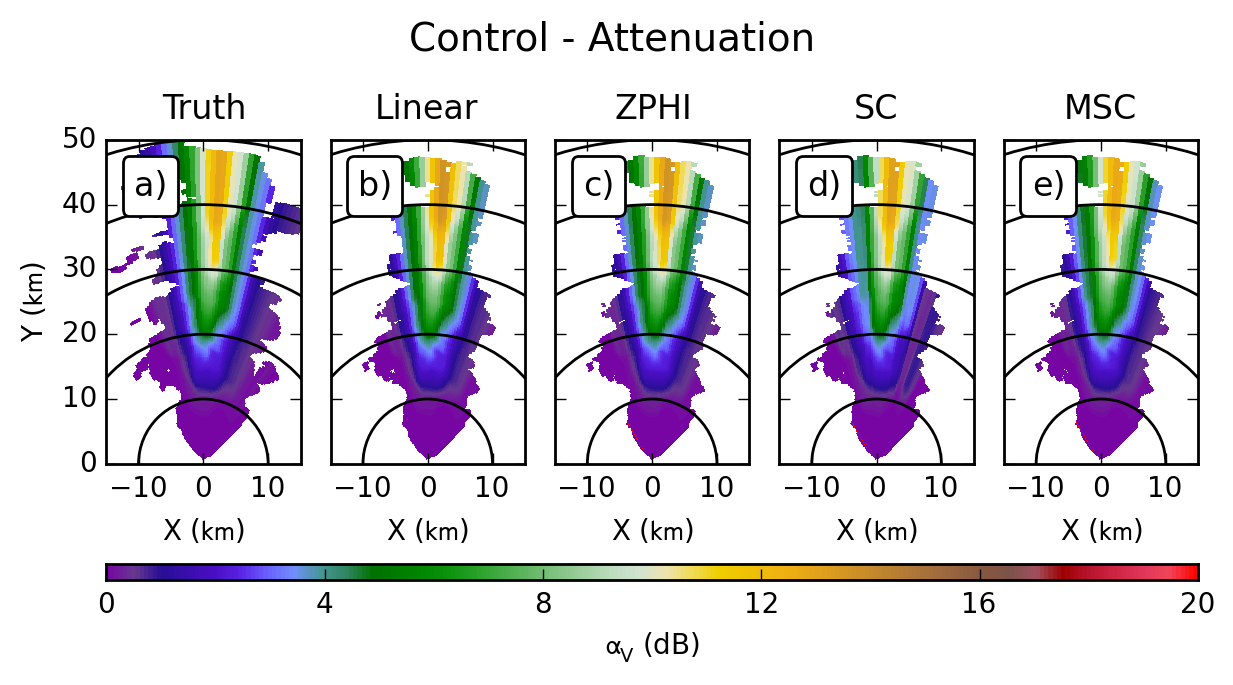
\includegraphics[scale=0.7]{figures/spatial/C_Control_Attenuation_V}
    \end{center}
\end{frame}

\begin{frame}
    \begin{center}
        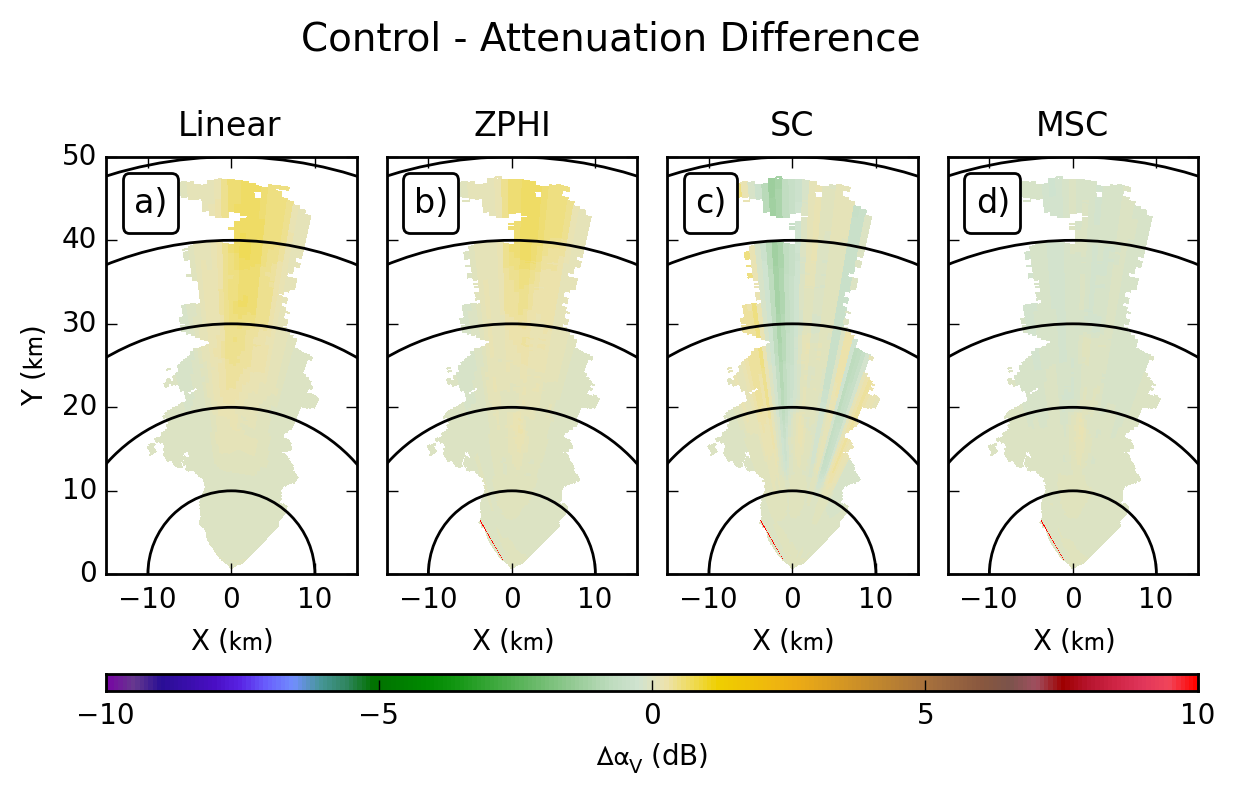
\includegraphics[scale=0.7]{figures/spatial/C_Control_Attenuation_Difference_V}
    \end{center}
\end{frame}

\begin{frame}
    \begin{center}
        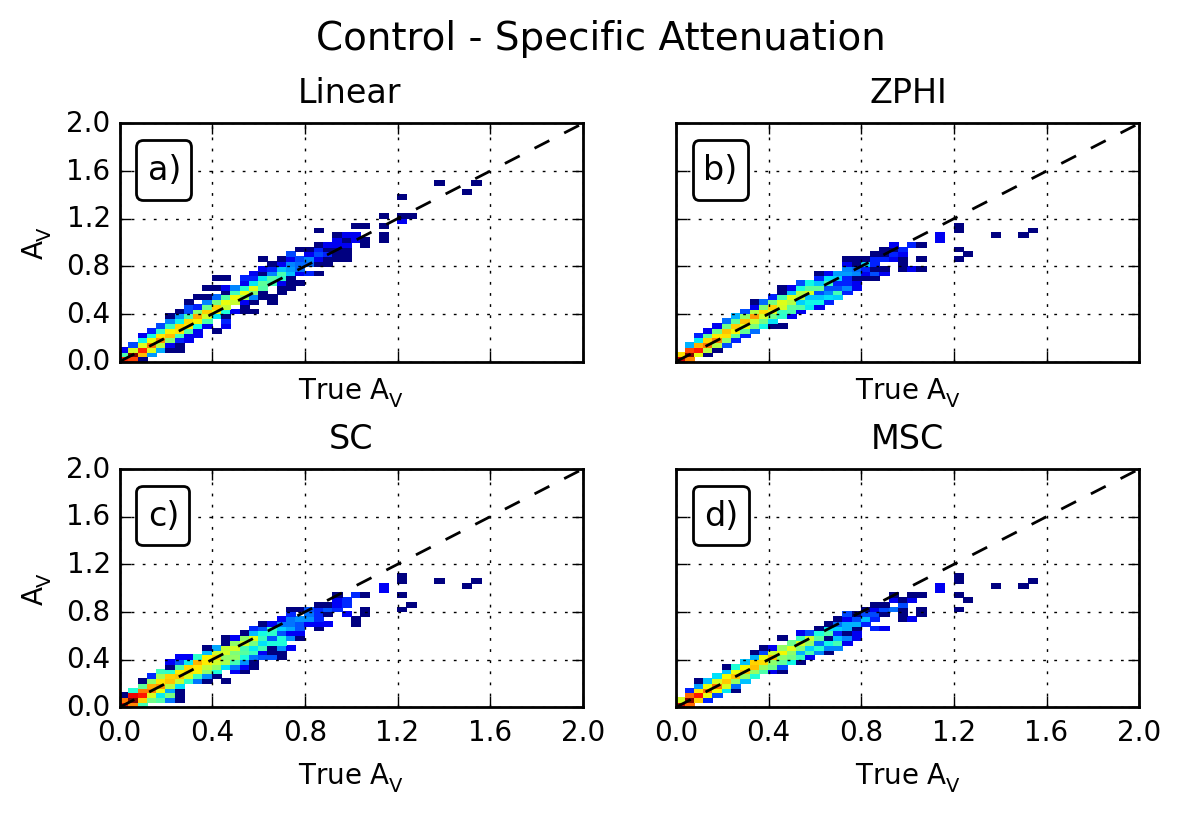
\includegraphics[scale=0.7]{figures/spatial/C_Control_Specific_Attenuation_V_scatter}
    \end{center}
\end{frame}

\begin{frame}
    \begin{center}
        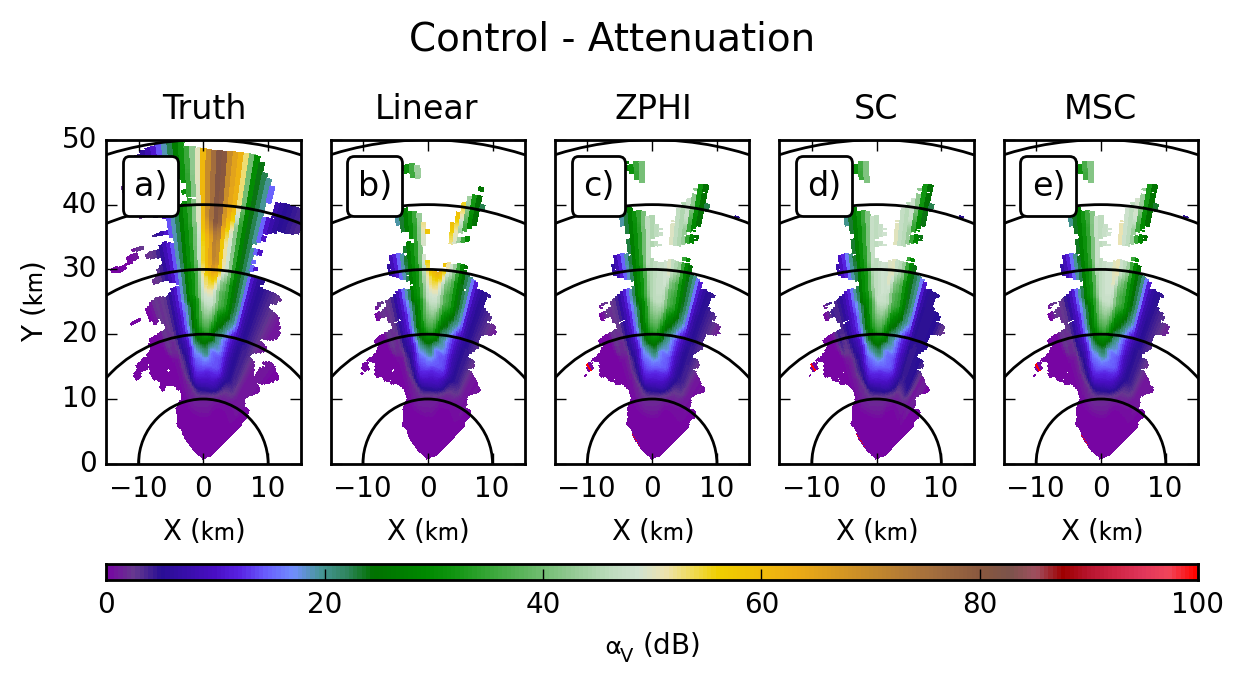
\includegraphics[scale=0.7]{figures/spatial/X_Control_Attenuation_V}
    \end{center}
\end{frame}

\begin{frame}
    \begin{center}
        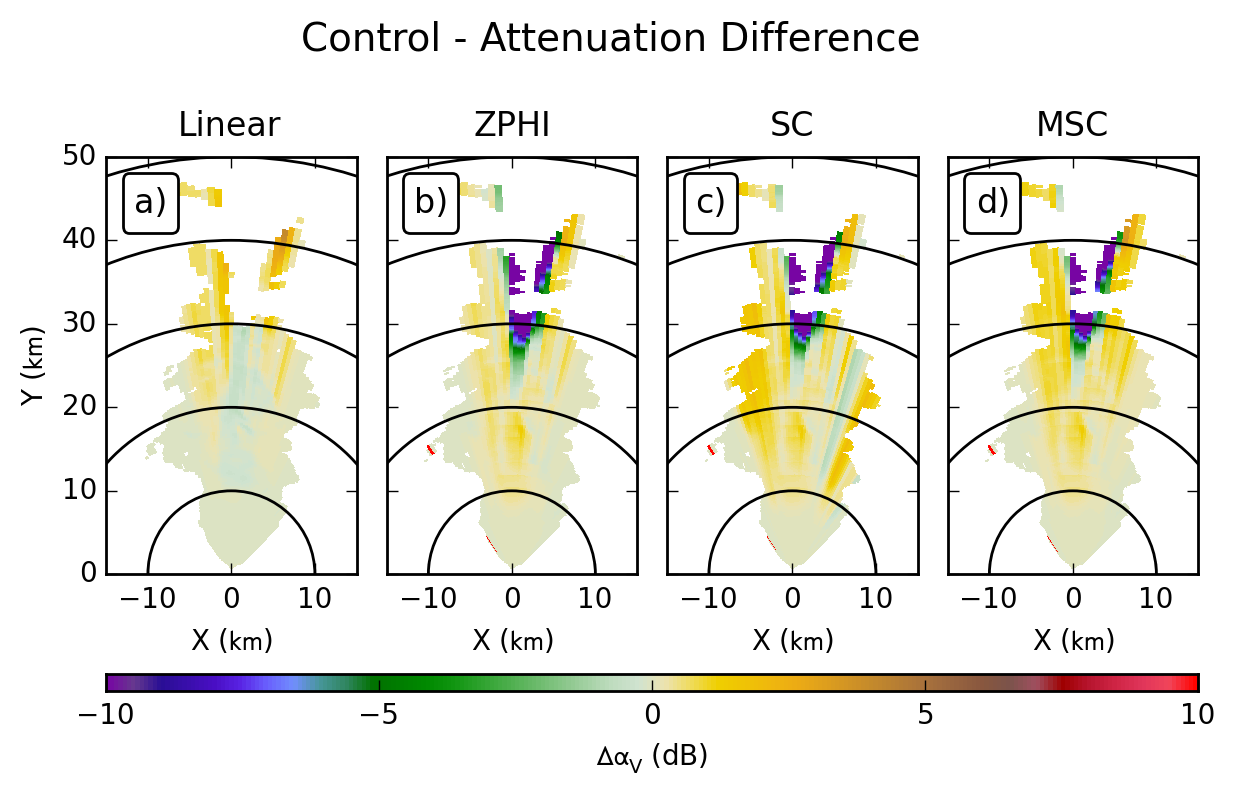
\includegraphics[scale=0.7]{figures/spatial/X_Control_Attenuation_Difference_V}
    \end{center}
\end{frame}

\begin{frame}
    \begin{center}
        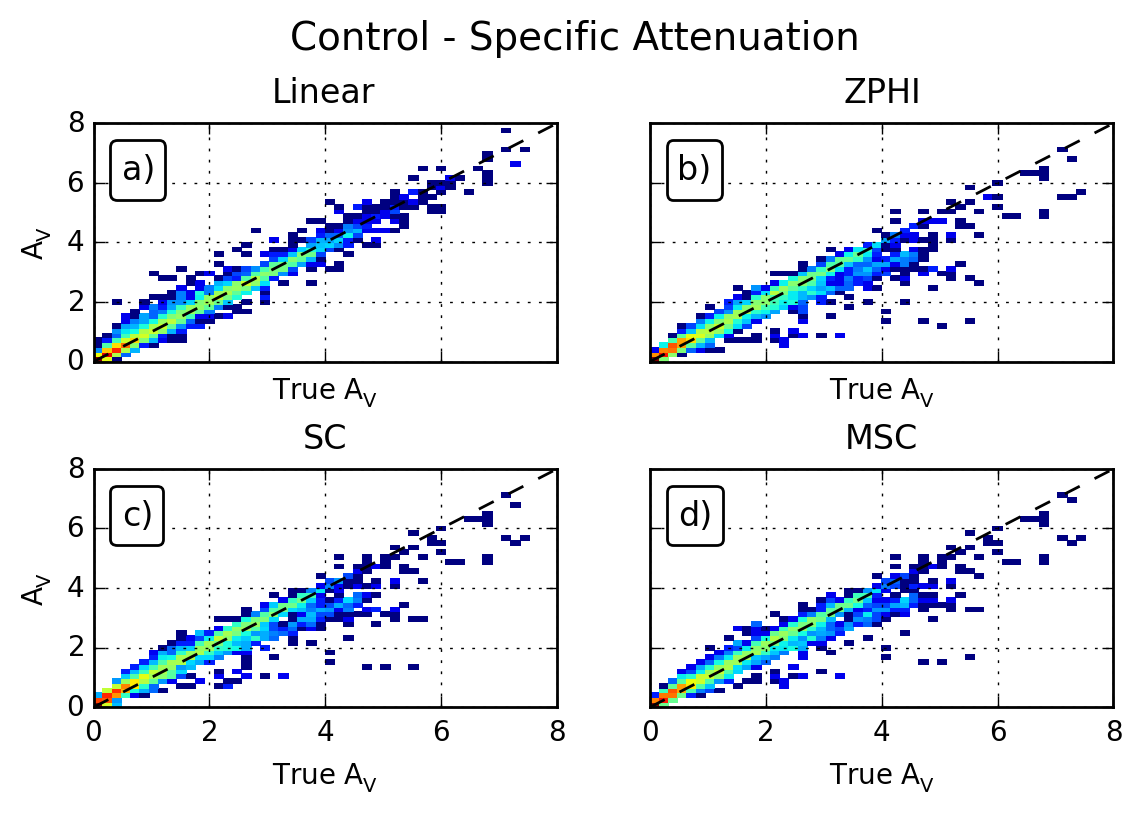
\includegraphics[scale=0.7]{figures/spatial/X_Control_Specific_Attenuation_V_scatter}
    \end{center}
\end{frame}

\begin{frame}
    \begin{center}
        \includegraphics<1>[scale=0.7]{figures/spatial/C_Sidelobe_Attenuation_V}
        \includegraphics<2>[scale=0.7]{figures/spatial/C_Control_Attenuation_V}
    \end{center}
\end{frame}

\begin{frame}
    \begin{center}
        \includegraphics<1>[scale=0.7]{figures/spatial/C_Sidelobe_Attenuation_Difference_V}
        \includegraphics<2>[scale=0.7]{figures/spatial/C_Control_Attenuation_Difference_V}
    \end{center}
\end{frame}

\begin{frame}
    \begin{center}
        \includegraphics<1>[scale=0.7]{figures/spatial/C_Sidelobe_Specific_Attenuation_V_scatter}
        \includegraphics<2>[scale=0.7]{figures/spatial/C_Control_Specific_Attenuation_V_scatter}
    \end{center}
\end{frame}

\begin{frame}
    \begin{center}
        \includegraphics<1>[scale=0.7]{figures/spatial/X_Sidelobe_Attenuation_V}
        \includegraphics<2>[scale=0.7]{figures/spatial/X_Control_Attenuation_V}
    \end{center}
\end{frame}

\begin{frame}
    \begin{center}
        \includegraphics<1>[scale=0.7]{figures/spatial/X_Sidelobe_Attenuation_Difference_V}
        \includegraphics<2>[scale=0.7]{figures/spatial/X_Control_Attenuation_Difference_V}
    \end{center}
\end{frame}

\begin{frame}
    \begin{center}
        \includegraphics<1>[scale=0.7]{figures/spatial/X_Sidelobe_Specific_Attenuation_V_scatter}
        \includegraphics<2>[scale=0.7]{figures/spatial/X_Control_Specific_Attenuation_V_scatter}
    \end{center}
\end{frame}

\begin{frame}
    \begin{center}
        \includegraphics<1>[scale=0.7]{figures/spatial/C_Beamwidth_Attenuation_V}
        \includegraphics<2>[scale=0.7]{figures/spatial/C_Control_Attenuation_V}
    \end{center}
\end{frame}

\begin{frame}
    \begin{center}
        \includegraphics<1>[scale=0.7]{figures/spatial/C_Beamwidth_Attenuation_Difference_V}
        \includegraphics<2>[scale=0.7]{figures/spatial/C_Control_Attenuation_Difference_V}
    \end{center}
\end{frame}

\begin{frame}
    \begin{center}
        \includegraphics<1>[scale=0.7]{figures/spatial/C_Beamwidth_Specific_Attenuation_V_scatter}
        \includegraphics<2>[scale=0.7]{figures/spatial/C_Control_Specific_Attenuation_V_scatter}
    \end{center}
\end{frame}

\begin{frame}
    \begin{center}
        \includegraphics<1>[scale=0.7]{figures/spatial/X_Beamwidth_Attenuation_V}
        \includegraphics<2>[scale=0.7]{figures/spatial/X_Control_Attenuation_V}
    \end{center}
\end{frame}

\begin{frame}
    \begin{center}
        \includegraphics<1>[scale=0.7]{figures/spatial/X_Beamwidth_Attenuation_Difference_V}
        \includegraphics<2>[scale=0.7]{figures/spatial/X_Control_Attenuation_Difference_V}
    \end{center}
\end{frame}

\begin{frame}
    \begin{center}
        \includegraphics<1>[scale=0.7]{figures/spatial/X_Beamwidth_Specific_Attenuation_V_scatter}
        \includegraphics<2>[scale=0.7]{figures/spatial/X_Control_Specific_Attenuation_V_scatter}
    \end{center}
\end{frame}

\begin{frame}
    \begin{center}
        \includegraphics<1>[scale=0.7]{figures/spatial/C_RadialWidth_Attenuation_V}
        \includegraphics<2>[scale=0.7]{figures/spatial/C_Control_Attenuation_V}
    \end{center}
\end{frame}

\begin{frame}
    \begin{center}
        \includegraphics<1>[scale=0.7]{figures/spatial/C_RadialWidth_Attenuation_Difference_V}
        \includegraphics<2>[scale=0.7]{figures/spatial/C_Control_Attenuation_Difference_V}
    \end{center}
\end{frame}

\begin{frame}
    \begin{center}
        \includegraphics<1>[scale=0.7]{figures/spatial/C_RadialWidth_Specific_Attenuation_V_scatter}
        \includegraphics<2>[scale=0.7]{figures/spatial/C_Control_Specific_Attenuation_V_scatter}
    \end{center}
\end{frame}

\begin{frame}
    \begin{center}
        \includegraphics<1>[scale=0.7]{figures/spatial/X_RadialWidth_Attenuation_V}
        \includegraphics<2>[scale=0.7]{figures/spatial/X_Control_Attenuation_V}
    \end{center}
\end{frame}

\begin{frame}
    \begin{center}
        \includegraphics<1>[scale=0.7]{figures/spatial/X_RadialWidth_Attenuation_Difference_V}
        \includegraphics<2>[scale=0.7]{figures/spatial/X_Control_Attenuation_Difference_V}
    \end{center}
\end{frame}

\begin{frame}
    \begin{center}
        \includegraphics<1>[scale=0.7]{figures/spatial/X_RadialWidth_Specific_Attenuation_V_scatter}
        \includegraphics<2>[scale=0.7]{figures/spatial/X_Control_Specific_Attenuation_V_scatter}
    \end{center}
\end{frame}

\begin{frame}
    \begin{center}
        \includegraphics<1>[scale=0.7]{figures/spatial/C_RangeResolution_Attenuation_V}
        \includegraphics<2>[scale=0.7]{figures/spatial/C_Control_Attenuation_V}
    \end{center}
\end{frame}

\begin{frame}
    \begin{center}
        \includegraphics<1>[scale=0.7]{figures/spatial/C_RangeResolution_Attenuation_Difference_V}
        \includegraphics<2>[scale=0.7]{figures/spatial/C_Control_Attenuation_Difference_V}
    \end{center}
\end{frame}

\begin{frame}
    \begin{center}
        \includegraphics<1>[scale=0.7]{figures/spatial/C_RangeResolution_Specific_Attenuation_V_scatter}
        \includegraphics<2>[scale=0.7]{figures/spatial/C_Control_Specific_Attenuation_V_scatter}
    \end{center}
\end{frame}

\begin{frame}
    \begin{center}
        \includegraphics<1>[scale=0.7]{figures/spatial/X_RangeResolution_Attenuation_V}
        \includegraphics<2>[scale=0.7]{figures/spatial/X_Control_Attenuation_V}
    \end{center}
\end{frame}

\begin{frame}
    \begin{center}
        \includegraphics<1>[scale=0.7]{figures/spatial/X_RangeResolution_Attenuation_Difference_V}
        \includegraphics<2>[scale=0.7]{figures/spatial/X_Control_Attenuation_Difference_V}
    \end{center}
\end{frame}

\begin{frame}
    \begin{center}
        \includegraphics<1>[scale=0.7]{figures/spatial/X_RangeResolution_Specific_Attenuation_V_scatter}
        \includegraphics<2>[scale=0.7]{figures/spatial/X_Control_Specific_Attenuation_V_scatter}
    \end{center}
\end{frame}

\begin{frame}
    \begin{center}
        \includegraphics<1>[scale=0.7]{figures/spatial/C_Combined_Attenuation_V}
        \includegraphics<2>[scale=0.7]{figures/spatial/C_Control_Attenuation_V}
    \end{center}
\end{frame}

\begin{frame}
    \begin{center}
        \includegraphics<1>[scale=0.7]{figures/spatial/C_Combined_Attenuation_Difference_V}
        \includegraphics<2>[scale=0.7]{figures/spatial/C_Control_Attenuation_Difference_V}
    \end{center}
\end{frame}

\begin{frame}
    \begin{center}
        \includegraphics<1>[scale=0.7]{figures/spatial/C_Combined_Specific_Attenuation_V_scatter}
        \includegraphics<2>[scale=0.7]{figures/spatial/C_Control_Specific_Attenuation_V_scatter}
    \end{center}
\end{frame}

\begin{frame}
    \begin{center}
        \includegraphics<1>[scale=0.7]{figures/spatial/X_Combined_Attenuation_V}
        \includegraphics<2>[scale=0.7]{figures/spatial/X_Control_Attenuation_V}
    \end{center}
\end{frame}

\begin{frame}
    \begin{center}
        \includegraphics<1>[scale=0.7]{figures/spatial/X_Combined_Attenuation_Difference_V}
        \includegraphics<2>[scale=0.7]{figures/spatial/X_Control_Attenuation_Difference_V}
    \end{center}
\end{frame}

\begin{frame}
    \begin{center}
        \includegraphics<1>[scale=0.7]{figures/spatial/X_Combined_Specific_Attenuation_V_scatter}
        \includegraphics<2>[scale=0.7]{figures/spatial/X_Control_Specific_Attenuation_V_scatter}
    \end{center}
\end{frame}

\begin{frame}
    \frametitle{Summary: MSE at C-band for Horizontal Polarization (\si{dB\squared\per \kilo\meter\squared})}
    \begin{center}
        \begin{tabular}{| c | c | c | c | c |}
            \hline
            Experiment & Linear & ZPHI & SC & MSC \\
            \hline
            \hline
            Control & 0.0030 & 0.0036 & 0.0035 & 0.0026 \\
            Beamwidth & 0.0029 & 0.0035 & 0.0032 & 0.0022 \\
            Radial Width & 0.0030 & 0.0036 & 0.0031 & 0.0022 \\
            Range Resolution & 0.0063 & 0.0038 & 0.0035 & 0.0027 \\
            Sidelobe & 0.0030 & 0.0036 & 0.0035 & 0.0025 \\
            Combined & 0.0564 & 0.0823 & 0.0043 & 0.0028 \\
            \hline
        \end{tabular}
    \end{center}
\end{frame}

\begin{frame}
    \frametitle{Summary: $r^2$ at C-band for Horizontal Polarization}
    \begin{center}
        \begin{tabular}{| c | c | c | c | c |}
            \hline
            Experiment & Linear & ZPHI & SC & MSC \\
            \hline
            \hline
            Control & 0.9789 & 0.9629 & 0.9573 & 0.9705 \\
            Beamwidth & 0.9808 & 0.9631 & 0.9582 & 0.9712 \\
            Radial Width & 0.9806 & 0.9622 & 0.9584 & 0.9716 \\
            Range Resolution & 0.9356 & 0.9590 & 0.9548 & 0.9690 \\
            Sidelobe & 0.9789 & 0.9630 & 0.9573 & 0.9706 \\
            Combined & 0.9661 & 0.7022 & 0.9294 & 0.9629 \\
            \hline
        \end{tabular}
    \end{center}
\end{frame}

\begin{frame}
    \frametitle{Summary: Bias at C-band for Vertical Polarization (\si{dB\per \kilo\meter})}
    \begin{center}
        \begin{tabular}{| c | c | c | c | c |}
            \hline
            Experiment & Linear & ZPHI & SC & MSC \\
            \hline
            \hline
            Control & 0.0101 & 0.0079 & -0.0031 & -0.0055 \\
            Beamwidth & 0.0115 & 0.0091 & -0.0037 & -0.0063 \\
            Radial Width & 0.0121 & 0.0099 & -0.0019 & -0.0007 \\
            Range Resolution & 0.0101 & 0.0078 & -0.0065 & -0.0114 \\
            Sidelobe & 0.0101 & 0.0079 & -0.0032 & -0.0055 \\
            Combined & 0.1445 & 0.1419 & 0.0079 & -0.0028 \\
            \hline
        \end{tabular}
    \end{center}
\end{frame}

\begin{frame}
    \frametitle{Summary: MSE at C-band for Vertical Polarization (\si{dB\squared\per \kilo\meter\squared})}
    \begin{center}
        \begin{tabular}{| c | c | c | c | c |}
            \hline
            Experiment & Linear & ZPHI & SC & MSC \\
            \hline
            \hline
            Control & 0.0011 & 0.0014 & 0.0021 & 0.0014 \\
            Beamwidth & 0.0011 & 0.0013 & 0.0020 & 0.0013 \\
            Radial Width & 0.0011 & 0.0013 & 0.0018 & 0.0012 \\
            Range Resolution & 0.0029 & 0.0014 & 0.0022 & 0.0016 \\
            Sidelobe & 0.0011 & 0.0014 & 0.0021 & 0.0014 \\
            Combined & 0.0339 & 0.0416 & 0.0019 & 0.0012 \\
            \hline
        \end{tabular}
    \end{center}
\end{frame}

\begin{frame}
    \frametitle{Summary: $r^2$ at C-band for Vertical Polarization}
    \begin{center}
        \begin{tabular}{| c | c | c | c | c |}
            \hline
            Experiment & Linear & ZPHI & SC & MSC \\
            \hline
            \hline
            Control & 0.9820 & 0.9665 & 0.9493 & 0.9686 \\
            Beamwidth & 0.9829 & 0.9668 & 0.9514 & 0.9694 \\
            Radial Width & 0.9832 & 0.9665 & 0.9527 & 0.9693 \\
            Range Resolution & 0.9368 & 0.9642 & 0.9467 & 0.9677 \\
            Sidelobe & 0.9820 & 0.9665 & 0.9493 & 0.9687 \\
            Combined & 0.9759 & 0.7687 & 0.9240 & 0.9644 \\
            \hline
        \end{tabular}
    \end{center}
\end{frame}

\begin{frame}
    \frametitle{Summary: MSE at C-band for Differential Polarization (\si{dB\squared\per \kilo\meter\squared})}
    \begin{center}
        \begin{tabular}{| c | c | c | c | c |}
            \hline
            Experiment & Linear & ZPHI & SC & MSC \\
            \hline
            \hline
            Control & 0.0020 & 0.0014 & 0.0007 & 0.0005 \\
            Beamwidth & 0.0019 & 0.0014 & 0.0007 & 0.0006 \\
            Radial Width & 0.0019 & 0.0014 & 0.0006 & 0.0004 \\
            Range Resolution & 0.0023 & 0.0015 & 0.0007 & 0.0005 \\
            Sidelobe & 0.0020 & 0.0014 & 0.0007 & 0.0005 \\
            Combined & 0.0079 & 0.0141 & 0.0009 & 0.0007 \\
            \hline
        \end{tabular}
    \end{center}
\end{frame}

\begin{frame}
    \frametitle{Summary: $r^2$ at C-band for Differential Polarization}
    \begin{center}
        \begin{tabular}{| c | c | c | c | c |}
            \hline
            Experiment & Linear & ZPHI & SC & MSC \\
            \hline
            \hline
            Control & 0.9380 & 0.8904 & 0.8911 & 0.9453 \\
            Beamwidth & 0.9456 & 0.8880 & 0.8975 & 0.9478 \\
            Radial Width & 0.9479 & 0.8851 & 0.8937 & 0.9461 \\
            Range Resolution & 0.8609 & 0.8741 & 0.8822 & 0.9445 \\
            Sidelobe & 0.9380 & 0.8903 & 0.8910 & 0.9530 \\
            Combined & 0.9179 & 0.2917 & 0.8761 & 0.9411 \\
            \hline
        \end{tabular}
    \end{center}
\end{frame}

\begin{frame}
    \frametitle{Summary: MSE at X-band for Horizontal Polarization (\si{dB\squared\per \kilo\meter\squared})}
    \begin{center}
        \begin{tabular}{| c | c | c | c | c |}
            \hline
            Experiment & Linear & ZPHI & SC & MSC \\
            \hline
            \hline
            Control & 0.0501 & 0.1266 & 0.1244 & 0.1105 \\
            Beamwidth & 0.0974 & 0.1231 & 0.1277 & 0.3123 \\
            Radial Width & 0.1477 & 0.1567 & 0.1521 & 0.2799 \\
            Range Resolution & 0.1286 & 0.1114 & 0.1136 & 0.0966 \\
            Sidelobe & 0.0501 & 0.1206 & 0.1187 & 0.0986 \\
            Combined & 0.3601 & 0.7653 & 0.1962 & 0.1902 \\
            \hline
        \end{tabular}
    \end{center}
\end{frame}

\begin{frame}
    \frametitle{Summary: $r^2$ at X-band for Horizontal Polarization}
    \begin{center}
        \begin{tabular}{| c | c | c | c | c |}
            \hline
            Experiment & Linear & ZPHI & SC & MSC \\
            \hline
            \hline
            Control & 0.9789 & 0.9453 & 0.9468 & 0.9526 \\
            Beamwidth & 0.9596 & 0.9415 & 0.9413 & 0.8805 \\
            Radial Width & 0.9379 & 0.9216 & 0.9264 & 0.8775 \\
            Range Resolution & 0.9425 & 0.9504 & 0.9500 & 0.9560 \\
            Sidelobe & 0.9789 & 0.9482 & 0.9495 & 0.9562 \\
            Combined & 0.9675 & 0.8163 & 0.9300 & 0.9322 \\
            \hline
        \end{tabular}
    \end{center}
\end{frame}

\begin{frame}
    \frametitle{Summary: Bias at X-band for Vertical Polarization (\si{dB\per \kilo\meter})}
    \begin{center}
        \begin{tabular}{| c | c | c | c | c |}
            \hline
            Experiment & Linear & ZPHI & SC & MSC \\
            \hline
            \hline
            Control & 0.0254 & -0.0131 & 0.0260 & 0.0152 \\
            Beamwidth & 0.0730 & 0.0303 & 0.0574 & 0.0909 \\
            Radial Width & 0.0969 & 0.0514 & 0.0750 & 0.1016 \\
            Range Resolution & 0.0237 & -0.0190 & 0.0114 & 0.0037 \\
            Sidelobe & 0.0254 & -0.0162 & 0.0230 & 0.0167 \\
            Combined & 0.4151 & 0.3743 & 0.0455 & 0.0374 \\
            \hline
        \end{tabular}
    \end{center}
\end{frame}

\begin{frame}
    \frametitle{Summary: MSE at X-band for Vertical Polarization (\si{dB\squared\per \kilo\meter\squared})}
    \begin{center}
        \begin{tabular}{| c | c | c | c | c |}
            \hline
            Experiment & Linear & ZPHI & SC & MSC \\
            \hline
            \hline
            Control & 0.0335 & 0.0789 & 0.0774 & 0.0670 \\
            Beamwidth & 0.0762 & 0.0921 & 0.0974 & 0.1060 \\
            Radial Width & 0.1074 & 0.1131 & 0.1187 & 0.1394 \\
            Range Resolution & 0.0900 & 0.0859 & 0.0869 & 0.0751 \\
            Sidelobe & 0.0336 & 0.0898 & 0.0884 & 0.0760 \\
            Combined & 0.2852 & 0.8375 & 0.1177 & 0.1245 \\
            \hline
        \end{tabular}
    \end{center}
\end{frame}

\begin{frame}
    \frametitle{Summary: $r^2$ at X-band for Vertical Polarization}
    \begin{center}
        \begin{tabular}{| c | c | c | c | c |}
            \hline
            Experiment & Linear & ZPHI & SC & MSC \\
            \hline
            \hline
            Control & 0.9793 & 0.9518 & 0.9529 & 0.9580 \\
            Beamwidth & 0.9537 & 0.9389 & 0.9371 & 0.9334 \\
            Radial Width & 0.9340 & 0.9215 & 0.9199 & 0.9095 \\
            Range Resolution & 0.9424 & 0.9455 & 0.9448 & 0.9513 \\
            Sidelobe & 0.9793 & 0.9444 & 0.9452 & 0.9516 \\
            Combined & 0.9677 & 0.7451 & 0.9376 & 0.9343 \\
            \hline
        \end{tabular}
    \end{center}
\end{frame}

\begin{frame}
    \frametitle{Summary: MSE at X-band for Differential Polarization (\si{dB\squared\per \kilo\meter\squared})}
    \begin{center}
        \begin{tabular}{| c | c | c | c | c |}
            \hline
            Experiment & Linear & ZPHI & SC & MSC \\
            \hline
            \hline
            Control & 0.0031 & 0.0087 & 0.0085 & 0.0364 \\
            Beamwidth & 0.0030 & 0.0135 & 0.0115 & 0.1543 \\
            Radial Width & 0.0030 & 0.0169 & 0.0106 & 0.0694 \\
            Range Resolution & 0.0056 & 0.0092 & 0.0105 & 0.0099 \\
            Sidelobe & 0.0031 & 0.0103 & 0.0100 & 0.0102 \\
            Combined & 0.0076 & 0.2471 & 0.0170 & 0.0195 \\
            \hline
        \end{tabular}
    \end{center}
\end{frame}

\begin{frame}
    \frametitle{Summary: $r^2$ at X-band for Differential Polarization}
    \begin{center}
        \begin{tabular}{| c | c | c | c | c |}
            \hline
            Experiment & Linear & ZPHI & SC & MSC \\
            \hline
            \hline
            Control & 0.9752 & 0.8600 & 0.8637 & 0.7057 \\
            Beamwidth & 0.9776 & 0.7606 & 0.7927 & 0.3618 \\
            Radial Width & 0.9782 & 0.6911 & 0.7978 & 0.4196 \\
            Range Resolution & 0.9295 & 0.8442 & 0.8192 & 0.8321 \\
            Sidelobe & 0.9752 & 0.8333 & 0.8412 & 0.8509 \\
            Combined & 0.9709 & 0.3742 & 0.8062 & 0.7740 \\
            \hline
        \end{tabular}
    \end{center}
\end{frame}

\setcounter{framenumber}{\value{finalframe}}
\end{document}